%% LyX 2.0.6 created this file.  For more info, see http://www.lyx.org/.
%% Do not edit unless you really know what you are doing.
\documentclass[11pt,twoside,english,italian]{report}
\renewcommand{\ttdefault}{mathpazo}
\usepackage[T1]{fontenc}
\usepackage[utf8]{inputenc}
\usepackage[a4paper]{geometry}
\geometry{verbose}
\setcounter{secnumdepth}{3}
\setcounter{tocdepth}{3}
\usepackage{fancybox}
\usepackage{calc}
\usepackage{textcomp}
\usepackage{amsmath}
\usepackage{amssymb}
\PassOptionsToPackage{normalem}{ulem}
\usepackage{ulem}

\makeatletter

%%%%%%%%%%%%%%%%%%%%%%%%%%%%%% LyX specific LaTeX commands.
\newcommand{\lyxmathsym}[1]{\ifmmode\begingroup\def\b@ld{bold}
  \text{\ifx\math@version\b@ld\bfseries\fi#1}\endgroup\else#1\fi}

%% Because html converters don't know tabularnewline
\providecommand{\tabularnewline}{\\}

%%%%%%%%%%%%%%%%%%%%%%%%%%%%%% User specified LaTeX commands.

\newlength\tindent
\setlength{\tindent}{\parindent}
\setlength{\parindent}{0pt}
\renewcommand{\indent}{\hspace*{\tindent}}

\providecommand{\coursename}{Logica e Algebra 2}
\providecommand{\documentsubtitle}{Appunti}
\providecommand{\annoacc}{2013-2014}
\providecommand{\principaladviser}{Prof. Alessandra Cherubini}
\providecommand{\firstauthor}{Edoardo Pasi}
\providecommand{\firstauthorid}{805753}
\providecommand{\secondauthor}{Davide Tateo}
\providecommand{\secondauthorid}{799311}
\title{Logica e Algebra 2}
\author{\firstauthor, \secondauthor}

 
\usepackage{tikz}
\usepackage{stmaryrd}

\usepackage{color}   %May be necessary if you want to color links
\usepackage{hyperref}
\hypersetup{
    colorlinks=true, %set true if you want colored links
    linktoc=all,     %set to all if you want both sections and subsections linked
    linkcolor=black,  %choose some color if you want links to stand out
}

\usepackage{booktabs}
\usepackage{listings}
\lstset{columns=fullflexible}

\usepackage{wasysym}

\usepackage{amsthm}
\newtheoremstyle{note} % name
{\topsep} 	% Space above
{\topsep} 	% Space below
{\small}		% Body font
{}		% Indent amount
{\small\bfseries}% Theorem head font
{:}		% Punctuation after theorem head
{.5em}	% Space after theorem head
{}		% Theorem head spec (can be left empty, meaning ‘normal’)

\usepackage{fancyhdr}%% Cambia il carattere delle didascalie delle figure %%
\usepackage[font=small,format=plain,labelfont=bf,up,textfont=it,up]{caption}

\usepackage{comment}

%per le tabelle lunghe e particolari
\usepackage{lscape}
%per includere il comando che genera la pagina del titolo...
\usepackage{settings/frontesp}

\makeatother

\usepackage{babel}
\begin{document}
\titlep

\tableofcontents{}

\selectlanguage{english}%
\global\long\def\veraw#1#2#3{#1\models_{#2}#3}


\global\long\def\vera#1#2{#1\models#2}


\global\long\def\nonvera#1#2{#1\nvDash#2}


\global\long\def\nonveraw#1#2#3{#1\nvDash_{#2}#3}


\global\long\def\nonSem#1#2{#1\nvdash#2}


\global\long\def\nonTeor#1#2{\nvdash_{#1}#2}


\global\long\def\nonSemW#1#2#3{#1\nvdash_{#2}#3}


\global\long\def\verita#1#2{#1\in V(#2)}


\global\long\def\entail#1#2{#1\models#2}


\global\long\def\semantica#1#2#3{#1\vdash_{#2}#3}


\global\long\def\teolm#1#2{\vdash_{#1}#2}


\global\long\def\semGen#1#2{#1\vdash#2}


\global\long\def\boxx#1{\square#1}


\global\long\def\diam#1{\diamond#1}


\global\long\def\dia{\diamond a}


\global\long\def\boa{\boxx a}


\global\long\def\noa{\neg a}


\global\long\def\forhten#1#2#3{\forall#1#2\implies#3}


\global\long\def\implica#1#2{#1\implies#2}


\global\long\def\teorema#1{\vdash_{\Lambda}#1}


\global\long\def\teorGamma#1{\Gamma\vdash_{\Lambda}#1}


\global\long\def\teoa{\teorGamma a}


\global\long\def\teoremaDi#1{\vdash_{#1}}


\global\long\def\consist{\mbox{\ensuremath{\Lambda}}-consistente}


\global\long\def\consMax{\Lambda-consistente\: massimale}


\global\long\def\veraCanAlfa#1{\vera{M^{\Lambda}}{_{\alpha}}#1}


\global\long\def\veraCA{\vera{M^{\Lambda}}{_{\alpha}}a}


\global\long\def\veraCan#1#2{\vera{M^{\Lambda}}{_{#1}}#2}


\global\long\def\nonveraCan#1#2{\nonveraw{M^{\Lambda}}{#1}{#2}}


\global\long\def\consMaxLog#1{#1-consistente\ massimale}


\global\long\def\relazCAB#1#2{\{a\ |\ \boa\in#1\}\subseteq#2}


\global\long\def\relazCAD#1#2{\{\diamond b\ |\ b\in#2\}\subseteq#1}


\global\long\def\andoria#1{a_{1}\wedge...\wedge a#1}


\global\long\def\andbox#1{\boa_{1}\wedge\dots\wedge\boxx a#1}


\global\long\def\neci#1#2{[#1]#2}


\global\long\def\posi#1#2{<#1>#2}


\global\long\def\necf#1{[F]#1}


\global\long\def\posf#1{<F>#1}


\global\long\def\necp#1{[P]#1}


\global\long\def\posp#1{<P>#1}


\global\long\def\verins#1{\Vert#1\Vert^{\mu}}


\global\long\def\verinsx#1#2{\Vert#1\Vert^{\mu^{#2}}}


\global\long\def\cardinal#1{\Vert#1\Vert}


\global\long\def\alue{AL\mbox{\ensuremath{\mathcal{UE}}}}


\global\long\def\alc{AL\mbox{\ensuremath{\mathcal{\mathcal{C}}}}}
	

\global\long\def\globally#1{\mathcal{G}#1}


\global\long\def\eventually#1{\mathcal{F}#1}


\global\long\def\next#1{\mathcal{X}#1}


\global\long\def\until#1#2{#1\mathcal{U}#2}


\global\long\def\release#1#2{#1\mathcal{R}#2}
\selectlanguage{italian}%




\chapter{Introduzione}

\label{cap:introduction}


\section{Intro}

Se voi signorine finirete questo corso, e se sopravviverete sarete
dispensatori di fbf e pregherete per modellizzare sistemi assurdi
in modo ancora più assurdo, ma fino a quel giorno non siete altro
che buoni annulla convinti che tutti i cretesi sono stupidi e forse
mentono.

Lasciate il formaggio fuori dall'aula.


\global\long\def\veraw#1#2#3{#1\models_{#2}#3}
 

\global\long\def\vera#1#2{#1\models#2}


\global\long\def\verita#1#2{#1\in V(#2)}
 

\global\long\def\entail#1#2{#1\models#2}
 

\global\long\def\semantica#1#2#3{#1\vdash_{#2}#3}


\global\long\def\semGen#1#2{#1\vdash#2}


\global\long\def\boxx#1{\square#1}


\global\long\def\diam#1{\diamond#1}


\global\long\def\dia{\diamond a}


\global\long\def\boa{\boxx a}


\global\long\def\forhten#1#2#3{\forall#1#2\Rightarrow#3}


\global\long\def\implica#1#2{#1\Rightarrow#2}



\chapter{Introduction}

$a$ è vera nel mondo $\alpha$, e scriviamo $\mu\models_{\alpha}a$

se
\begin{itemize}
\item $a$ è una lettera enunciativa allora deve valere $\verita a{\alpha}$ 
\item $a$ è del tipo: $a\lor b$ .... allora.... $\mu\models_{\alpha}a$
oppure $\mu\models_{\alpha}b$
\end{itemize}

\section{Formule di Logica modale e significato}

\begin{tabular}{|c|c|c|}
\hline 
$\diam{}{a\Rightarrow}\boxx a$  & funzione parziale & $\forhten{\alpha}{:\,\alpha R\beta,\:\beta R\gamma}{\beta}=\gamma$\tabularnewline
\hline 
\end{tabular}

Funzione parziale, dimostrazione

.

Ip) funzione parziale 

Ts) $\diam{}{a\Rightarrow}\boxx a$

.

$\diam{}a$ falsa allora dato che l'antecedente è falso di ha $\implica{\diam{}a}{\boxx a}$

$\diam{}a$ vera allora $\exists\beta$:$\alpha R\beta$ e$\in V(\beta)$,
ma dato che la funzione è parziale questo $\beta$ è unico !

da cui $\vera{\mu}{\implica{\diamond a}{\boxx a}}$

.

.

Ip) $\diam{}{a\Rightarrow}\boxx a$

Ts) funzione parziale

.

.

Per assurdo: suppongo non che la funzione non sia parziale. Se è così
$\exists\alpha:$ $\alpha R\beta,$ $\alpha R\gamma$, considero un
modello in cui V(A) = \{$\beta$ \} , $\boxx A$ non vale in $\alpha$
dato che A è falsa in $\gamma$, il che contraddice l'ipotesi (BAM!)\\\\

\begin{tabular}{|c|c|c|}
\hline 
$\diam{}{a\iff}\boxx a$  & funzione totale & $\forall\alpha\exists\,!\,\beta:\:\alpha R\beta$ \tabularnewline
\hline 
\end{tabular}\\\\

non ci sono ``conti'' da fare, R è seriale sse R è seriale $\boxx a\implies\diam a$
, e se R è una funzione parziale $\implica{\diam a}{\boxx a}$

quindi dato che l'implica prevede un and di implica da una parte e
dall'altra per definizione abbiamo la tesi

.

.

\begin{tabular}{|c|c|c|}
\hline 
$\diam{}{a\Rightarrow}\boxx{\diam a}$  & relazione euclidea & $\forhten{\alpha,\beta,\gamma}{:\:(\alpha R\beta,\:\alpha R\gamma)}{\beta}R\gamma$
da cui anche: $\beta$R$\beta$, $\gamma R\gamma$, $\gamma$R$\beta$\tabularnewline
\hline 
\end{tabular} \\\\

Ip) relazione euclidea

Ts) $\diam{}{a\Rightarrow}\boxx{\diam a}$ 

Suppongo sia vero l'antecedente (se falso ho finito), quindi vale:
$\dia$ da cui: $\vera{\mu}{\dia}$

dato che $\dia$ si ha che esiste almeno un $\beta$ tale che in beta
vale a 

solo un beta: autoanello perché euclidea e quindi $\boxx{\dia}$

diversi beta: ognuno dei vari $\beta'$, $\beta''$ , ecc. sono in
relazione con $\beta$, dato che la relazione è euclidea, pertanto
dato che in $\beta$ vale $a$, in ognuno di loro vale $\dia$ \\

Ip)$\diam{}{a\Rightarrow}\boxx{\diam a}$ 

Ts) relazione euclidea

Per assurdo, suppondo valga ip) ma non la tesi

Considero un Frame in cui: $\alpha R\beta,$ $\alpha R\gamma,$ $\beta R\gamma$
ma NON $\beta R\gamma$ cioè si ha un frammento in cui non vale l'euclidea.
Poniamo che il modello sia tale che $V(A)$$=\{\gamma\}$

In queste ipotesi vale $\dia$ dato che in $\gamma$ vale $a$. In
$\beta$ non vale $a$ e neppure $\dia$ perché non ha ``uscite'',
da cui in $a$ non vale $\boxx{\dia}$ contraddicendo così l'ipotesi
(BAM!) \\\\


\section{Semantica}

$\semGen ab$ cioè a è conseguenza semantica di b, se in ogni Frame,
Modello e Mondo in cui $\vera{\mu}b$ si ha anche $\vera{\mu}a$\\

$\dia\equiv\sim\boxx{\sim a}$

Vale da sinistra a destra,

Infatti:

se $\veraw{\mu}{\alpha}{\dia}$ allora 

$\exists\beta:$$\alpha R\beta$ e $\veraw{\mu}{\beta}a$ da cui:

$\mu\nvDash_{\beta}\sim a$

per questo in $\alpha$ non vale $\boxx{\sim a}$ (perché non vale
$\sim a$ in $\beta$)

allora in $\alpha$ vale $\sim\boxx{\sim a}$ cioè $\veraw{\mu}{\alpha}{\sim\boxx{\sim a}}$
cioè la tesi. \\

Vale anche da destra a sinistra, dimostrazione simile.



\chapter{Semantica}


\section{Simboli secessari}

$\semGen ab$ cioè a è conseguenza semantica di b, se in ogni Frame,
Modello e Mondo in cui $\vera\mu b$ si ha anche $\vera\mu a$\\


$\dia\equiv\neg\boxx{\neg a}$

Vale da sinistra a destra,

Infatti:

se $\veraw\mu\alpha\dia$ allora

$\exists\beta:$$\alpha R\beta$ e $\veraw\mu\beta a$ da cui:

$\mu\nvDash_{\beta}\neg a$

per questo in $\alpha$ non vale $\boxx{\neg a}$ (perché non vale
$\neg a$ in $\beta$)

allora in $\alpha$ vale $\neg\boxx{\neg a}$ cioè $\veraw\mu\alpha{\neg\boxx{\neg a}}$
cioè la tesi. \\


Vale anche da destra a sinistra, dimostrazione simile. \\



\section{Logiche}

Una logica $\Lambda$ su L è un insieme di fbf su L che: 
\begin{itemize}
\item contiene tutte le tautologie 
\item è chiusa rispetto al Modus Ponens 
\end{itemize}
Ad esempio; $PL(\phi)$ cioè i teoremi della logica proposizionale

Altro esempio $\Lambda_{C}=\{a\,|\,\vera F{a\: per}\ ogni\ F\in C\}$

infatti: 
\begin{itemize}
\item contiene tutte le tautologie perché sono vere mondo per mondo dappertutto 
\item MP : suppongo che in un mondo $\alpha$ accada che: $\nonveraw{\mu}{\alpha}b$
, $\veraw{\mu}{\alpha}a$ . Se vale anche $\veraw{\mu}{\alpha}{\implica ab}$
... l'antecedente è vero, quindi dato che l'implicazione è vera, deve
essere vero anche il conseguente da cui non può che essere $\veraw{\mu}{\alpha}b$ 
\end{itemize}
Una logica si dice \textbf{uniforme }se è chiusa rispetto a sostituzioni
uniformi cioè se sostituendo a una lettere uguali formule uguali in
una tautologia, ottengo una tautologia.

Es. $\Lambda_{C}=\{a\,|\,\vera F{a\: per}\ ogni\ F\in C\}$ NON è
uniforme infatti se considero $V(A)=S$, dove S sono tutti gli stati
possibili (mondi), vale anche $\veraw{\mu}{\alpha}A$, e cioè A è
una tautologia, se al posto di A sostituisco $B\wedge\neg B$ (falsa
in ogni modello e mondo) non ottengo una tautologia.\\
 \\


\textbf{\emph{\large{{{{Teorema}}}}}}{\large \par}

Sono equivalenti: 
\begin{enumerate}
\item $\Lambda$ è normale 
\item per ogni intero n $\geq0$,


$\teorema{a1\wedge a2\wedge...\wedge an}\implies a$ implica $\teorema{\boa1\wedge\boa2\wedge...\wedge\boa n}\implies\boa$

\item valgono:

\begin{enumerate}
\item $\teorema{\boxx T}$ 
\item $\teorema{\boa\wedge\boxx b}\implies\boxx{(a\wedge b)}$ 
\item $\teorema{\implica ab}$ implica $\teorema{\boa\implies\boxx b}$ 
\end{enumerate}
\end{enumerate}
Dimostrazione

$1\implies$2

per induzione.

se n = 0 allora $\teorema a$ allora $\teorema{\boa}$ per la regola
RN che vale in $\Lambda$ per ipotesi

se n > 0 (passo induttivo) suppongo valga l'antecedente, altrimenti
2 vale senz'altro;

Ricordiamo che $a1\wedge a2\wedge...\wedge an\implies a\equiv a1\wedge a2\wedge...a_{n-1}\implies(an\implies a)$ 


\begin{savequote}[60mm]
Senza dubbio questo era un piano eccellente, semplice e davvero ben congegnato. \\
C'era solo una difficoltà: che Alice non aveva la più piccola idea di come realizzarlo.
\qauthor{Lewis Carroll} \end{savequote}


\chapter{Verso la decidibilità - Logica determinata}


\section{Insieme $\Lambda$ consistente e sue proprietà}

Sia $\Lambda$ una logica (cioè ha tutte le tautologie ed è chiusa
rispetto al Modus Ponens)	

$\Gamma$ si dice $\Lambda$-consistente se: $\nonSinW{\Gamma}{\Lambda}{\bot}$,
dove $\bot=A\wedge\neg A$

$\Delta$ si dice $\Lambda$-consistente massimale se per ogni fbf
$a$ $a\in\Delta$ oppure $\neg a\in\Delta$ $ $\\


\textbf{Proprietà:} $ $ 
\begin{enumerate}
\item Se $\teoa$ e $\Gamma\subseteq\Delta$ allora $\Delta\teorema a$.
Ovvero se alcune premesse non mi servono posso comunque metterle per
dedurre una formula 
\item Se $\teorGamma a$ e $\Lambda\subseteq\Lambda'$ allora $\Gamma\vdash_{\Lambda'}a$.
Ovvero quello che posso dedurre in una logica più scarna (es. PL)
lo posso dedurre anche in una più ricca che la contiene (es. Modale) 
\item se $a\in\Gamma$ allora $\teoa$ . \\
 Infatti $\teorema{a\implies a}$ è un teorema dato che $a\implies a$
è una tautologia 
\item $\{a|\teoa\}$ è la minima logica che contiene $\Gamma\cup\Lambda$.
Infatti posso dedurre tutte le tautologie da $\Gamma$, anche se non
userò nessuna formula di $\Gamma$ ma solo quelle che già sono nella
logica $\Lambda$ $ $ 
\item Se $\teoa$ e $\{a\}$$\teorema b$ allora $\teorGamma b$ \\
 Infatti: per dedurre $a$ uso regole di inferenza, formule di $\Gamma$,
assiomi di $\Lambda$. Per arrivare in $b$ uso assiomi di $\Lambda$
e regole di inferenza, quindi posso arrivare da $\Gamma$ direttamente
in $b$ usando formule di $\Gamma$, regole di inf. e assiomi di $\Lambda$ 
\item Se $\teoa$ e $\teorGamma{\implica ab}$ allora $\teorGamma b$, dato
che $\Lambda$ è chiusa rispetto al MP 
\item $\Gamma\cup\{a\}\teorema b$ se e solo se $\teorGamma{\implica ab}$
\\
 \textbf{Andata}: $\teorema{a_{1}\wedge...\wedge a\wedge...\wedge}a_{n}\implies b$
(per definizione di teorema), si può portare $a$ alla destra dell'implicazione
$\teorema{a_{1}\wedge...\wedge}a_{n}\implies(a\implies b)$ \\
 \textbf{Ritorno}: $\teorema{a_{1}\wedge}...\wedge a_{n}\implies(a\implies b)$,
basta portare $a$ tra le $ $and. 
\item $\teoa$ se e solo se $\Gamma\cup\{\neg a\}$ non è $\Lambda$-consistente
\\
 \\
 \textbf{Andata}: $\teoa$, $\Gamma\teorema{\neg a}$, posso dedurre
$\bot$ che è contro la definizione di $\Lambda$-consistenza\\
 \textbf{Ritorno}: Se$ $$\Gamma\cup\{\neg a\}$ non è $\Lambda$-consistente,
allora $\Gamma\cup\{\neg a\}\teorema{\bot}$ da cui per 7. \\
 $\Gamma\teorema{\neg a\implies\bot}$ (sposto $\neg a$ a destra
e metto l'implica), \\
 Dato che $(\neg a\implies\bot)\implies a$ è una tautologia, per
MP ottengo\\
 $a$ 
\item $\Gamma$ è $ $$\consist$ se e solo se $\exists\beta:\nonSem{\Gamma}{_{\Lambda}\beta}$
\\
 \textbf{Andata}: Basta prendere $\neg a\wedge a$\\
 \textbf{Ritorno}: Se deducessi tutte le formule ($\neg$$\exists\beta:\nonSem{\Gamma}{_{\Lambda}\beta}$
significa $\forall\beta:\teorGamma{\beta}$) , potrei dedurre anche
$\bot$, da cui la non consistenza 
\item $\Gamma$ è $\consist$ se per ogni $a$ \\
 $\Gamma\cup\{a\}$ o $\Gamma\cup\{\neg a\}$ è $\consist$\\
 se $\teoa$ allora $ $$\Gamma\cup\{\neg a\}$ non è consistente
perché con $a$ e $\neg a$ posso dedurre $\bot$, ma $\Gamma\cup\{a\}$
lo è \\
 se $\Gamma\teorema{\neg a}$ allora $ $$\Gamma\cup\{\neg a\}$ è
consistente ma non $\Gamma\cup\{a\}$ 
\item $\bot$$\notin\Gamma$ se $\Gamma$ è $\consist$ (altrimenti potrei
dedurlo per il 3.) 
\item Se $\Delta$è $\consist\: massimale$ e $\Delta\teorema a$ allora
$a\in\Delta$\\
 se $a\notin\Delta$ allora $\neg a\in\Delta$ (dato che $\Delta$è
massimale) \\
 ma se $\Delta$ contiene $\neg a$ allora per il 2.)\\
 $\Delta\teorema{\neg a}$ , che insieme a $\Delta\teorema a$ mi
da $\Delta\teorema{\bot}$ 
\item Se $\Delta$ è $\consMax$ e $ $$a\in\Delta$. $\implica ab\in\Delta$
allora $b\in\Delta$. \\
 Lo si vede subito usando 2.) se tutti e tre, e poi 6.) (deduco $a$,
$\implica ab$, allora deduco anche $b$) 
\end{enumerate}

\section{Insieme $\Lambda$ consistente massimale}


\subsection{Lemma di Lindenbaum}

Una logica consistente ammette sempre un insieme $\Lambda$- consistente
massimale. Infatti il lemma di Lindenbaum afferma:

$(\Gamma\,\Lambda-consistente)\implies\,\exists\Delta\supseteq\Gamma\,\wedge\,(\Delta\,\Lambda-consistente\, massimale)$

Ip) $\Gamma\,\grave{e}\,\Lambda-consistente$

Ts) $\exists\Delta\supseteq\Gamma$ e $\Delta\,\grave{e}\,\Lambda-consistente\, massimale$\\


Considero tutte le formule b1, b2, b3 della logica $\Lambda$ (posso
farlo perché sono una infinità numerabile)

Chiamo $\Gamma_{0}$ un insieme che contiene una sola formula (ad
esempio una tautologia)

Dopodiché iterativamente, per ogni formula mi chiedo\\


$\Gamma_{0}$$\teorema{b1}$ ? $\begin{cases}
si: & \Gamma_{1}=\Gamma_{0}\cup b1\\
no: & \Gamma_{1}=\Gamma_{0}\cup\neg b1
\end{cases}$\\


$\Gamma_{1}$$\teorema{b2}$ ? $\begin{cases}
si: & \Gamma_{2}=\Gamma_{1}\cup b2\\
no: & \Gamma_{2}=\Gamma_{1}\cup\neg b2
\end{cases}$ 
\begin{description}
\item [{$\Delta=\underset{n\geq0}{\bigcup}\Gamma$}] (nota, questa unione
è infinita) 
\item [{$\Delta$}] è consistente massimale infatti:\end{description}
\begin{enumerate}
\item Massimale in quanto contiene $a$ oppure $\neg a$ per costruzione 
\item Consistente. Per assurdo se non lo fosse avrei: $\Delta\teorema{\bot}$\\
 cioè esiste un numero finito di formule di $\Delta$ da cui deduco
il falso,\\
 dato che è un numero finito di formule, sta in $\Gamma_{i}$ , cioè
esiste un $\Gamma_{i}$ non consistente, assurdo perché lo sono tutti
per costruzione \lightning 
\end{enumerate}
\emph{\large{{Nota:}}}{\large \par}

 
\begin{itemize}
\item Non sappiamo costruire $\Delta$ perché nasce da unione infinita 
\item Non è unico, infatti se considero formule in ordine diverse potrei
``dire'' si o no in modo diverso \\
 es. $a,\ \implica ab,\ b$ (allora $\Delta$ contiene $b$)\\
 es. $b,\ c$ (allora $\Delta$ contiene $\neg b$) 
\end{itemize}

\subsection{Teorema}

$\teoa$ se e solo se $a\in$ a tutti i quei $\Delta$ $\Lambda-consistenti\ massimali$
tali che: $\Gamma\subseteq\Delta$\\


\textbf{Andata:}

$\teoa$, anche $\Delta\teorema a$ per la 1.)

\textbf{Ritorno:}

Per assurdo, se $\nonSem{\Gamma}{_{\Lambda}a}$ allora $\Gamma\cup\{\neg a\}$
è $\consist$ (per la 8.)

da cui per Lindellman esiste $\Delta'$ che contiene $\Gamma\cup\{\neg a\}$
consistente massimale

data la consistenza $\Delta'$ non contiene $a$, il che è contro
l'ipotesi \lightning


\section{Lemma di Verità}

Sia $M^{\Lambda}(S^{\Lambda},R^{\Lambda},V^{\Lambda})$ il modello
canonico di $\Lambda$

$M^{\Lambda}\veraCanAlfa{_{\alpha}a}$ se e solo se $a\in\alpha$\\


Ip) $M^{\Lambda}\veraCanAlfa{_{\alpha}a}$

TS) $a\in\alpha$\\


Dimostrazione per \textbf{induzione} sul numero n dei connettivi della
formula $a$

\ovalbox{n=0} cioè $a$ è del tipo $A$ (lettera enunciativa) da
cui $M^{\Lambda}\veraCanAlfa{_{\alpha}a}$ se e solo se $\alpha\in V^{\Lambda}(A)$
se e solo se $A\in\alpha$

\ovalbox{Ipotesi di Induzione} $a$ con n connettivi, può essere
dei seguenti tipi: 
\begin{enumerate}
\item $\neg b$ 
\item $\implica bc$ 
\item $\boxx b$ 
\end{enumerate}
\textbf{Caso 1:} $M^{\Lambda}\veraCanAlfa{_{\alpha}a}$ se e solo
se $M^{\Lambda}\veraCanAlfa{_{\alpha}\neg b}$ se e solo se $\nonveraCan{\alpha}b$\\


$b$ ha $n-1$ connettivi (dato che $b$) ne ha $n$, quindi vale
l'ipotesi di induzione da cui:

$b\notin\alpha$, d'altra parte $\alpha$ è $\consMax$ (per come
è definito $S^{\Lambda}$) da cui:

\textbf{$b\notin\alpha$ }se e solo se \textbf{$ $}$\neg b\in\alpha$
cioè se:

$a\in\alpha$

\textbf{Caso} 2:$ $ $M^{\Lambda}\veraCanAlfa{_{\alpha}a}$ se e solo
se

Caso 21: $\nonveraCan{\alpha}b$

Caso 22: $\veraCan{\alpha}c$\\


\textbf{Caso 21}: $\nonveraCan{\alpha}b$ \\


Il numero di connettivi di $b$ e di $c$ sommati dà $n-1$

quindi per ipotesi induttiva $\nonveraCan{\alpha}b$ se e solo se
$b\notin\alpha$

se e solo se $\neg b\in\alpha$ (per la compattezza max di $\Lambda$)
\textbf{({*})}

D'altra parte $\neg b\implies(b\implies c)$ è una tautologia della
PL e quindi è un teorema di $\Lambda$ (perché un logica contiene
tutte le tautologie)

e quindi $\neg b\implies(b\implies c)$ $\in\alpha$ \textbf{({*}{*})}

da cui per MP con \textbf{({*})} e \textbf{({*}{*})} si ha che $b\implies c$
appartiene ad $\alpha$\\
 \\
 \textbf{Caso 22}: $M^{\Lambda}\veraCanAlfa{_{\alpha}c}$\\


Vale l'ipotesi di induzione da cui:

quindi per ipotesi induttiva $\veraCan{\alpha}c$ se e solo se $c\in\alpha$
\textbf{({*})}

D'altra parte $c\implies(b\implies c)$ è una tautologia della PL
e quindi è un teorema di $\Lambda$ (perché un logica contiene tutte
le tautologie)

e quindi $c\implies(b\implies c)$ $\in\alpha$ \textbf{({*}{*})}

MP \textbf{({*}) }e \textbf{({*}{*}) }ci dà $b\implies c$ appartiene
ad $\alpha$\\
 \\
 \textbf{Caso 3}: $a$ è del tipo $\boxx b$\\


Ip)$M^{\Lambda}\veraCanAlfa{_{\alpha}\boxx b}$

Ts)$\boxx b\in\alpha$\\


Dall'ipotesi segue che $\forall\beta:(\alpha,\beta)\in R^{\Lambda}$
si ha: $M^{\Lambda}\veraCanAlfa{_{\beta}b}$ (questo per la definizione
di $\boxx x$)

$b$ ha $n-1$ connettivi quindi vale per lei l'ipotesi di induzione:

$b\in\beta$

\ovalbox{\parbox[t][1\totalheight][c]{0.9\textwidth}{%
$(\alpha,\beta)\in R^{\Lambda}$ se e solo se: $\{a\ |\ \boa\in\alpha\}\subseteq\beta$

$\alpha\in V^{\Lambda}(A)$ se e solo se: $A\in\alpha$%
}} \\


Ognuno dei $\beta$ con cui $\alpha$ è in relazione è $\consMax$
(per come sono definiti gli stati del modello canonico) e ognuno contiene
l'insieme $\{a\ |\ \boa\in\alpha\}$ (per come è definita la relazione
$R^{\Lambda}$)

$\Gamma\teorema a$ se e solo se $a$ appartiene a tutti i $\Delta_{i}$
$\consMax$ con $\Gamma\subseteq\Delta_{i}$

$\beta\teorema b$ se e solo se $b$ appartiene a tutti i $\Delta_{i}$
$\consMax$ con $\beta\subseteq\Delta_{i}$

$\{a\ |\ \boa\in\alpha\}$ è consistente massimale ed è contenuto
in $\beta$ e quindi

$b\in\{a\ |\ \boa\in\alpha\}$ da cui per la proprietà 3. di insieme
consistente si ha anche

$\{a\ |\ \boa\in\alpha\}$ $\teorema b$, inoltre, per la 2. definizione
equivalente di Logica Normale ``aggiungo $\square$ ad entrambi i
lati'' da cui:

$\{\boa\ |\ \boa\in\alpha\}$ $\teorema{\boxx b}$, dato che $\{\boa\ |\ \boa\in\alpha\}$
è consistente massimale. per la 12. delle proprietà di consistenza
si ha anche

$\boxx b\in\{a\ |\ \boa\in\alpha\}$ da cui, a maggior ragione $\boxx b\in\alpha$\\


Ip) $\boxx b\in\alpha$

TS) $M^{\Lambda}\veraCanAlfa{_{\alpha}\boxx b}$\\
\\
 Se $\boxx b\in\alpha$ per definizione di $R^{\Lambda}$ per ogni
mondo $\beta$ con $(\alpha,\beta)\in R^{\Lambda}$ si ha $b\in\beta$

Notiamo che $b$ ha $n-1$ connettivi, quindi vale l'ipotesi di induzione
e quindi:

$ $$b\in\beta$ se e solo se $M^{\Lambda}\veraCanAlfa{_{\beta}b}$

Dato che questo vale $ $per ogni $\beta$ in relazione con $\alpha$,
si ha: $M^{\Lambda}\veraCanAlfa{\beta\boxx b}$


\section{Correttezza e completezza della logica K rispetto a tutti i Frame}

Dimostriamo che la logica K (minima logica modale normale) è corretta
e completa

Ip) $\teolm Ka$

Ts)$\vera Fa$\\


A1, A2, A3 sono tautologie e quindi valide su tutti i frame

MP, sia la regola di necessitazione (RN) fanno passare da formule
valide su un frame a formule valide su quello stesso frame.

Essendo $a$ l’ultima formula di una sequenza finita di fbf che o
sono istanze degli assiomi A1, A2, A3, K o sono ottenute da fbf precedenti
tramite MP o RN, è una fbf valida su ogni frame.\\
 \\
 Ip) $\vera Fa$

Ts)$\teolm Ka$ \\
 \\
 Supponiamo $\nonTeor Ka$, allora per il corollario del lemma di
verità\\


\ovalbox{\parbox[t][1\totalheight][c]{0.9\textwidth}{%
Per ogni formula $a$, sia $\Lambda$ una logica, si ha $\vera{M^{\Lambda}}a$
se e solo se $\teorema a$, dove $M^{\Lambda}$ è il modello canonico%
}} \\


Si avrebbe: $\nonvera{M^{K}}a$ da cui anche

$\nonvera{F^{K}}a$, cioè $a$ non valida sul frame su cui $M^{K}$
è costruito quindi:

$\nonvera Fa$ (infatti esiste almeno un frame, $F^{K},$ in cui non
è valida $a$) il che però è contro l'ipotesi \lightning.


\section{Correttezza e completezza della logica K4 rispetto ai Frame transitivi}

Nota: K4 è costruita a partire dalla logica K a cui si aggiunge l'assioma
della transitività $\boa\implies\boxx{\boa}$ \\
 Ip)$\teolm{K4}a$

Ts) $\entail Fa$ con F frame transitivo\\
 \\
 Simile al caso precedente in cui anche 4 è valido in quando il frame
è transitivo\\


Ip) $\entail Fa$ con F frame transitivo (cioè la cui relazione è
transitiva)

Ts)$\teolm{K4}a$\\
 \\
 Per procedere con una dimostrazione sulla falsa riga della precedente
abbiamo bisogno di dimostrare la transitività di $R^{K4}$

cioè della relazione $R^{K4}$ del modello canonico $M^{K4}=(S^{K4},R^{K4},V^{K4})$,
servirà ragionando per assurdo.\\


\textbf{Transitività di $R^{K4}$ }

se $(\alpha,\beta)\in R^{K4}$, $(\beta,\gamma)\in R^{K4}$ allora
$(\alpha,\gamma)\in R^{K4}$

cioè deve avvenire che: $\{a\ |\ \boa\in\alpha\}\subseteq\gamma$
(definizione di essere in relazione $\alpha R^{K4}\gamma$ del modello
canonico)

se $\boa\in\alpha$ , ricordando che:

$\alpha$ è un insieme $K4-consistente\ massimale$,

4 è un teorema della logica

i teoremi di una logica appartengono a tutti gli insiemi consistenti
massimali rispetto a quella logica quindi

$\alpha$, così come ogni insieme $K4-consistente\ massimale$, contiene
anche $\boa\implies\boxx{\boa}$ (4) da cui

\selectlanguage{english}%
$\boxx{\boa}\in\alpha$\foreignlanguage{italian}{.}

\selectlanguage{italian}%
$\{a\ |\ \boa\in$$\alpha\}\subseteq\beta$ (per ipotesi $\alpha R^{K4}\beta$)

ma per ogni formula $\boa\in\alpha$ si ha che $\boxx{\boxx a}\in\alpha$
e quindi: $\{\boa\ |\ \boxx{\boxx a}\in\alpha\}\subseteq\beta$ da
cui $\{\boa\ |\ \boxx a\in\alpha\}\subseteq\beta$

\selectlanguage{english}%
$\{a\ |\ \boa\in$$\beta\}\subseteq\gamma$\foreignlanguage{italian}{
(per ipotesi $\beta R^{K4}\gamma$), ma le formule del tipo $\boa$
contenute in $\beta$ sono le stesse contenute in $\alpha$, quindi
si ha anche:}

\selectlanguage{italian}%
$\{a\ |\ \boa\in$$\alpha\}\subseteq\gamma$ cioè $(\alpha,\gamma)\in R^{K4}$
\foreignlanguage{english}{}\\
\foreignlanguage{english}{ }\\
\foreignlanguage{english}{ }A questo punto possiamo usare in modo
proficuo il corollario del lemma di verità.

Dimostriamo la tesi per assurdo: supponiamo che $\nonTeor{K4}a$

allora per il corollario del teorema di verità si avrebbe anche $\nonvera{M{}^{K4}}a$

e in particolare si avrebbe $\nonvera{F^{K4}}a$, cioè si avrebbe
un Frame transitivo (infatti $R^{K4}$ è transitiva) nel quale non
è valida $a$

ma ciò contraddice l'ipotesi $\entail Fa$ (con $F$ transitivo) \lightning\\



\section{Teorema di Raggiungibilità}

$(\alpha,\beta)\in R^{\Lambda}$ se e solo se $\relazCAB{\alpha}{\beta}$
se e solo se \foreignlanguage{english}{$\relazCAD{\alpha}{\beta}$}
\\
 Ip)$\relazCAB{\alpha}{\beta}$

Ts)$\relazCAD{\alpha}{\beta}$\\

\begin{description}
\item [{Per}] assurdo supponiamo che
\end{description}
$b\in\beta$ e che $\diamond b\notin\alpha$,

\selectlanguage{english}%
$\neg\diamond b\in\alpha$\foreignlanguage{italian}{ (dato che $\alpha$)
è $\consMax$}

\selectlanguage{italian}%
$\boxx{\neg b\in\alpha}$ (equivalenza $\boxx{\neg a}$ $\equiv$$\neg\dia$)
da cui

$\neg b\in\beta$ (definizione di $\boxx x$ e considerato $\alpha R^{\Lambda}\beta$)

il che è assurdo perché $b\in\beta$, e $\beta$ è $\consMax$\lightning\\


Ip)$\relazCAD{\alpha}{\beta}$

Ts)$\relazCAB{\alpha}{\beta}$\\
 Per assurdo supponiamo cioè che

$\boa\in\alpha$ e $a\notin\beta$

$\neg a\in\beta$ (dato che $\beta$ è $\consMax$)

$\diamond\neg a\in\alpha$ (infatti $\alpha R^{\Lambda}\beta$ e in
$\beta$ è vera $\neg a$, quindi $a$ ha almeno un successore nel
quale $\neg a$ è vera)

$\neg\boxx{a\in\alpha}$ contro l'ipotesi della consistenza e massimalità
di $\alpha$\lightning\\




\chapter{Logiche modali particolari e Decibilità (Finalmente!)}



\chapter{Decidibilità Delle Logiche Modali}


\section{Filtrazione}

Dato una logica $\Lambda$ e una formula a, si può garantire che esiste
un modello $\mu$, con un numero di mondi limitato da f(n), con n
numero di sottoformule di a tale che:

$\teoremaDi{\Lambda}a\iff\vera{\mu}a$

Dimostrazione.

Ip) $a\in\Gamma\implies sottoformule(a)\subseteq\Gamma$

Ts) $\exists\mu:\,\teoremaDi{\Lambda}a\iff\vera{\mu}a$

sia $\mu$=(S,R,V), consideriamo la seguente relazione:

$\sim_{\Gamma}\subseteq S\times S$

che gode della seguente proprietà:

$\Gamma_{\alpha}=\{a\in\Gamma\,|\,\veraw{\mu}{\alpha}a\}$

$\alpha\sim_{\Gamma}\beta\iff\Gamma_{\alpha}=\Gamma_{\beta}$

Si può notare che $\sim_{\Gamma}$ è una relazuione di equivalenza,
Infatti:
\begin{enumerate}
\item è simmetrica\\
$\alpha\sim_{\Gamma}\alpha\iff\Gamma_{\alpha}=\Gamma_{\alpha}$
\item è riflessiva\\
$\alpha\sim_{\Gamma}\beta\iff\Gamma_{\alpha}=\Gamma_{\beta}\iff\beta\sim_{\Gamma}\alpha$
\item è transitiva:\\
$\alpha\sim_{\Gamma}\beta\wedge\alpha\sim_{\Gamma}\gamma\iff\Gamma_{\alpha}=\Gamma_{\beta}=\Gamma_{\gamma}\iff\gamma\sim_{\Gamma}\beta$
\end{enumerate}
Posso allora considerare l'insieme quoziente:

$S_{\Gamma}=S/\sim_{\Gamma}$

Si può dimostrare con il teorema di fattorizzazzione delle applicazioni
che:

$|S_{\Gamma}|\leq2^{|\Gamma|}$

\begin{center} 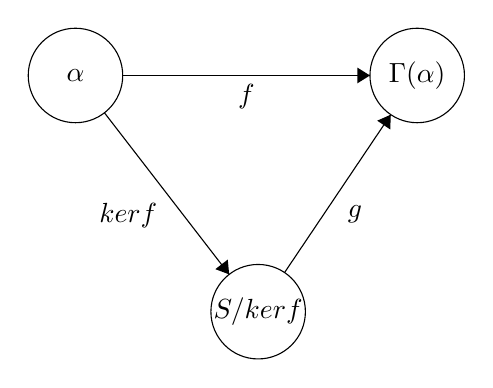
\begin{tikzpicture}[scale=0.2] \tikzstyle{every node}+=[inner sep=0pt] \draw [black] (22.1,-16.4) circle (3); \draw (22.1,-16.4) node {$\alpha$}; \draw [black] (43.8,-16.4) circle (3); \draw (43.8,-16.4) node {$\Gamma(\alpha)$}; \draw [black] (33.7,-31.4) circle (3); \draw (33.7,-31.4) node {$S/kerf$}; \draw [black] (35.38,-28.91) -- (42.12,-18.89); \fill [black] (42.12,-18.89) -- (41.26,-19.27) -- (42.09,-19.83); \draw (39.36,-25.24) node [right] {$g$}; \draw [black] (25.1,-16.4) -- (40.8,-16.4); \fill [black] (40.8,-16.4) -- (40,-15.9) -- (40,-16.9); \draw (32.95,-16.9) node [below] {$f$}; \draw [black] (23.94,-18.77) -- (31.86,-29.03); \fill [black] (31.86,-29.03) -- (31.77,-28.09) -- (30.98,-28.7); \draw (27.33,-25.31) node [left] {$kerf$}; \end{tikzpicture} \end{center}

Per dimostrarlo basta prendere:

$f:\,\alpha\rightarrow\mathcal{P}(\Gamma)$

risulta banale verificare che:

$ker\, f\equiv\sim_{\Gamma}$

e quindi, ricordando che g è iniettiva, risulta banale che:

$|S/\sim_{\Gamma}|\leq\Gamma(\alpha)$

Allora possiamo prendere il modello:

$M^{\Gamma}=(S^{\Gamma},R',V^{\Gamma})$

$R'\subseteq S^{\Gamma}\times S^{\Gamma}$

con R' che soddisfi le seguenti proprietà:

F1) $(\alpha,\,\beta)\in R\implies([\alpha],\,[\beta])\in R'$

F2) $([\alpha],[\beta])\in R'\implies\forall\boxx b\in\Gamma,\,\veraw{\mu}{\alpha}{\boxx b}\implies\veraw{\mu}{\beta}b$

Una relazione che gode delle proprietà F1 e F2 si chiama $\Gamma$-filtrazione
della relazione R.

prendiamo infine:

$V^{\Gamma}:\,\Phi\cap\Gamma\rightarrow\mathcal{P}(S^{\Gamma})$

che gode della seguente proprietà:

presa una formula atomica $A\in\Phi\cap\Gamma$

$\alpha\in V^{\Gamma}(A)\iff\alpha\in V(A)$


\subsection{Teorema}

Esiste almeno una relazione che gode delle proprietà F1 e F2:

$R^{\sigma}\subseteq S^{\Gamma}\times S^{\Gamma}$

così definita:

$([\alpha],[\beta])\in R^{\sigma}\iff\exists\delta\in[\alpha],\eta\in[\beta]\,:\,(\delta,\,\eta)\in R$

La proprietà F1 è dimostrata banalmente.

Dimostriamo F2

Ip) $([\alpha],[\beta])\in R^{\sigma}$, $\boxx{b\in\Gamma}$, $\veraw{\mu}{\alpha}{\boxx b}$

Ts) $R^{\delta}$gode della proprietà F2

supponiamo che:

$\exists\delta,\eta\,:\,\delta R\eta\wedge\delta\in[\alpha]\wedge\eta\in[\beta]$

avremo che:

$\veraw{\mu}{\delta}{\boxx b}$

$\veraw{\mu}{\eta}b$

e quindi:

$\veraw{\mu}{\beta}b$\\



\section{Lemma di Filtrazione}

dato un insieme$\Gamma$ chiuso rispetto alle sottoformule di a, con
$a\in\Gamma$

$\veraw{\mu}{\alpha}{a\iff}\veraw{\mu^{\Gamma}}{\alpha}a$

per ogni $\mu^{\Gamma}$$\Gamma$-filtrazione di $\mu$

Dimostrazione:

Ts) $\veraw{\mu}{\alpha}{a\iff}\veraw{\mu^{\Gamma}}{[\alpha]}a$

Ip) $\mu^{\Gamma}$$\Gamma$-filtrazione di $\mu$

Per induzione sul numero di connettivi di a

Caso Base, n=0:

a non ha connettivi, allora $a\equiv A$

$\veraw{\mu}{\alpha}A\iff\alpha\in V(A)\iff\alpha\in V^{\Gamma}(A)\iff\veraw{\mu^{\Gamma}}{[\alpha]}a$

Ipotesi di induzione: il teorema vale per ogni formula di $\Gamma$
con m<n connettivi.

a può essere:
\begin{enumerate}
\item $\neg b$
\item $b\implies c$
\item $\boxx b$
\end{enumerate}
Caso 1:

$\veraw{\mu}{\alpha}{\neg b}\iff\nonveraw{\mu}{\alpha}b\iff\nonveraw{\mu^{\Gamma}}{[\alpha]}b\iff\veraw{\mu^{\Gamma}}{[\alpha]}{\neg b}$

Caso 2:

$\veraw{\mu}{\alpha}{b\implies c}$ se e solo se $\nonveraw{\mu}{\alpha}b$
oppure $\veraw{\mu}{\alpha}c$

quindi si può affermare

$\nonveraw{\mu}{\alpha}b\iff\nonveraw{\mu^{\Gamma}}{[\alpha]}b$

$\veraw{\mu}{\alpha}c\iff\veraw{\mu^{\Gamma}}{[\alpha]}c$

ma vale almeno una delle due se e solo se

$\veraw{\mu^{\Gamma}}{[\alpha]}{b\implies c}$

Caso 3:

Ip) $\veraw{\mu}{\alpha}{\boxx b}$

Ts) $\veraw{\mu^{\Gamma}}{[\alpha]}{\boxx b}$

Consideriamo la reazione R' avente le proprietà F1 e F2

$\forall[\beta]\,:\,([\alpha],\,[\beta])\in R'\implies\veraw{\mu^{\Gamma}}{[\beta]}b$
-- per F2

allora si può affermare che:

$\veraw{\mu}{\beta}b\implies\veraw{\mu^{\Gamma}}{[\beta]}b\implies\veraw{\mu^{\Gamma}}{[\alpha]}{\boxx b}$

Ip)$\veraw{\mu^{\Gamma}}{[\alpha]}{\boxx b}$

Ts)$\veraw{\mu}{\alpha}{\boxx b}$

$\forall[\beta]\,:\,(\alpha,\,\beta)\in R,\,([\alpha],\,[\beta])\in R'$
--per F1

allora si può affermare che:

$\veraw{\veraw{\mu^{\Gamma}}{[\beta]}b\implies\mu}{\beta}b\implies\veraw{\mu}{\alpha}{\boxx b}$


\section{Determinatezza di K dai Frame Finiti}

La minima logica normale K è determinata dalla classe di tutti i frame
finiti.

Se $a$ ha n sottoformule $a$ è un teorema di K se e solo se A è
valida in tutti i frame con meno di $2^{n}$ mondi. 

$\teoremaDi Ka$ se e solo se $\vera Fa$.\\


Ip)$\teoremaDi Ka$ 

Ts)$\vera Fa$\\


Se $a$ è un teorema di K allora $a$ è valida in tutti i frame (infatti
K è determinata rispetto alla classe di tutti i frame) è a maggior
ragione valida in tutti i frame finiti ed in tutti i frame con meno
di $2^{n}$ mondi.\\


Ip)$\vera Fa$

Ts)$\teoremaDi Ka$\\
\\
Suppongo per assurdo che$\nonTeor Ka$ se e solo se $\nonvera{M^{K}}a$
se e solo se (per il lemma di filtrazione) $\nonvera{(M^{K})^{\Gamma}}a$
il che implica che

in particolare $\nonvera{(F^{K})^{\Gamma}}a$ dove $(F^{K})^{\Gamma}$
è il Frame su cui è costruita la filtrazione del modello canonico
costruito rispetto alla logica $K$ 

Si noti che $(M^{K})^{\Gamma}$ ha al più $2^{n}$ mondi.


\section{Determinatezza di KD dai Frame seriali finiti}

Per seguire lo stesso ragionamente della dimostrazione appena fatta,
dobbiamo solo mostrare che se $R$ è seriale allora $R^{\sigma}$
lo è.\\


\ovalbox{\begin{minipage}[t]{1\columnwidth}%
\textbf{Nota:}$R^{\sigma}\subseteq S^{\Gamma}\times S^{\Gamma}$

così definita:

$([\alpha],[\beta])\in R^{\sigma}\iff\exists\delta\in[\alpha],\eta\in[\beta]\,:\,(\delta,\,\eta)\in R$%
\end{minipage}}\\
\\
Sia $[\alpha]\in S^{\Gamma}$

Se $R^{KD}$ è seriale allora $\forall\delta\in S^{KD}\exists\eta\in S^{KD}:\ (\delta,\eta)\in R^{KD}$

In particolare esiste$\delta$ appartiene alla classe di equivalenza
$[\alpha]$ (di cui al limite potrebbe essere l'unico elemento con
$\alpha=\delta$)

Dalla serialità abbiamo che esiste$\eta$ appartiene alla classe di
equivalenza $[\beta]$

Da cui $([\alpha],[\beta])\in R^{\sigma}$


\section{Determinatezza di K4 dai Frame transitivi finiti}

L'aspetto interessante di questa dimostrazione sta nel fatto che non
possiamo usare la relazione ``classica'' $R^{\sigma}$ come $\Gamma$-filtrazione
ma dobbiamo costruirne una ad hoc, dato che se $R^{K4}$ è transitiva
la sua filtrazione standard non è detto che lo sia

Definiamo quindi $R^{\tau}$così:

$([\alpha],[\beta])\in R^{\tau}$ se se e solo se per ogni fbf $b$,
$\boxx b\in\Gamma$ e $\vera M{_{\alpha}\boxx b}$ implicano $\vera M{_{\beta}b\wedge\boxx b}$

dimostriamo che $R^{\tau}$ è una $\Gamma$-filtrazione transitiva\\


$R^{\tau}$è una $\Gamma$-filtrazione\\


F2) $([\alpha],[\beta])\in R^{\tau}$ se e solo se$\vera M{_{\alpha}\boxx b}$
implicano $\vera M{_{\beta}b\wedge\boxx b}$ da cui: $\{b\ |\ \boxx{b\in\alpha\}\subseteq\beta}$
e quindi $\alpha,\beta\in R^{K4}$

F1) $(\alpha,\beta)\in R^{K4}$per ogni $\boxx{b\in\Gamma}$, se $\vera M{_{\alpha}\boxx b}$
allora anche (schema 4) $\veraw M{\alpha}{\boxx{\boxx b}}$ 

dato che $(\alpha,\beta)\in R^{K4}$ , anche:

$\veraw M{\beta}b$ e $\veraw M{\beta}{\boxx b}$ e quindi:

$\veraw M{\beta}{b\wedge\boxx b}$\\


$R^{\tau}$ è transitiva\\


Sia $([\alpha],[\beta])\in R^{\tau}$, $([\beta],[\gamma])\in R^{\tau}$
ora la prima implica che per ogni fbf $b$, da $\boxx{b\in\Gamma}$
e $\veraw M{\alpha}{\boxx b}$ segua $\vera M{_{\beta}\boxx{b\wedge b}}$,
e da questa essendo $([\alpha],[\beta])\in R^{\tau}$, segue anche
$\vera M{_{\gamma}\boxx{b\wedge b}}$, cioè $([\beta],[\gamma])\in R^{\tau}$


\section{Tableaux}

I Tableaux sono un metodo efficiente per dimostrare la verità, falsità
e soddisfacibilità di una formula

Il metodo consiste nel partire dalla formula che si vuole considerare,
negandola.

Dopodichè si procede passo passo alla costruzione di un albero seguendo
delle regole di espansione che aggiungono uno o più nodi o rami all'albero.

Le regole con la virgola aggiungono un nodo allo stesso ramo, mentre
le regole con il pipe sdoppiano il ramo.

Se espando una formula, devo aggiungere coerentemente l'espansione
a tutti i sottorami, e non posso più espanderla.

Se un cammino contiene sia una formula che la sua negazione il cammino
si chiude.

Se esiste almeno un cammino chiuso, la formula di partenza è soddisfacibile,
se tutti i cammini sono chiusi, la formula è logicamente valita, altrimenti
la formula è falsa.


\subsection{Tableaux per la logica proposizionale}

Le regole Per applicare l'algoritmo dei tableaux nella logica proposizionale
sono le seguenti:
\begin{itemize}
\item Radice dell'albero\\
$\neg a$
\item Regola del $\neg$\\
$\dfrac{\neg\neg a}{a}$
\item Regole di tipo $\alpha$\\
$\dfrac{a\wedge b}{a,\, b}$ $\dfrac{\neg(a\vee b)}{\neg a,\,\neg b}$
$\dfrac{\neg(a\implies b)}{a,\,\neg b}$
\item Regole di tipo $\beta$\\
$\dfrac{a\vee b}{a|b}$ $\dfrac{\neg(a\wedge b)}{\neg a|\neg b}$
$\dfrac{a\implies b}{\neg a|b}$
\item Regole di tipo $\iff$\\
$\dfrac{a\iff b}{a,\, b|\neg a,\,\neg b}$ $\dfrac{\neg(a\iff b)}{a,\,\neg b|\neg a,\, b}$
\end{itemize}

\subsection{Tableaux per le logiche modali}

Per le logiche modali, si può modificare l'algoritmo già usato per
le logiche proposizionali, aggiungendo le regole per la necessitazione
e considerando che ogni regola deve essere vera in un mondo.

Per fare ciò devo aggiungere l'indice del mondo a tutte le regole,
e si potrà chiudere un ramo solo se si trova la regola e il suo negato
nello stesso mondo.

Le regole dei tableaux per le logiche modali saranno:
\begin{itemize}
\item Radice dell'albero\\
$1.\neg a$
\item Regola del $\neg$\\
$\dfrac{\delta\,\neg\neg a}{\delta a}$
\item Regole di tipo $\alpha$\\
$\dfrac{\delta\, a\wedge b}{\delta\, a,\,\delta\, b}$ $\dfrac{\delta\,\neg(a\vee b)}{\delta\,\neg a,\,\delta\,\neg b}$
$\dfrac{\delta\,\neg(a\implies b)}{\delta\, a,\,\delta\,\neg b}$
\item Regole di tipo $\beta$\\
$\dfrac{\delta\, a\vee b}{\delta\, a|\delta\, b}$ $\dfrac{\delta\,\neg(a\wedge b)}{\delta\,\neg a|\delta\,\neg b}$
$\dfrac{\delta\, a\implies b}{\delta\,\neg a|\delta\, b}$
\item Regole di tipo $\iff$\\
$\dfrac{\delta\, a\iff b}{\delta\, a,\,\delta\, b|\delta\,\neg a,\,\delta\,\neg b}$
$\dfrac{\delta\,\neg(a\iff b)}{\delta\, a,\,\delta\,\neg b|\delta\,\neg a,\,\delta\, b}$
\item Regole di necessitazione\\
$\dfrac{\sigma\,\boa}{\sigma_{n}\, a}$ $\dfrac{\sigma\,\neg\dia}{\sigma_{n}\,\neg a}$
-- con $\sigma_{n}$ già presente nei nodi precedenti\\
$\dfrac{\sigma\,\neg\boa}{\sigma_{n}\,\neg a}$ $\dfrac{\sigma\,\dia}{\sigma_{n}\, a}$
-- con $\sigma_{n}$ non presente nei nodi precedenti
\end{itemize}
Tuttavia queste regole non sono sufficienti se vogliamo usare una
regola modale differente da K.

Per lavorare su regole con proprietà dei frame particolari, devo necessariamente
cambiare le regole di necessitazione aggiungendo dei vincoli alla
generazione di nuovi mondi in modo tale che rispettino le proprietà
del frame.


\section{Logiche notevoli}

Abbiamo visto K essere la logica modale minima, a partire da questa
logica ne possiamo ottenere altre aggiungendo ad essa alcuni schemi
di assiomi:
\begin{itemize}
\item D : $\boa\implies\dia$ (seriale)
\item T: $\boa\implies a$ (riflessiva)
\item B: $a\implies\boxx{\dia}$ (simmetrica)
\item 4:$\boa\implies\boxx{\boa}$ (transitiva)
\item 5: $\diam a\implies\boxx{\diam a}$ (euclidea)
\end{itemize}
Per ognuno di questi schemi di assiomi (X) ne esiste il cosiddetto
duale (X$\diamond$), cioè lo schema che si ottine invertendo antecedente
e conseguente e negando $\boxx a$ con $\dia$


\subsection{Teorema: validità del duale }

M sia una sequenza di connettivi $\square$, $\diamond$ ed M' il
suo duale.

Idem per N ed N'.\\


Ip) $Ma\implies Nb$

Ts) $N'b\implies M'a$\\


Se vale lo schema d'assiomi $Ma$ deve valere anche $M\neg a$ dato
che appunto è uno schema.

Riscrivo l'ipotesi come:

$M\neg a\implies N\neg b$

Considero la tautologia della PL: $(C\implies D)\implies(\neg D\implies\neg C)$

la applico all'ipotesi ottenendo:

$(M\neg a\implies N\neg b)\implies(\neg(N\neg b)\implies\neg(M\neg a))$

Da cui per MP con l'ipotesi (riscritta) ottengo:

$\neg(N\neg b)\implies\neg(M\neg a)$

Usando ripetutamente le equivalenze tra$\square$ e $\diamond$ ottengo:

$N'\neg\neg b\implies M'\neg\neg a$ semplificando:

$N'b\implies M'a$

La dimostrazione nell'altro senso è del tutto simmetrica dato che
le operazioni effettuate sono valide in entrambe le direzioni


\subsection{Esempio validità del duale: schema 5}

Ip) $\diam a\implies\boxx{\diam a}$

Ts)$\diamond\boxx a\implies\boxx a$\\


Riscrivo l'ipotesi come:

$\diam{\neg a}\implies\boxx{\diam{\neg a}}$

Considero la tautologia della PL: $(C\implies D)\implies(\neg D\implies\neg C)$

$(\diam{\neg a}\implies\boxx{\diam{\neg a}})\implies(\neg\boxx{\diam{\neg a}}\implies\neg\diam{\neg a})$

Semplifico il conseguente :$\neg\boxx{\diam{\neg a}}\implies\neg\diam{\neg a}$
diventa

$\diam{\square\neg\neg a\implies\square\neg\neg a}$ , semplificando
i $\neg$:

$\diam{\square a\implies\square a}$

Cioè la tesi.\\


Vogliamo ora mostrare come alcune notazione della forma KX denotino
la stessa logica.

Ricordiamo che con KX intendiamo la logica K a cui abbiamo aggiunto
il generico assioma X

KB4 = K + assioma B + assioma 4


\subsection{Inclusione di KD in KT}

Pare ovvio che una logica riflessiva sia anche seriale (se parlo da
solo parlo con qualcuno), ma dimostriamolo comunque. \\


Ip) KT

Ts) KD\\
Se vale T: 

$\boa\implies a$ (riflessiva)

allora vale anche il suo duale $T\diamond$:

$a\implies\dia$

Per la catena di implicazioni $(\implica ab,\ \implica bc,\ \mbox{\ensuremath{\implica ac}})$
abbiamo:

$\boa\implies\dia$

Cioè lo schema D\\


\textbf{Lemma implica in KB:}

IP)$\teoremaDi{KB}\diamond C\implies D$

TS) $\teoremaDi{KB}\implica C{\boxx D}$\\


Per Ip) $\diamond C\implies D$ e quindi, dato che è un teorema della
logica KB, (che è una logica normale)

posso usare la definizione 3 equivalente di logica normale ottenendo:

$\square\diamond C\implies\square D$ 

Inoltre vale lo schema B

$C\implies\boxx{\diam C}$

Leggendo i due schemi appena scritti dal secondo al primo riconosciamo
la catena di implicazioni $(\implica ab,\ \implica bc,\ \mbox{\ensuremath{\implica ac}})$ 

Da cui: $C\implies\boxx D$


\subsection{Equivalenza KB4, KB5}

\textbf{Da KB4 a KB5}

Valendo 4 vale anche 4$\diamond$:

$\diamond(\dia)\implies(\diamond a)$, e tenendo conto del precedente
lemma 

(dove $C$ è $\diamond a$ e $B$ è $\diamond a$), 

abbiamo $\diamond a\implies\boxx{\dia}$ cioè lo schema5. \\


\textbf{Da KB5 a KB4}

Da 5 infatti deduciamo 5$\diamond$: $\diam{(\square a)\implies(\boa)}$

Tenuto conto della prima osservazione (con$C$ e$B$ uguali ad $a$)

abbiamo $\boa\implies\boxx{\boa}$.\\



\subsection{Equivalenza KDB4. KDB5, KDB45, KTB4, KT5}

\textbf{KDB4 = KDB5 = KD45}, infatti aggiungendo l'assioma D a due
logiche equivalenti (KB4, KB5) continuano a rimanere equivalenti;

aggiungere 4 a KDB5 non produce alcun effetto perché lo contiene già.\\


Inoltre notiamo che: \textbf{KDB4$\subseteq$KTB4} in quanto KT contiene
KD

e \textbf{KT5$\subseteq$KTB4} in quando KT4B contiene KT4 che coincide
con KT5.\\


Mostriamo che \textbf{KTB4$\mbox{\ensuremath{\subseteq}}$KDB4 }così
da arrivare a KTB4 = KDB4

Cioe' mostriamo che nella logica K, dall'assioma T, con B e 4 posso
dedurre l'assioma D

Dall'assioma T deduciamo l'assioma T$\diamond$ cioe' $a\implies\diamond a$

Dato che vale 5: $\diam a\implies\boxx{\diam a}$, sfruttando la catena
di implicazioni delle due precedenti abbiamo:

$a\implies\boxx{\dia}$ cioè B.\\



\subsection{Reticolo delle logiche}

\begin{center} 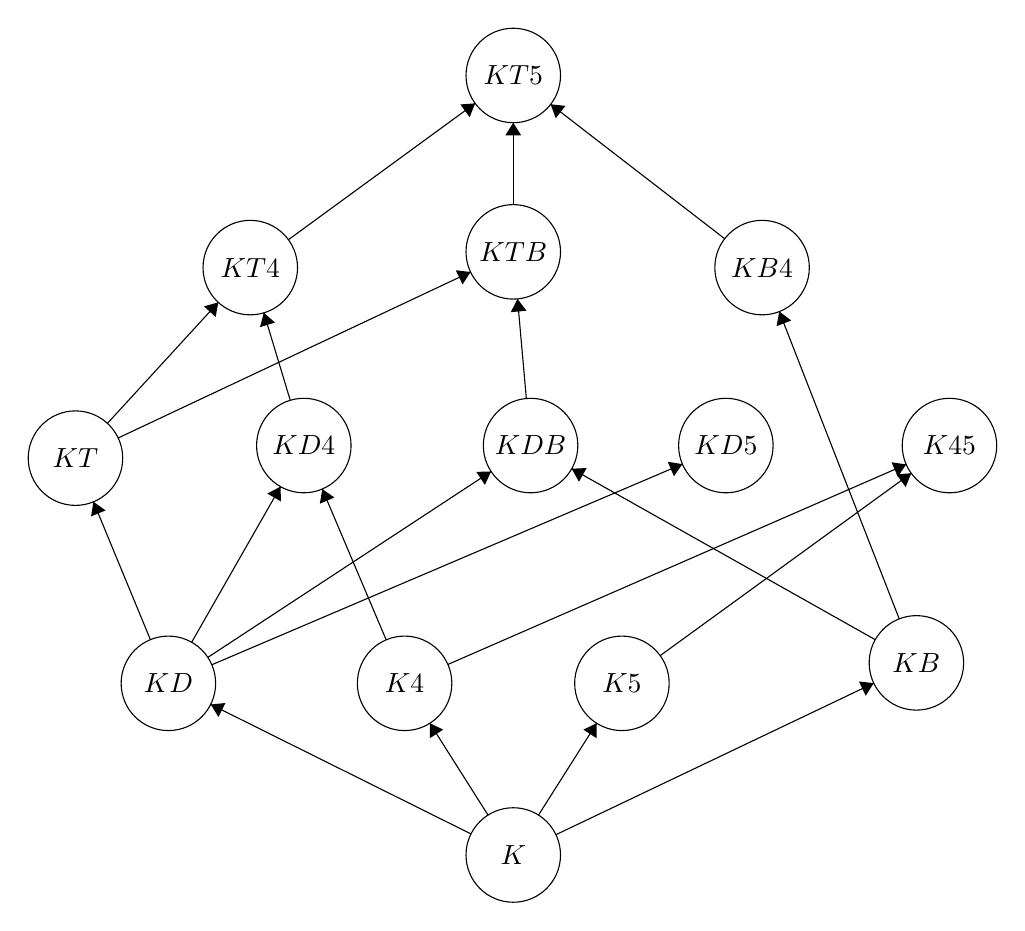
\begin{tikzpicture}[scale=0.2] \tikzstyle{every node}+=[inner sep=0pt] \draw [black] (39.9,-53.7) circle (3); \draw (39.9,-53.7) node {$K$}; \draw [black] (18,-42.8) circle (3); \draw (18,-42.8) node {$KD$}; \draw [black] (33,-42.8) circle (3); \draw (33,-42.8) node {$K4$}; \draw [black] (65.5,-41.5) circle (3); \draw (65.5,-41.5) node {$KB$}; \draw [black] (46.8,-42.8) circle (3); \draw (46.8,-42.8) node {$K5$}; \draw [black] (12.1,-28.5) circle (3); \draw (12.1,-28.5) node {$KT$}; \draw [black] (26.6,-27.7) circle (3); \draw (26.6,-27.7) node {$KD4$}; \draw [black] (53.4,-27.7) circle (3); \draw (53.4,-27.7) node {$KD5$}; \draw [black] (67.6,-27.7) circle (3); \draw (67.6,-27.7) node {$K45$}; \draw [black] (23.2,-16.4) circle (3); \draw (23.2,-16.4) node {$KT4$}; \draw [black] (39.9,-15.4) circle (3); \draw (39.9,-15.4) node {$KTB$}; \draw [black] (55.7,-16.4) circle (3); \draw (55.7,-16.4) node {$KB4$}; \draw [black] (39.9,-4.2) circle (3); \draw (39.9,-4.2) node {$KT5$}; \draw [black] (41,-27.7) circle (3); \draw (41,-27.7) node {$KDB$}; \draw [black] (37.21,-52.36) -- (20.69,-44.14); \fill [black] (20.69,-44.14) -- (21.18,-44.94) -- (21.62,-44.05); \draw [black] (38.3,-51.17) -- (34.6,-45.33); \fill [black] (34.6,-45.33) -- (34.61,-46.28) -- (35.45,-45.74); \draw [black] (42.61,-52.41) -- (62.79,-42.79); \fill [black] (62.79,-42.79) -- (61.85,-42.68) -- (62.28,-43.59); \draw [black] (41.5,-51.17) -- (45.2,-45.33); \fill [black] (45.2,-45.33) -- (44.35,-45.74) -- (45.19,-46.28); \draw [black] (16.86,-40.03) -- (13.24,-31.27); \fill [black] (13.24,-31.27) -- (13.09,-32.2) -- (14.01,-31.82); \draw [black] (14.13,-26.29) -- (21.17,-18.61); \fill [black] (21.17,-18.61) -- (20.26,-18.86) -- (21,-19.54); \draw [black] (25.74,-24.83) -- (24.06,-19.27); \fill [black] (24.06,-19.27) -- (23.82,-20.18) -- (24.77,-19.89); \draw [black] (31.83,-40.04) -- (27.77,-30.46); \fill [black] (27.77,-30.46) -- (27.62,-31.39) -- (28.54,-31); \draw [black] (19.48,-40.19) -- (25.12,-30.31); \fill [black] (25.12,-30.31) -- (24.28,-30.75) -- (25.15,-31.25); \draw [black] (20.76,-41.62) -- (50.64,-28.88); \fill [black] (50.64,-28.88) -- (49.71,-28.73) -- (50.1,-29.65); \draw [black] (35.75,-41.6) -- (64.85,-28.9); \fill [black] (64.85,-28.9) -- (63.92,-28.76) -- (64.32,-29.68); \draw [black] (49.23,-41.04) -- (65.17,-29.46); \fill [black] (65.17,-29.46) -- (64.23,-29.53) -- (64.82,-30.34); \draw [black] (64.41,-38.71) -- (56.79,-19.19); \fill [black] (56.79,-19.19) -- (56.62,-20.12) -- (57.55,-19.76); \draw [black] (62.89,-40.03) -- (43.61,-29.17); \fill [black] (43.61,-29.17) -- (44.07,-30) -- (44.56,-29.13); \draw [black] (20.51,-41.15) -- (38.49,-29.35); \fill [black] (38.49,-29.35) -- (37.55,-29.37) -- (38.1,-30.2); \draw [black] (14.81,-27.22) -- (37.19,-16.68); \fill [black] (37.19,-16.68) -- (36.25,-16.57) -- (36.68,-17.47); \draw [black] (40.73,-24.71) -- (40.17,-18.39); \fill [black] (40.17,-18.39) -- (39.74,-19.23) -- (40.74,-19.14); \draw [black] (25.62,-14.63) -- (37.48,-5.97); \fill [black] (37.48,-5.97) -- (36.54,-6.04) -- (37.13,-6.85); \draw [black] (39.9,-12.4) -- (39.9,-7.2); \fill [black] (39.9,-7.2) -- (39.4,-8) -- (40.4,-8); \draw [black] (53.33,-14.57) -- (42.27,-6.03); \fill [black] (42.27,-6.03) -- (42.6,-6.92) -- (43.21,-6.13); \end{tikzpicture} \end{center}

\textbf{\large{Somma diretta di Frame}}\textbf{}\\


S5 è determinata dalla classe dei frame d’ equivalenza (cioè frame
in cui la relazione di accessibilità è una relazione di equivalenza),
S5 = KT5 = KTB4 (riflessiva, simmetrica, transitiva)

S5 è determinata dalla classe dei frame universali (cioè frame in
cui la relazione di accessibilità è la relazione universale).

Mostriamo (almeno argomentiamo) la seconda affermazione.\\


Data una collezione di frame con insiemi di mondi a due a due disgiunti,
si dice somma diretta di questi frame il frame che ha come insieme
dei mondi l’unione dell’insieme dei mondi dei frame della collezione
e come relazione la unione delle relazioni dei frame della collezione.

$F=(S,R)$

$F1=(S1,R1)$, $F2=(S2,R2)$

$F=F1\oplus F2$ se e solo se $F=(S1\cup S2,\ R1\cup R2)$

Si dimostra che $\vera Fa$ se e solo se $\vera{F1}a$ e $\vera{F2}a$

Dato che una relazione di equivalenza forma una partizione sull'insieme
su cui è definita, e che in ogni classe di equivalenza è una relazione
universale, possiamo vedere una relazione di equivalenza come somma
di relazioni universali e il suo insieme come somma disgiunta di insiemi;
la somma diretta pertanto ci mostra quindi che S5 è determinata dai
frame universali.


\subsection{Tableau rivisitato per KT, KB}

Se una logica contiene l'assioma B devo aggiungere alle regole del
Tableau
\begin{itemize}
\item Regole di necessitazione\\
$\dfrac{\sigma\,\boa}{\sigma_{n}\, a}$ $\dfrac{\sigma\,\neg\dia}{\sigma_{n}\,\neg a}$
-- con $\sigma_{n}$ già presente nei nodi precedenti, oppure $\sigma_{n}$
\textbf{nodo corrente}
\end{itemize}
es. Si provi che la formula: $(\boa\implies a)$ è un teorema in KB

1: $\neg(\boa\implies a)$

1: $\boa$

1: $\neg a$

\textbf{1}: $a$ 

\begin{center}
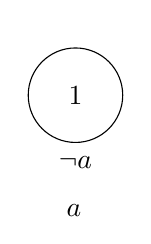
\begin{tikzpicture}[scale=0.2] 
\tikzstyle{every node}+=[inner sep=0pt] 
\draw [black] (26.8,-10.8) circle (3);
\draw (26.8,-10.8) node {1}; 

 
\draw (26.8,-6.6) node {$\boa$}; 

\draw (26.8,-15.1) node {$\neg{a}$};

\draw (26.7,-18.1) node {$a$}; 


\end{tikzpicture}
\end{center} 

Dove nell'ultimo passaggio ho usato proprio la regola appena introdotta,
avendo ottenuto $a$ e $\neg a$ nello stesso stato (mondo) deduco
che negare $a$ mi porta a un assurdo e quindi deve per forza essere
un teorema.\\
Se una logica contiene l'assioma T devo aggiungere alle regole del
Tableau
\begin{itemize}
\item Regole di necessitazione

\begin{itemize}
\item $\dfrac{\sigma\,\boa}{\sigma_{n}\, a}$ $\dfrac{\sigma\,\neg\dia}{\sigma_{n}\,\neg a}$
-- con $\sigma_{n}$ già presente nei nodi precedenti, oppure $\sigma_{n}$
\textbf{nodo prefisso del nodo corrente} (es 11 è prefisso di 111)
\end{itemize}
\end{itemize}
es. Si provi che la formula $(a\implies\boxx{\diamond a})$ è un teorema
in KT

1:$\neg(a\implies\boxx{\diamond a})$

1:$a$

1:$\neg(\boxx{\dia})$

1: $\diamond\boxx{\neg a}$

11: $\boxx{\neg a}$

\textbf{1: $\neg a$}

\begin{center} 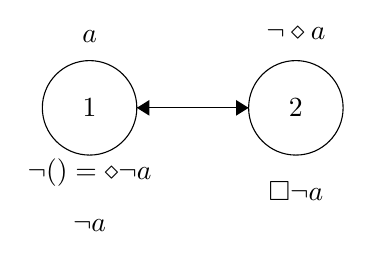
\begin{tikzpicture}[scale=0.2] \tikzstyle{every node}+=[inner sep=0pt] \draw [black] (26.7,-10.8) circle (3); \draw (26.7,-10.8) node {$1$};
\draw (26.7,-14.9) node {$\neg(\boxx{\dia})=\diamond\boxx{\neg a}$};
\draw (26.7,-18.3) node {$\neg a$}; \draw [black] (39.8,-10.8) circle (3); \draw (39.8,-10.8) node {$2$};
\draw (26.7,-6.3) node {$a$};
\draw (39.8,-6.1) node {$\neg\diamond a$};
\draw (39.8,-16.1) node {$\square\neg a$}; \draw [black] (29.7,-10.8) -- (36.8,-10.8); \fill [black] (36.8,-10.8) -- (36,-10.3) -- (36,-11.3); \draw [black] (36.8,-10.8) -- (29.7,-10.8); \fill [black] (29.7,-10.8) -- (30.5,-11.3) -- (30.5,-10.3); \end{tikzpicture} \end{center}




\chapter{	Logica temporale}


\section{Sottomodello generato da $\alpha$}

presa una logica $\Lambda$ e un modello $\mu=(S,\, R,\, V)$, prendiamo
un qualunque $\alpha\in S$

Si dice sottomodello generato da $\alpha$ il modello:

$\mu^{\alpha}=(S^{\alpha},\, R^{\alpha},\, V^{\alpha})$

con:

$S^{\alpha}=\{\beta\,|\,\alpha R*\beta\}$ dove R{*} è la chiusura
riflessiva e transitiva di R

$R^{\alpha}\subseteq S^{\alpha}\times S^{\alpha}$

$R^{\alpha}=R\,\cap\, S^{\alpha}\times S^{\alpha}$

e la valutazione tale che:

$\beta\in V^{\alpha}(A)\iff\beta\in S^{\alpha}\wedge\beta\in V(A)$


\subsection{Lemma}

Ip) $\beta\in S^{\alpha}$

Ts) $\veraw{\mu}{\beta}a\iff\veraw{\mu^{\beta}}{\beta}a$\\
Dimostrazione per induzione sulla complessità di a:

Caso base: $a\in\Phi$

$\beta\in V(a)\implies\beta\in V^{\alpha}(a)$

Ipotesi di induzione: il teorema vale per formule con un numero di
connettivi minore di n.

Bisogna dimostrare 3 casi:

1) $\neg b$

2) $b\implies c$

3) $\boxx b$

i primi due casi sono banali, come negli altri casi. Dimostriamo l'ultimo.

Ip) $\veraw{\mu^{\alpha}}{\beta}{\boxx b}$ 

Ts) $\veraw{\mu}{\beta}{\boxx b}$

$\veraw{\mu^{\alpha}}{\beta}{\boxx b\iff\veraw{\mu^{\alpha}}{\gamma}b}$,
per ogni $\gamma$ tale che $\beta R^{\alpha}\gamma$

ma per ipotesi di induzione:

$\veraw{\mu^{\alpha}}{\gamma}b\iff\veraw{\mu}{\gamma}b\iff\veraw{\mu}{\beta}{\boxx b}$

Ip) $\veraw{\mu}{\beta}{\boxx b}$

Ts) $\veraw{\mu^{\alpha}}{\beta}{\boxx b}$

Per ogni $\delta$ tale che $\beta R^{\alpha}\delta$

si ha che $\beta R\delta$

infatti $R^{\alpha}=R\cap S^{\alpha}\times S^{\alpha}$ e quindi se
$(\beta,\delta)\in R^{\alpha}$ deve essere anche $(\beta,\delta)\in R$

Dall'ipotesi $\veraw{\mu}{\beta}{\boxx b}$, sappiamo che $b$ è vera
in tutti i $\gamma$ tali che $(\beta,\gamma)\in R$ cioè $\vera{\mu}{_{\gamma}b}$,
ma per ipotesi induttiva si ha anche $\vera{\mu^{\alpha}}{_{\gamma}b}$

Da cui la tesi.


\subsection{Corollario}

Valgono le seguenti:

$\vera{\mu}a\implies\vera{\mu^{\alpha}}a$

$\vera{\mu}a\iff\vera{\mu^{\alpha}}a\,\forall\alpha\in S$

$\vera Fa\iff\vera{F^{\alpha}}a\,\forall\alpha\in S$


\section{p-Morfismo}

siano $F_{1}(S_{1},\, R_{1}),\, F_{2}(S_{2},\, R_{2})$ frame.

c'è un p-morfismo (pseudo-morfismo) tra $F_{1}$ e $F_{2}$ se esiste
una applicazione che gode delle seguenti proprietà:

1) $(\alpha,\,\beta)\in R_{1}\implies(f(\alpha),\, f(\beta))\in R_{2}$

2) $(f(\alpha),\,\eta)\in R_{2}\implies\exists\beta\in S_{1}\,:\, f(\beta)=\eta\,\wedge\,(\alpha,\,\beta)\in R_{1}$

Considerati poi due modelli $M_{1}(F_{1},\, V_{1}),\, M_{2}(F_{2},\, V_{2})$,
esiste un p-morfismo tra $M_{1}$ e $M_{2}$se vale la proprietà:

3) $\alpha\in V_{1}(A)\iff f(\alpha)\in V_{2}(A)$

se f è suriettiva, allora il p-morfismo si dice suriettivo


\subsection{Lemma}

Siano $\mu_{1}$ e $\mu_{2}$ due modelli e f un p-morfismo di $\mu_{1}$
su $\mu_{2}$, allora: 

$\veraw{\mu_{1}}{\alpha}a\iff\veraw{\mu_{2}}{f(\alpha)}a$\\
Siano $F_{1}$e $F_{2}$ due frame e f un p-morfismo suriettivo di
$F_{1}$su $F_{2}$, allora:

$\vera{F_{1}}a\implies\vera{F_{2}}a$


\section{Frame ($\omega$, <)}

Il frame ($\omega$, <) è il frame che rappresenta la retta dei numeri
naturali.

E' adatto a rappresentare il tempo discreto continuocon un istante
iniziale.

La logica che rappresenta questo frame è la logica K4DLZ, che è corretta
e completa rispetto a ($\omega$, <)

\begin{center} 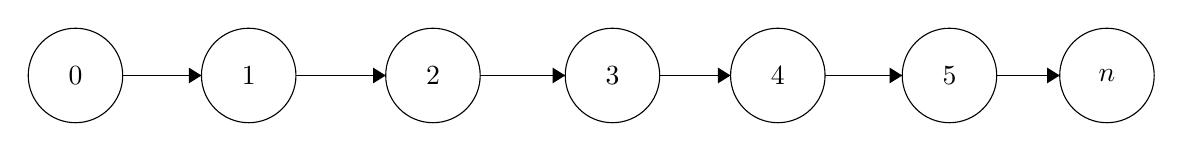
\begin{tikzpicture}[scale=0.2] \tikzstyle{every node}+=[inner sep=0pt] \draw [black] (17.5,-22.3) circle (3); \draw (17.5,-22.3) node {$1$}; \draw [black] (6.5,-22.3) circle (3); \draw (6.5,-22.3) node {$0$}; \draw [black] (29.2,-22.3) circle (3); \draw (29.2,-22.3) node {$2$}; \draw [black] (40.6,-22.3) circle (3); \draw (40.6,-22.3) node {$3$}; \draw [black] (51.1,-22.3) circle (3); \draw (51.1,-22.3) node {$4$}; \draw [black] (62,-22.3) circle (3); \draw (62,-22.3) node {$5$}; \draw [black] (72,-22.3) circle (3); \draw (72,-22.3) node {$n$}; \draw [black] (9.5,-22.3) -- (14.5,-22.3); \fill [black] (14.5,-22.3) -- (13.7,-21.8) -- (13.7,-22.8); \draw [black] (20.5,-22.3) -- (26.2,-22.3); \fill [black] (26.2,-22.3) -- (25.4,-21.8) -- (25.4,-22.8); \draw [black] (32.2,-22.3) -- (37.6,-22.3); \fill [black] (37.6,-22.3) -- (36.8,-21.8) -- (36.8,-22.8); \draw [black] (43.6,-22.3) -- (48.1,-22.3); \fill [black] (48.1,-22.3) -- (47.3,-21.8) -- (47.3,-22.8); \draw [black] (54.1,-22.3) -- (59,-22.3); \fill [black] (59,-22.3) -- (58.2,-21.8) -- (58.2,-22.8); \draw [black] (65,-22.3) -- (69,-22.3); \fill [black] (69,-22.3) -- (68.2,-21.8) -- (68.2,-22.8); \end{tikzpicture} \end{center}


\section{La logica K4DLZ}

la logica K4DLZ, detta anche logica $\Omega$ è la logicha che ha,
oltre all'assioma K, i seguenti assiomi:
\begin{itemize}
\item 4: $\boa\implies\boxx{\boa}$ --> transitività
\item D: $\boa\implies\dia$ --> serialità
\item L: $\boxx{(a\wedge\boa\implies b)}\vee\boxx{(b\wedge\boxx b\implies a)}$
--> debole connessione
\item Z: $\boxx{(\boa\implies a)\implies(\diam{\boa}\implies\boa)}$
\end{itemize}
L'azssioma Z, non ha alcuna interpretazione preso a se stante, ma
in combinazione con gli altri implica che tra due mondi connessi c'è
solo un numero finito di mondi, a due a due connessi.


\section{Correttezza di K4DLZ}

Ip) $\teolm{\Omega}a$

Ts) $\vera{(\omega,<)}a$

Per dimostrare questo teorema dobbiamo dimostrare che ogni teorema
di K4DLZ è una formula valida. Poichè ogni teorema di $\Omega$ è
una serie di applicazioni degli assiomi o delle regole di inferenza,
dobbiamo assicurare che:
\begin{enumerate}
\item Modus Ponens e la regola di necessitazione fanno passare da formule
valide a formule valide. Come abbiamo dimostrato, questo è sempre
vero.
\item Gli assiomi siano formule valide:\end{enumerate}
\begin{itemize}
\item A1, A2, A3, K sono validi su ogni frame, e quindi sono validi anche
su ($\omega$, <)
\item 4 è valido su ogni frame transitivo, e quindi è valido anche su ($\omega$,
<) essendo transitivo
\item D è valido su ogni frame seriale, e quindi è valido anche su ($\omega$,
<) essendo seriale.
\item L è valido su ogni frame debolmente connesso, e quindi è valido anche
su ($\omega$, <) essendo debolmente connesso.\\

\end{itemize}
Dobiamo quindi dimostrare solo la validità di Z.

Z è l'assioma $\boxx{(\boa\implies a)\implies(\diam{\boa}\implies\boa)}$,
per dimostrare che è valido basta considerare il caso in cui gli antecedenti
delle implicazioni siano validi

supponiamo dunque che esistano due mondi $\alpha$ e $\beta$ con
$\alpha<\beta$ tali che

$\veraw{(\omega,\,<)}{\alpha}{\boxx{(\boa\implies a)}}$

$\veraw{(\omega,\,<)}{\alpha}{\diam{\boa}}$

$\veraw{(\omega,\,<)}{\beta}{\boa}$

allora da quest'ultima, viste le altre proprietà del frame, $\forall\eta>\beta$
avremo:

$\veraw{(\omega,\,<)}{\eta}a$

dalla prima invece abbiamo:

$\veraw{(\omega,\,<)}{\beta}{\boa\implies a}$

e allora, applicando il modus ponens

$\veraw{(\omega,\,<)}{\beta}a$

Ma, allora possiamo applicare lo stesso ragionamento per $\beta-1$,
poichè:

$\veraw{(\omega,\,<)}{\beta-1}{\boa}$

\begin{center} 
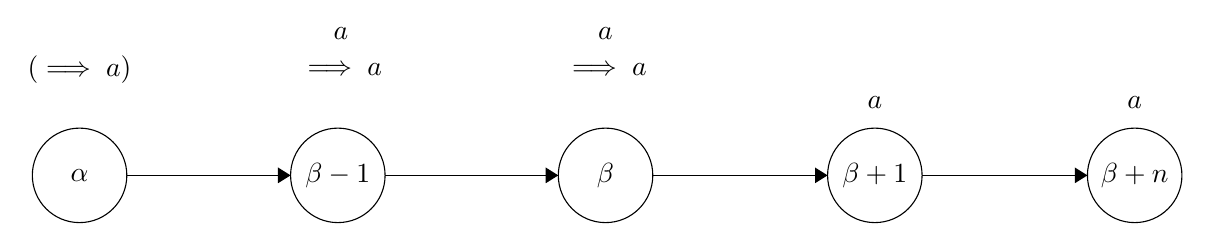
\begin{tikzpicture}[scale=0.2] 
\tikzstyle{every node}+=[inner sep=0pt] 
\draw [black] (6.1,-28.6) circle (3); 
\draw (6.1,-28.6) node {$\alpha$}; 
\draw [black] (22.5,-28.6) circle (3); 
\draw (22.5,-28.6) node {$\beta-1$}; 
\draw [black] (56.6,-28.6) circle (3); 
\draw (56.6,-28.6) node {$\beta+1$}; 
\draw [black] (73.1,-28.6) circle (3); 
\draw (73.1,-28.6) node {$\beta+n$}; 
\draw [black] (39.5,-28.6) circle (3); 
\draw (39.5,-28.6) node {$\beta$}; 
\draw (73.1,-24) node {$a$}; 
\draw (56.6,-24) node {$a$}; 
\draw (39.5,-24) node {$\boa$}; 
\draw (39.5,-21.9) node {$\boa\implies a$}; 
\draw (39.5,-19.6) node {$a$}; 
\draw (6.1,-24.6) node {$\diam{\boa}$}; 
\draw (6.1,-21.9) node {$\boxx{(\boa\implies a)}$}; 
\draw (22.5,-24) node {$\boa$}; 
\draw (22.7,-21.9) node {$\boa\implies a$}; 
\draw (22.7,-19.6) node {$a$}; 
\draw [black] (9.1,-28.6) -- (19.5,-28.6); 
\fill [black] (19.5,-28.6) -- (18.7,-28.1) -- (18.7,-29.1); 
\draw [black] (59.6,-28.6) -- (70.1,-28.6); 
\fill [black] (70.1,-28.6) -- (69.3,-28.1) -- (69.3,-29.1); 
\draw [black] (42.5,-28.6) -- (53.6,-28.6); 
\fill [black] (53.6,-28.6) -- (52.8,-28.1) -- (52.8,-29.1); 
\draw [black] (25.5,-28.6) -- (36.5,-28.6); 
\fill [black] (36.5,-28.6) -- (35.7,-28.1) -- (35.7,-29.1);
\end{tikzpicture} 
\end{center}

Ma, siccome esiste un numero finito di mondi tra $\alpha$ e $\beta$,
arriveremo a un certo punto a provare che:

$\veraw{(\omega,\,<)}{\alpha+1}a$

e quindi:

$\veraw{(\omega,\,<)}{\alpha}{\boa}$

\begin{center} 
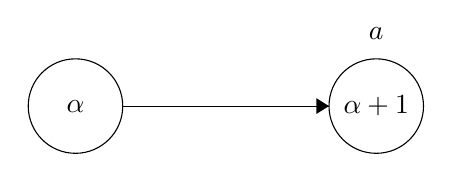
\begin{tikzpicture}[scale=0.2] 
\tikzstyle{every node}+=[inner sep=0pt] 
\draw [black] (28,-22.8) circle (3); 
\draw (28,-22.8) node {$\alpha$}; 
\draw [black] (47.1,-22.8) circle (3); 
\draw (47.1,-22.8) node {$\alpha+1$}; 
\draw (47.1,-18.2) node {$a$}; 
\draw (27.9,-18.6) node {$\boa$}; 
\draw [black] (31,-22.8) -- (44.1,-22.8); 
\fill [black] (44.1,-22.8) -- (43.3,-22.3) -- (43.3,-23.3); 
\end{tikzpicture} 
\end{center}

e la tesi è dimostrata.


\section{Completezza di K4DLZ}

Ip) $\vera{(\omega,<)}a$

Ts)$\teolm{\Omega}a$ 

Questa dimostrazione è così lunga da essere suddivisa per convenienza
in punti

\textbf{1)}

Per assurdo supponiamo che non valga la tesi, cioè che 

$\nonTeor{\Omega}a$, per il lemma di verità si ha anche $\nonvera{M^{\Omega}}a$,
$M^{\Omega}=M_{1}$

$M_{1}$è seriale, transitivo e debolmente connesso, infatti queste
proprietà si conservano quando si passa dalla logica al modello canonico.

Dato che $\nonvera{M^{\Omega}}a$, in particolare esiste un mondo
$\alpha$ in cui $\nonveraw{M_{1}}{\alpha}a$

\textbf{2)}

$M_{2}=M_{1}^{\alpha}$, dove $M_{1}^{\alpha}$ è il sottomodello
genereato da $\alpha$.

$M_{2}$ è seriale, transitivo e connesso. La serialità e la transitività
vengono direttamente da $M_{1}$, esaminiamo la connessione.

$M_{2}=(S_{2},R_{2},V_{2})$ se $\delta\in S_{2}$e $\gamma\in S_{2}$
allora $(\alpha,\gamma)\in R_{1}^{*}$ e $(\alpha,\delta)\in R_{1}^{*}$

Dato che $R_{1}$è già transitiva(vedi punto 1) la sua chiusura riflessiva
e transitiva si limita a unire la relazione identica (cioè aggiunge
gli autoanelli ai mondi)

Dal momento che $R_{1}$ è debolmente connessa, $R_{1}$, avendo anche
la riflessività è connessa.

Inoltre $\nonvera{M_{2}}a$, infatti sappiamo che se $\vera Ma$ allora
$\vera{M^{\alpha}}a$ per ogni mondo $\alpha$ di $M$

\textbf{3)}

$M^{3}=$$\Gamma$-filtrazione di $M_{2}$, con $\Gamma=Stf(a)$

dove come $\Gamma$-filtrazione delle relazione di raggiungibilità
di $M_{2}$ si prende la filtrazione transitiva. 

$M^{3}$ è ancora seriale e connesso ed è transitivo per costruzione,
inoltre il suo insieme di mondi ha cardinalità limitata superiormente
da $2^{|Sfm(A)|}$

Inoltre $\nonvera{M_{3}}a$

\textbf{4-pre)}

Diciamo palloncino un frame $(T,\rho)$ dove 

$T=\{\alpha_{1},\alpha_{2},...,\alpha_{n},\alpha_{n+1},...,\alpha_{n+m}\}$
e 

$i.j\in\rho\ \iff\ i<j\ oppure\ i,j\geq n$ 

Sostanzialmente il grafo di $\rho$ si presenta nella seguente forma
(a meno degli archi che esprimono il fatto che $\rho$ è transitiva).\\


\begin{center} 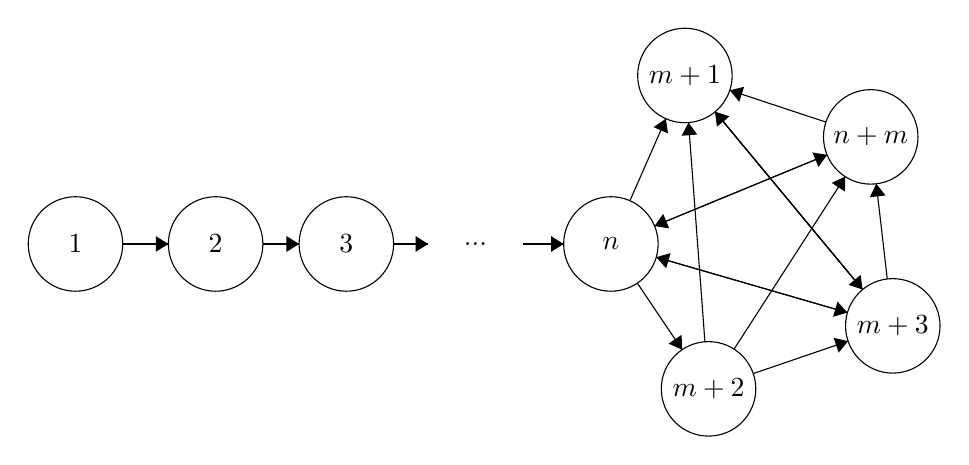
\begin{tikzpicture}[scale=0.2] \tikzstyle{every node}+=[inner sep=0pt] \draw [black] (5.5,-30.4) circle (3); \draw (5.5,-30.4) node {$1$}; \draw [black] (14.4,-30.4) circle (3); \draw (14.4,-30.4) node {$2$}; \draw [black] (22.7,-30.4) circle (3); \draw (22.7,-30.4) node {$3$}; \draw [black] (39.5,-30.4) circle (3); \draw (39.5,-30.4) node {$n$}; \draw [black] (44.2,-19.7) circle (3); \draw (44.2,-19.7) node {$m+1$}; \draw [black] (45.7,-39.6) circle (3); \draw (45.7,-39.6) node {$m+2$}; \draw [black] (57.4,-35.6) circle (3); \draw (57.4,-35.6) node {$m+3$}; \draw [black] (56,-23.6) circle (3); \draw (56,-23.6) node {$n+m$};
\draw (30.9,-30.4) node {$...$}; \draw [black] (8.5,-30.4) -- (11.4,-30.4); \fill [black] (11.4,-30.4) -- (10.6,-29.9) -- (10.6,-30.9); \draw [black] (17.4,-30.4) -- (19.7,-30.4); \fill [black] (19.7,-30.4) -- (18.9,-29.9) -- (18.9,-30.9); \draw [black] (40.71,-27.65) -- (42.99,-22.45); \fill [black] (42.99,-22.45) -- (42.21,-22.98) -- (43.13,-23.38); \draw [black] (42.27,-29.26) -- (53.23,-24.74); \fill [black] (53.23,-24.74) -- (52.3,-24.59) -- (52.68,-25.51); \draw [black] (42.38,-31.24) -- (54.52,-34.76); \fill [black] (54.52,-34.76) -- (53.89,-34.06) -- (53.61,-35.02); \draw [black] (41.18,-32.89) -- (44.02,-37.11); \fill [black] (44.02,-37.11) -- (43.99,-36.17) -- (43.16,-36.73); \draw [black] (48.54,-38.63) -- (54.56,-36.57); \fill [black] (54.56,-36.57) -- (53.64,-36.36) -- (53.97,-37.3); \draw [black] (57.05,-32.62) -- (56.35,-26.58); \fill [black] (56.35,-26.58) -- (55.94,-27.43) -- (56.94,-27.32); \draw [black] (53.15,-22.66) -- (47.05,-20.64); \fill [black] (47.05,-20.64) -- (47.65,-21.37) -- (47.96,-20.42); \draw [black] (55.48,-33.29) -- (46.12,-22.01); \fill [black] (46.12,-22.01) -- (46.24,-22.94) -- (47.01,-22.3); \draw [black] (54.52,-34.76) -- (42.38,-31.24); \fill [black] (42.38,-31.24) -- (43.01,-31.94) -- (43.29,-30.98); \draw [black] (47.32,-37.08) -- (54.38,-26.12); \fill [black] (54.38,-26.12) -- (53.52,-26.52) -- (54.36,-27.07); \draw [black] (45.47,-36.61) -- (44.43,-22.69); \fill [black] (44.43,-22.69) -- (43.99,-23.53) -- (44.98,-23.45); \draw [black] (55.48,-33.29) -- (46.12,-22.01); \fill [black] (46.12,-22.01) -- (46.24,-22.94) -- (47.01,-22.3); \draw [black] (46.12,-22.01) -- (55.48,-33.29); \fill [black] (55.48,-33.29) -- (55.36,-32.36) -- (54.59,-33); \draw [black] (53.23,-24.74) -- (42.27,-29.26); \fill [black] (42.27,-29.26) -- (43.2,-29.41) -- (42.82,-28.49); \draw [black] (25.7,-30.4) -- (27.9,-30.4); \fill [black] (27.9,-30.4) -- (27.1,-29.9) -- (27.1,-30.9); \draw [black] (33.9,-30.4) -- (36.5,-30.4); \fill [black] (36.5,-30.4) -- (35.7,-29.9) -- (35.7,-30.9); \end{tikzpicture} \end{center}

\textbf{4)}

Si vuole trovare un modello a palloncino $P$ che sia modello di $\Omega$,
in cui $\nonvera Pa$, e tale che $P$ abbia tutte le proprietà di
$M_{3}$ 

$M_{3}$ potrebbe presentare dei ``grovigli'' di questo tipo:

\begin{center} 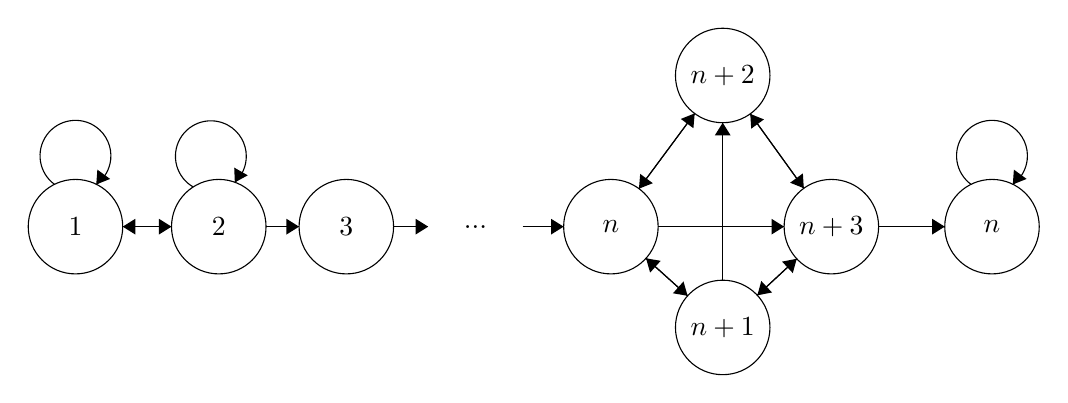
\begin{tikzpicture}[scale=0.2] \tikzstyle{every node}+=[inner sep=0pt] \draw [black] (5.5,-30.4) circle (3); \draw (5.5,-30.4) node {$1$}; \draw [black] (14.6,-30.4) circle (3); \draw (14.6,-30.4) node {$2$}; \draw [black] (22.7,-30.4) circle (3); \draw (22.7,-30.4) node {$3$}; \draw [black] (39.5,-30.4) circle (3); \draw (39.5,-30.4) node {$n$}; \draw [black] (46.6,-20.8) circle (3); \draw (46.6,-20.8) node {$n+2$}; \draw [black] (46.6,-36.8) circle (3); \draw (46.6,-36.8) node {$n+1$};
\draw (30.9,-30.4) node {$...$}; \draw [black] (53.5,-30.4) circle (3); \draw (53.5,-30.4) node {$n+3$}; \draw [black] (63.7,-30.4) circle (3); \draw (63.7,-30.4) node {$n$}; \draw [black] (8.5,-30.4) -- (11.6,-30.4); \fill [black] (11.6,-30.4) -- (10.8,-29.9) -- (10.8,-30.9); \draw [black] (17.6,-30.4) -- (19.7,-30.4); \fill [black] (19.7,-30.4) -- (18.9,-29.9) -- (18.9,-30.9); \draw [black] (41.28,-27.99) -- (44.82,-23.21); \fill [black] (44.82,-23.21) -- (43.94,-23.56) -- (44.74,-24.15); \draw [black] (41.73,-32.41) -- (44.37,-34.79); \fill [black] (44.37,-34.79) -- (44.11,-33.88) -- (43.44,-34.63); \draw [black] (46.6,-33.8) -- (46.6,-23.8); \fill [black] (46.6,-23.8) -- (46.1,-24.6) -- (47.1,-24.6); \draw [black] (25.7,-30.4) -- (27.9,-30.4); \fill [black] (27.9,-30.4) -- (27.1,-29.9) -- (27.1,-30.9); \draw [black] (33.9,-30.4) -- (36.5,-30.4); \fill [black] (36.5,-30.4) -- (35.7,-29.9) -- (35.7,-30.9); \draw [black] (4.177,-27.72) arc (234:-54:2.25); \fill [black] (6.82,-27.72) -- (7.7,-27.37) -- (6.89,-26.78); \draw [black] (12.987,-27.885) arc (240.4087:-47.5913:2.25); \fill [black] (15.62,-27.59) -- (16.44,-27.14) -- (15.58,-26.65); \draw [black] (11.6,-30.4) -- (8.5,-30.4); \fill [black] (8.5,-30.4) -- (9.3,-30.9) -- (9.3,-29.9); \draw [black] (42.5,-30.4) -- (50.5,-30.4); \fill [black] (50.5,-30.4) -- (49.7,-29.9) -- (49.7,-30.9); \draw [black] (56.5,-30.4) -- (60.7,-30.4); \fill [black] (60.7,-30.4) -- (59.9,-29.9) -- (59.9,-30.9); \draw [black] (62.377,-27.72) arc (234:-54:2.25); \fill [black] (65.02,-27.72) -- (65.9,-27.37) -- (65.09,-26.78); \draw [black] (48.8,-34.76) -- (51.3,-32.44); \fill [black] (51.3,-32.44) -- (50.37,-32.62) -- (51.05,-33.35); \draw [black] (51.75,-27.96) -- (48.35,-23.24); \fill [black] (48.35,-23.24) -- (48.41,-24.18) -- (49.22,-23.59); \draw [black] (48.35,-23.24) -- (51.75,-27.96); \fill [black] (51.75,-27.96) -- (51.69,-27.02) -- (50.88,-27.61); \draw [black] (51.3,-32.44) -- (48.8,-34.76); \fill [black] (48.8,-34.76) -- (49.73,-34.58) -- (49.05,-33.85); \draw [black] (44.37,-34.79) -- (41.73,-32.41); \fill [black] (41.73,-32.41) -- (41.99,-33.32) -- (42.66,-32.57); \draw [black] (44.82,-23.21) -- (41.28,-27.99); \fill [black] (41.28,-27.99) -- (42.16,-27.64) -- (41.36,-27.05); \end{tikzpicture} \end{center}

L'idea di questo punto 4 è ``sciogliere'' questi grovigli.

Sia $M_{3}=(S,R,V)$, introduciamo una relazione $\approx\subseteq S\times S$

$\alpha\approx\beta$ se e solo se: $(\alpha R\beta)\ e\ (\beta R\alpha)\ oppure\ \alpha=\beta$

$\approx$è una relazione di equivalenza infatti:

è riflessiva per costruzione 

è simmetrica infatti: $\alpha\approx\beta$ $(\alpha\neq\beta)$se
e solo se: $(\alpha R\beta)\ e\ (\beta R\alpha)$ se e solo se $\beta\approx\alpha$

è transitiva infatti: $\alpha\approx\beta$, \foreignlanguage{english}{$\beta\approx\gamma$
}se e solo se: $(\alpha R\beta)\ e\ (\beta R\alpha)$ e $(\gamma R\beta)\ e\ (\beta R\gamma)$,
per la transitività di $R$ si ha anche $(\alpha R\gamma),\ (\gamma R\alpha)$
da cui: $\alpha\approx\gamma$

Per questi motivi $\approx$è una relazione d'equivalenza, e come
tale partiziona l'insieme $S$ e ne definisce un insieme quoziente
$S/\approx$

Chiamiamo R-cluster la classe di equivalenza$C_{\alpha}$ di $\alpha$,
e definiamo in modo abbastanza naturale la relazione di $\leq$nel
modo seguente:

$C_{\alpha}\leq C_{\beta}$ se e solo se: $\alpha R\beta$ oppure
$C_{\alpha}=C_{\beta}$

$C_{\alpha}<C_{\beta}$ se e solo se: $\alpha R\beta$ e $C_{\alpha}\neq C_{\beta}$ 

\begin{center} 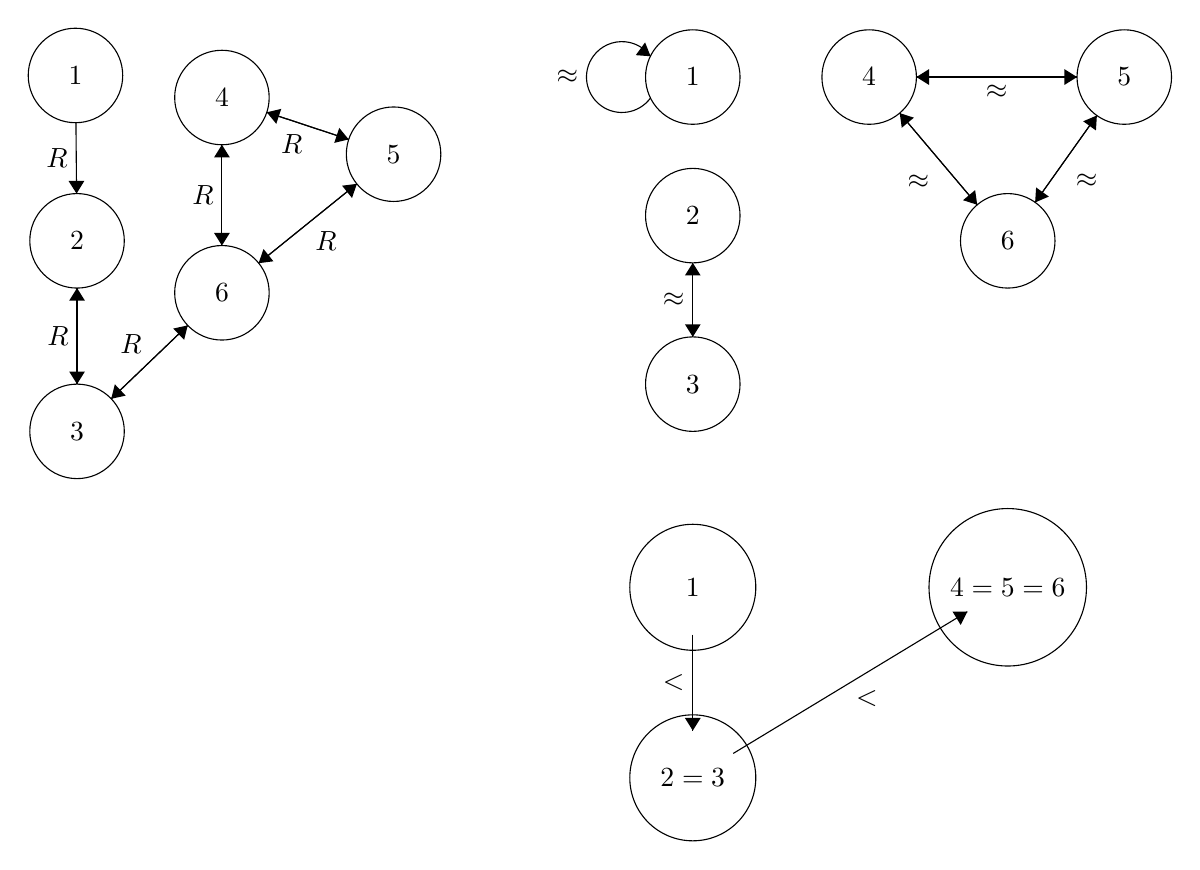
\begin{tikzpicture}[scale=0.2] \tikzstyle{every node}+=[inner sep=0pt] \draw [black] (5.1,-5.6) circle (3); \draw (5.1,-5.6) node {$1$}; \draw [black] (5.2,-16.1) circle (3); \draw (5.2,-16.1) node {$2$}; \draw [black] (5.2,-28.2) circle (3); \draw (5.2,-28.2) node {$3$}; \draw [black] (14.4,-7) circle (3); \draw (14.4,-7) node {$4$}; \draw [black] (25.3,-10.6) circle (3); \draw (25.3,-10.6) node {$5$}; \draw [black] (14.4,-19.4) circle (3); \draw (14.4,-19.4) node {$6$}; \draw [black] (44.3,-5.7) circle (3); \draw (44.3,-5.7) node {$1$}; \draw [black] (44.3,-14.5) circle (3); \draw (44.3,-14.5) node {$2$}; \draw [black] (44.3,-25.2) circle (3); \draw (44.3,-25.2) node {$3$}; \draw [black] (55.5,-5.7) circle (3); \draw (55.5,-5.7) node {$4$}; \draw [black] (71.7,-5.7) circle (3); \draw (71.7,-5.7) node {$5$}; \draw [black] (64.3,-16.1) circle (3); \draw (64.3,-16.1) node {$6$}; \draw [black] (44.3,-38.1) circle (4); \draw (44.3,-38.1) node {$1$}; \draw [black] (44.3,-50.2) circle (4); \draw (44.3,-50.2) node {$2=3$}; \draw [black] (64.3,-38.1) circle (5); \draw (64.3,-38.1) node {$4=5=6$}; \draw [black] (5.13,-8.6) -- (5.17,-13.1); \fill [black] (5.17,-13.1) -- (5.66,-12.3) -- (4.66,-12.3); \draw (4.64,-10.85) node [left] {$R$}; \draw [black] (5.2,-19.1) -- (5.2,-25.2); \fill [black] (5.2,-25.2) -- (5.7,-24.4) -- (4.7,-24.4); \draw (4.7,-22.15) node [left] {$R$}; \draw [black] (5.2,-25.2) -- (5.2,-19.1); \fill [black] (5.2,-19.1) -- (4.7,-19.9) -- (5.7,-19.9); \draw [black] (7.37,-26.13) -- (12.23,-21.47); \fill [black] (12.23,-21.47) -- (11.31,-21.67) -- (12,-22.39); \draw [black] (14.4,-10) -- (14.4,-16.4); \fill [black] (14.4,-16.4) -- (14.9,-15.6) -- (13.9,-15.6); \draw (13.9,-13.2) node [left] {$R$}; \draw [black] (14.4,-16.4) -- (14.4,-10); \fill [black] (14.4,-10) -- (13.9,-10.8) -- (14.9,-10.8); \draw [black] (17.25,-7.94) -- (22.45,-9.66); \fill [black] (22.45,-9.66) -- (21.85,-8.93) -- (21.53,-9.88); \draw (18.83,-9.34) node [below] {$R$}; \draw [black] (22.45,-9.66) -- (17.25,-7.94); \fill [black] (17.25,-7.94) -- (17.85,-8.67) -- (18.17,-7.72); \draw [black] (22.97,-12.48) -- (16.73,-17.52); \fill [black] (16.73,-17.52) -- (17.67,-17.4) -- (17.04,-16.62); \draw [black] (16.73,-17.52) -- (22.97,-12.48); \fill [black] (22.97,-12.48) -- (22.03,-12.6) -- (22.66,-13.38); \draw (21.01,-15.49) node [below] {$R$}; \draw [black] (12.23,-21.47) -- (7.37,-26.13); \fill [black] (7.37,-26.13) -- (8.29,-25.93) -- (7.6,-25.21); \draw (8.63,-23.32) node [above] {$R$}; \draw [black] (44.3,-17.5) -- (44.3,-22.2); \fill [black] (44.3,-22.2) -- (44.8,-21.4) -- (43.8,-21.4); \draw (43.8,-19.85) node [left] {$\approx$}; \draw [black] (44.3,-22.2) -- (44.3,-17.5); \fill [black] (44.3,-17.5) -- (43.8,-18.3) -- (44.8,-18.3); \draw [black] (58.5,-5.7) -- (68.7,-5.7); \fill [black] (68.7,-5.7) -- (67.9,-5.2) -- (67.9,-6.2); \draw (63.6,-6.2) node [below] {$\approx$}; \draw [black] (68.7,-5.7) -- (58.5,-5.7); \fill [black] (58.5,-5.7) -- (59.3,-6.2) -- (59.3,-5.2); \draw [black] (57.44,-7.99) -- (62.36,-13.81); \fill [black] (62.36,-13.81) -- (62.23,-12.88) -- (61.46,-13.52); \draw (59.35,-12.34) node [left] {$\approx$}; \draw [black] (66.04,-13.66) -- (69.96,-8.14); \fill [black] (69.96,-8.14) -- (69.09,-8.51) -- (69.9,-9.09); \draw (68.59,-12.27) node [right] {$\approx$}; \draw [black] (69.96,-8.14) -- (66.04,-13.66); \fill [black] (66.04,-13.66) -- (66.91,-13.29) -- (66.1,-12.71); \draw [black] (62.36,-13.81) -- (57.44,-7.99); \fill [black] (57.44,-7.99) -- (57.57,-8.92) -- (58.34,-8.28); \draw [black] (41.62,-7.023) arc (-36:-324:2.25); \draw (37.05,-5.7) node [left] {$\approx$}; \fill [black] (41.62,-4.38) -- (41.27,-3.5) -- (40.68,-4.31); \draw [black] (44.3,-41.1) -- (44.3,-47.2); 
\fill [black] (44.3,-47.2) -- (44.8,-46.4) -- (43.8,-46.4); \draw (43.8,-44.15) node [left] {$<$}; \draw [black] (46.87,-48.65) -- (61.73,-39.65); \fill [black] (61.73,-39.65) -- (60.79,-39.64) -- (61.31,-40.49); \draw (55.35,-44.65) node [below] {$<$};
\end{tikzpicture} \end{center}

Se un R-cluster C contiene più di un elemento, la relazione R è riflessiva
su $C$ e si ha $C\leq C$, infatti detti $\alpha$ e $\beta$ due
elementi di $C$ si ha $\alpha R\beta$ e $\beta R\alpha$ quindi,
per la transitività di $R$ $\alpha R\alpha$,

inoltre $C=$$C_{\alpha}\leq C\alpha$ $=C$.

Se non è $C\leq C$, l’R-cluster $C$ si dice degenere ed è formato
da un unico elemento $\alpha$ per il quale non risulta $\alpha R\alpha$ 

Un palloncino può essere visto come una sequenza finita di cluster
di cui solo l’ultimo è non degenere. Ma nel nostro modello possono
esserci, oltre all’ultimo R-cluster $C_{\alpha}$, altri R-cluster
non degeneri.

Per ricondurmi a un palloncino, a partire da $M_{3}$ considero la
relazione $R'$ che ordina in modo arbitrario i mondi appartenenti
a uno stesso R-cluster che non sia l'ultimo.

$R'$ è così definita:
\begin{itemize}
\item Se$\alpha,\beta$ appartengono a cluster diversi allora $(\alpha,\beta)\in R'$se
e solo se $(\alpha,\beta)\in R$
\item Se $\alpha,\beta$ appartengono all'ultimo cluster $(\alpha,\beta)\in R'$
\item Se $\alpha,\beta$ appartengono allo stesso cluster, e non è l'ultimo,
detti $\gamma_{1},\gamma_{2},\dots,\gamma_{n}$, si pone $\gamma_{i}R'\gamma_{j}$
se e solo se $i<j$.
\item $(\alpha,\alpha)\notin R'$ (tolgo gli autoanelli)
\end{itemize}
A questo punto abbiamo un palloncino$P$ costruito su $S$,$R'$,
$V$, ed è lecito chidersi se $\vera{M_{3}}a$ se e solo se $\vera Pa$.

Questo è ovviamente vero se $a$ non presenta connettivi modali.

Supponiamo allora che $a$ sia del tipo $\boxx d$.

Dato che$R'\subseteq R$,\\
\begin{center} 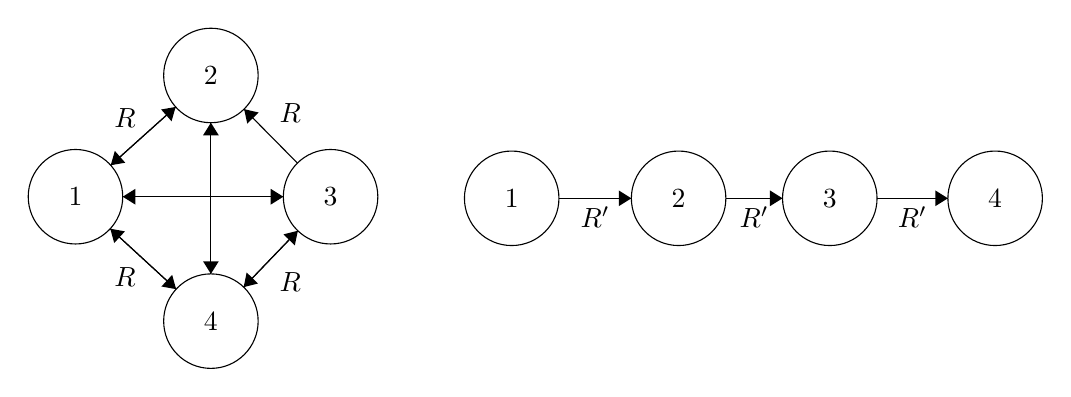
\begin{tikzpicture}[scale=0.2] \tikzstyle{every node}+=[inner sep=0pt] \draw [black] (11,-13.3) circle (3); \draw (11,-13.3) node {$1$}; \draw [black] (19.6,-5.6) circle (3); \draw (19.6,-5.6) node {$2$}; \draw [black] (27.2,-13.3) circle (3); \draw (27.2,-13.3) node {$3$}; \draw [black] (19.6,-21.2) circle (3); \draw (19.6,-21.2) node {$4$}; \draw [black] (38.7,-13.4) circle (3); \draw (38.7,-13.4) node {$1$}; \draw [black] (49.3,-13.4) circle (3); \draw (49.3,-13.4) node {$2$}; \draw [black] (58.9,-13.4) circle (3); \draw (58.9,-13.4) node {$3$}; \draw [black] (69.4,-13.4) circle (3); \draw (69.4,-13.4) node {$4$}; \draw [black] (13.24,-11.3) -- (17.36,-7.6); \fill [black] (17.36,-7.6) -- (16.44,-7.76) -- (17.1,-8.51); \draw [black] (17.36,-7.6) -- (13.24,-11.3); \fill [black] (13.24,-11.3) -- (14.16,-11.14) -- (13.5,-10.39); \draw (14.14,-8.96) node [above] {$R$}; \draw [black] (25.09,-11.16) -- (21.71,-7.74); \fill [black] (21.71,-7.74) -- (21.91,-8.66) -- (22.63,-7.95); \draw (23.93,-7.98) node [right] {$R$}; \draw [black] (17.39,-19.17) -- (13.21,-15.33); \fill [black] (13.21,-15.33) -- (13.46,-16.24) -- (14.14,-15.5); \draw (14.14,-17.74) node [below] {$R$}; \draw [black] (13.21,-15.33) -- (17.39,-19.17); \fill [black] (17.39,-19.17) -- (17.14,-18.26) -- (16.46,-19); \draw [black] (21.68,-19.04) -- (25.12,-15.46); \fill [black] (25.12,-15.46) -- (24.21,-15.69) -- (24.93,-16.39); \draw (23.93,-18.72) node [right] {$R$}; \draw [black] (25.12,-15.46) -- (21.68,-19.04); \fill [black] (21.68,-19.04) -- (22.59,-18.81) -- (21.87,-18.11); \draw [black] (19.6,-8.6) -- (19.6,-18.2); \fill [black] (19.6,-18.2) -- (20.1,-17.4) -- (19.1,-17.4); \draw [black] (19.6,-18.2) -- (19.6,-8.6); \fill [black] (19.6,-8.6) -- (19.1,-9.4) -- (20.1,-9.4); \draw [black] (24.2,-13.3) -- (14,-13.3); \fill [black] (14,-13.3) -- (14.8,-13.8) -- (14.8,-12.8); \draw [black] (14,-13.3) -- (24.2,-13.3); \fill [black] (24.2,-13.3) -- (23.4,-12.8) -- (23.4,-13.8); \draw [black] (41.7,-13.4) -- (46.3,-13.4); \fill [black] (46.3,-13.4) -- (45.5,-12.9) -- (45.5,-13.9); \draw (44,-13.9) node [below] {$R'$}; \draw [black] (52.3,-13.4) -- (55.9,-13.4); \fill [black] (55.9,-13.4) -- (55.1,-12.9) -- (55.1,-13.9); \draw (54.1,-13.9) node [below] {$R'$}; \draw [black] (61.9,-13.4) -- (66.4,-13.4); \fill [black] (66.4,-13.4) -- (65.6,-12.9) -- (65.6,-13.9); \draw (64.15,-13.9) node [below] {$R'$}; \end{tikzpicture} \end{center} 

se $\boxx d$ è vera in un mondo $\beta$ di $M_{3}$, $\boxx d$
è vera anche nel mondo $\beta$ di $M\lyxmathsym{’}$ ($R'$ ha
meno archi quindi è più facile per $\boxx x$ essere soddisfatta)

Sia allora $\boxx d$ vera in un mondo $\beta$ di $M\lyxmathsym{’}$
e supponiamo che $\boxx d$ non sia vera nel mondo $\beta$ di $M_{3}$.

Se è così, $d$ dovrà allora risultare falsa in un mondo $\gamma$
tale che $(\beta,\gamma)\in R$ mentre $(\beta,\gamma)\notin R\lyxmathsym{’}$.

\begin{center} 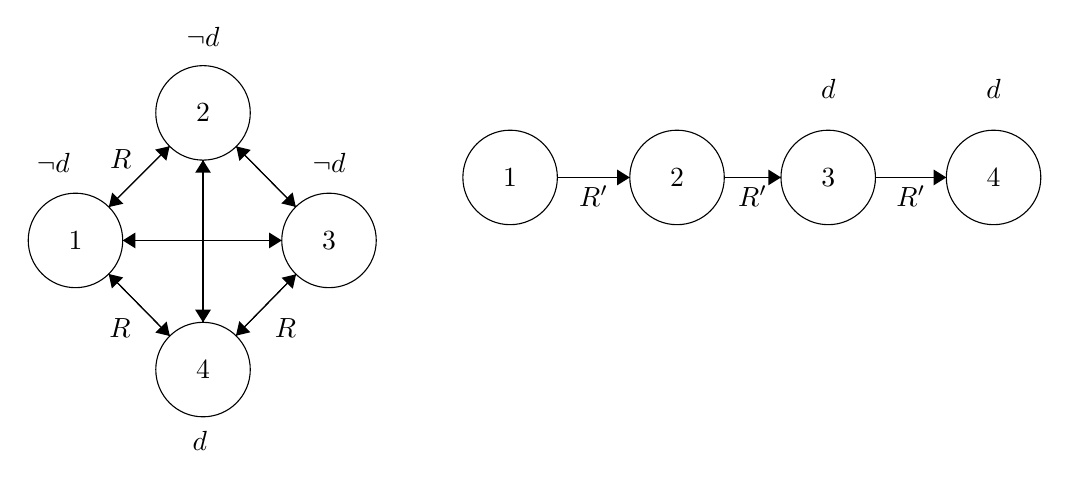
\begin{tikzpicture}[scale=0.2] \tikzstyle{every node}+=[inner sep=0pt] \draw [black] (11.1,-17.4) circle (3); \draw (11.1,-17.4) node {$1$}; \draw [black] (19.2,-9.3) circle (3); \draw (19.2,-9.3) node {$2$}; \draw [black] (27.2,-17.4) circle (3); \draw (27.2,-17.4) node {$3$}; \draw [black] (19.2,-25.6) circle (3); \draw (19.2,-25.6) node {$4$}; \draw [black] (38.7,-13.4) circle (3); \draw (38.7,-13.4) node {$1$}; \draw [black] (49.3,-13.4) circle (3); \draw (49.3,-13.4) node {$2$}; \draw [black] (58.9,-13.4) circle (3); \draw (58.9,-13.4) node {$3$}; \draw [black] (69.4,-13.4) circle (3); \draw (69.4,-13.4) node {$4$};
\draw (27.2,-12.5) node {$\neg\boxx d$};
\draw (19.2,-4.5) node {$\neg d$};
\draw (9.7,-12.5) node {$\neg d$};
\draw (19,-30.1) node {$d$};
\draw (58.9,-7.8) node {$\boxx d$};
\draw (69.4,-7.8) node {$d$}; 
\draw [black] (13.22,-15.28) -- (17.08,-11.42); 
\fill [black] (17.08,-11.42) -- (16.16,-11.63) -- (16.87,-12.34); \draw [black] (17.08,-11.42) -- (13.22,-15.28); 
\fill [black] (13.22,-15.28) -- (14.14,-15.07) -- (13.43,-14.36); \draw (13.98,-12.87) node [above] {$R$}; 
\draw [black] (25.09,-15.27) -- (21.31,-11.43); \fill [black] (21.31,-11.43) -- (21.51,-12.35) -- (22.23,-11.65);
\draw [black] (17.09,-23.47) -- (13.21,-19.53); \fill [black] (13.21,-19.53) -- (13.41,-20.45) -- (14.13,-19.75); 
\draw (14.63,-22.97) node [left] {$R$}; \draw [black] (13.21,-19.53) -- (17.09,-23.47); \fill [black] (17.09,-23.47) -- (16.89,-22.55) -- (16.17,-23.25); \draw [black] (21.29,-23.45) -- (25.11,-19.55); \fill [black] (25.11,-19.55) -- (24.19,-19.77) -- (24.9,-20.47); 
\draw (23.73,-22.97) node [right] {$R$}; \draw [black] (25.11,-19.55) -- (21.29,-23.45); \fill [black] (21.29,-23.45) -- (22.21,-23.23) -- (21.5,-22.53); \draw [black] (19.2,-12.3) -- (19.2,-22.6); \fill [black] (19.2,-22.6) -- (19.7,-21.8) -- (18.7,-21.8); \draw [black] (19.2,-22.6) -- (19.2,-12.3); \fill [black] (19.2,-12.3) -- (18.7,-13.1) -- (19.7,-13.1); \draw [black] (24.2,-17.4) -- (14.1,-17.4); \fill [black] (14.1,-17.4) -- (14.9,-17.9) -- (14.9,-16.9); \draw [black] (14.1,-17.4) -- (24.2,-17.4); \fill [black] (24.2,-17.4) -- (23.4,-16.9) -- (23.4,-17.9); \draw [black] (41.7,-13.4) -- (46.3,-13.4); \fill [black] (46.3,-13.4) -- (45.5,-12.9) -- (45.5,-13.9); \draw (44,-13.9) node [below] {$R'$}; \draw [black] (52.3,-13.4) -- (55.9,-13.4); \fill [black] (55.9,-13.4) -- (55.1,-12.9) -- (55.1,-13.9); \draw (54.1,-13.9) node [below] {$R'$}; \draw [black] (61.9,-13.4) -- (66.4,-13.4); \fill [black] (66.4,-13.4) -- (65.6,-12.9) -- (65.6,-13.9); \draw (64.15,-13.9) node [below] {$R'$}; \draw [black] (21.31,-11.43) -- (25.09,-15.27); \fill [black] (25.09,-15.27) -- (24.89,-14.35) -- (24.17,-15.05); \end{tikzpicture} \end{center} 

Ovviamente se $(\beta,\gamma)\in R$ ma $(\beta,\gamma)\notin R\lyxmathsym{’}$,
i mondi $\beta,\gamma$ devono appartenere ad uno stesso R- cluster
che non è l’ultimo. (infatti se $(\beta,\gamma)\in R$ allora sono
nello stesso cluster, che viene ``sciolto'' in R')

Si può ora far uso dello Z-lemma che garantisce l’esistenza di un
mondo $\delta$ in un R- cluster $C_{\delta}$ tale che $C_{\beta}<C_{\delta}$
in cui $d$ non è vera (lo Z-lemma sarà enunciato e dimostrato nel
seguito).

Ma $C_{\beta}<C_{\delta}$ implica $(\beta,\delta)\in R\lyxmathsym{’}$
e dunque $\boxx d$ non sarebbe vera nel mondo $\beta$ del modello
M’, contro la nostra supposizione.

Dunque avendo dimostrato nel passo 3 che $a$ non è vera nel mondo
$\alpha$ del modello $M_{3}$, abbiamo che $a$ non è vera nel mondo
$\alpha$ del modello $M\lyxmathsym{’}$, costruito su un palloncino
e quindi $a$ non è valida su ogni palloncino.

\textbf{5) }Esiste un p-morfismo suriettivo da $(\omega,<)$ a un
palloncino P.

Sia P : $(T,\rho)$ dove 

$T=\{\alpha_{1},\alpha_{2},...,\alpha_{n},\alpha_{n+1},...,\alpha_{n+m}\}$
e 

$i.j\in\rho\ \iff\ i<j\ oppure\ i,j\geq n$ 

L'idea è di fare un p-morfismo la cui funzione f : manda i primi $n$
mondi di $\omega$ nel ``gambo'' e i mondi da $n+1$ in poi nella
parte ``tonda'' del palloncino contando modulo $m$.

Pertando definiamo $f\ :\ \omega\rightarrow T$ (ricordando che i
mondi sono numerati, sia in $\omega$ che in $T$)

$f(i)=i\ se$$i\leq m+n$

$f(n+m+j)=n+((m+j)\ mod\ 4)$

$f$ è suriettiva (tutto il codominio $T$ è raggiunto)

Infatti ogni elemento $i\in T$ ha almeno controimmagine $i\in\omega$
(gli elementi nella parte ``tonda'' del palloncino ne avranno altre)

\framebox{\begin{minipage}[t]{1\columnwidth}%
Proprietà di un p-morfismo

1) $(\alpha,\,\beta)\in R_{1}\implies(f(\alpha),\, f(\beta))\in R_{2}$

2) $(f(\alpha),\,\eta)\in R_{2}\implies\exists\beta\in S_{1}\,:\, f(\beta)=\eta\,\wedge\,(\alpha,\,\beta)\in R_{1}$%
\end{minipage}}

1) Se $\alpha,\beta<n$ si ha banalmente $f(\alpha),f(\beta)$ per
come è definita $f$ ;

Se$f(\alpha),f(\beta)$ sono nella parte ``tonda'' la 1) vale perché
$f(\alpha),f(\beta)$ in relazione di equivalenza

Se $\alpha$ nel gambo e $\beta$ nella parte ``tonda'', comunque
vale la 1) ricordando la transitività di $\rho$

2) Se $f(\alpha)<\eta$ basta prendere come $\beta$ proprio$\eta$
da $\omega$ e quindi avere $\alpha<\eta$

Se $f(\alpha)>\eta$ posso comunque trovare \textbf{$\beta$ }opportuno
sfruttando l'aritmetica modulare.



Quindi se $a$ non è valida su ogni palloncino non è valida su $(\omega,<)$,
contro l’ipotesi, pertanto $a$ deve essere un teorema di $\Omega$.


\section{Z-Lemma}

preso un modello $\mu$ finito, seriale, transitivo, connesso, su
cui è vero l'assioma Z, se la formula $\boxx b$ è falsa in un mondo
$\alpha$ che non appartenga all'ultimo R-cluster allora esiste in
$\beta$ in un cluster successivo $c_{\alpha}$ in cui b è falso.

Ip) $\mu$ finito, seriale, transitivo, connesso e vale Z. In un cluster
$C_{\alpha}$ esiste un mondo $\alpha$ in cui non vale $\boxx b$

Ts) $\nonveraw{\mu}{\beta}b$ per tutti i $\beta$ appartenenti a
r-cluster successivi a $C_{\alpha}$

Per assurdo, supponiamo:

$\veraw{\mu}{\beta}b$ per ogni $\beta$ appartenente ai cluster successivi
a $C_{\alpha}$

allora deve valere

$\nonveraw{\mu}{\delta}b$ in qualche mondo $\delta$ tale che $C_{\alpha}=C_{\delta}$

\begin{center}  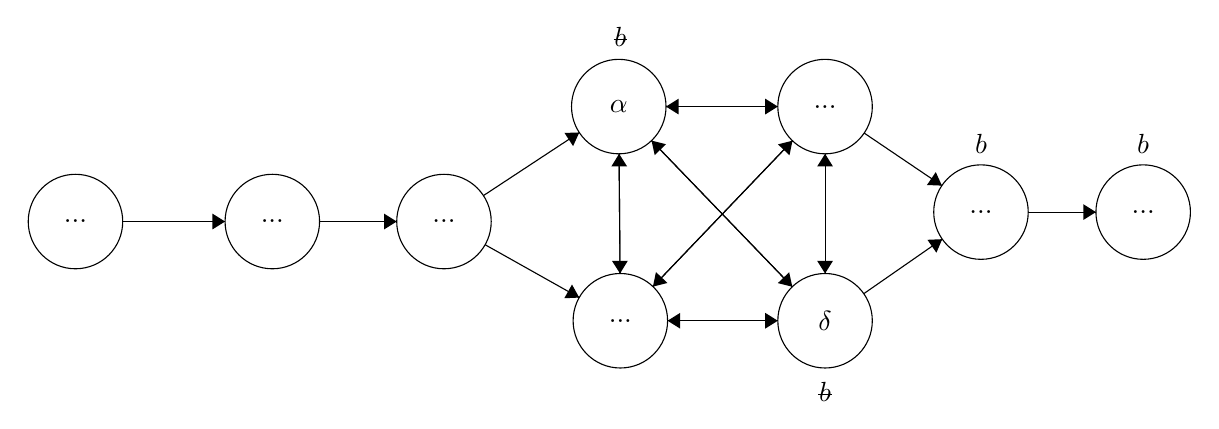
\begin{tikzpicture}[scale=0.2]  \tikzstyle{every node}+=[inner sep=0pt]  \draw [black] (6.9,-25) circle (3);  \draw (6.9,-25) node {$...$};  \draw [black] (19.4,-25) circle (3);  \draw (19.4,-25) node {$...$};  \draw [black] (30.3,-25) circle (3);  \draw (30.3,-25) node {$...$};  \draw [black] (41.4,-17.7) circle (3);  \draw (41.4,-17.7) node {$\alpha$};  \draw [black] (41.5,-31.3) circle (3);  \draw (41.5,-31.3) node {$...$};  \draw [black] (54.5,-17.7) circle (3); \draw (54.5,-17.7) node {$...$}; \draw [black] (54.5,-31.3) circle (3);  \draw (54.5,-31.3) node {$\delta$};  \draw [black] (64.4,-24.4) circle (3);  \draw (64.4,-24.4) node {$...$};  \draw [black] (74.7,-24.4) circle (3);  \draw (74.7,-24.4) node {$...$};  \draw (74.7,-20.1) node {$b$};  \draw (64.4,-20.1) node {$b$};  \draw (54.5,-35.8) node {\sout{$b$}};  \draw (41.5,-13.3) node {\sout{$\boxx{b}$}};  \draw [black] (9.9,-25) -- (16.4,-25);  \fill [black] (16.4,-25) -- (15.6,-24.5) -- (15.6,-25.5);  \draw [black] (22.4,-25) -- (27.3,-25);  \fill [black] (27.3,-25) -- (26.5,-24.5) -- (26.5,-25.5);  \draw [black] (32.81,-23.35) -- (38.89,-19.35);  \fill [black] (38.89,-19.35) -- (37.95,-19.37) -- (38.5,-20.21);  \draw [black] (32.91,-26.47) -- (38.89,-29.83);  \fill [black] (38.89,-29.83) -- (38.43,-29) -- (37.94,-29.87);  \draw [black] (41.48,-28.3) -- (41.42,-20.7);  \fill [black] (41.42,-20.7) -- (40.93,-21.5) -- (41.93,-21.5);  \draw [black] (41.42,-20.7) -- (41.48,-28.3);  \fill [black] (41.48,-28.3) -- (41.97,-27.5) -- (40.97,-27.5);  \draw [black] (51.5,-31.3) -- (44.5,-31.3);  \fill [black] (44.5,-31.3) -- (45.3,-31.8) -- (45.3,-30.8);  \draw [black] (44.5,-31.3) -- (51.5,-31.3);  \fill [black] (51.5,-31.3) -- (50.7,-30.8) -- (50.7,-31.8);  \draw [black] (54.5,-28.3) -- (54.5,-20.7); \fill [black] (54.5,-20.7) -- (54,-21.5) -- (55,-21.5); \draw [black] (54.5,-20.7) -- (54.5,-28.3); \fill [black] (54.5,-28.3) -- (55,-27.5) -- (54,-27.5);  \draw [black] (51.5,-17.7) -- (44.4,-17.7); \fill [black] (44.4,-17.7) -- (45.2,-18.2) -- (45.2,-17.2); \draw [black] (44.4,-17.7) -- (51.5,-17.7); \fill [black] (51.5,-17.7) -- (50.7,-17.2) -- (50.7,-18.2); \draw [black] (52.43,-19.87) -- (43.57,-29.13); \fill [black] (43.57,-29.13) -- (44.49,-28.9) -- (43.76,-28.21); \draw [black] (43.57,-29.13) -- (52.43,-19.87); \fill [black] (52.43,-19.87) -- (51.51,-20.1) -- (52.24,-20.79); \draw [black] (43.48,-19.86) -- (52.42,-29.14);  \fill [black] (52.42,-29.14) -- (52.22,-28.22) -- (51.5,-28.91);  \draw [black] (52.42,-29.14) -- (43.48,-19.86); \fill [black] (43.48,-19.86) -- (43.68,-20.78) -- (44.4,-20.09);  \draw [black] (56.96,-29.58) -- (61.94,-26.12);  \fill [black] (61.94,-26.12) -- (61,-26.16) -- (61.57,-26.98);  \draw [black] (56.98,-19.38) -- (61.92,-22.72); \fill [black] (61.92,-22.72) -- (61.53,-21.86) -- (60.97,-22.68); \draw [black] (67.4,-24.4) -- (71.7,-24.4);  \fill [black] (71.7,-24.4) -- (70.9,-23.9) -- (70.9,-24.9);  \end{tikzpicture}  \end{center}

allora, poichè la trelazione è transitiva e connessa, abbiamo che

$\nonveraw{\mu}{\gamma}{\boxx b}$

e quindi, per questo possiamo dire che vale:

$\veraw{\mu}{\gamma}{\boxx b\implies b}$

per ogni cluster precedente a $C_{\alpha}$ e a $C_{\alpha}$stesso,
essendo falso il suo antecedente.

ma poichè in tutti i mondi successivi è vera b, allora in tutti i
mondi del modello è vera:

$\vera{\mu}{\boxx{(\boxx{b\implies b)}}}$

Però applicando a questo punto il modus ponens all'assioma Z e alla
precedente abbiamo che vale:

$\vera{\mu}{\diam{\boxx b}\implies\boxx b}$

Poichè per tutti i mondi dopo $C_{\alpha}$ è vera b, allora è vera
anche $\boxx b$

Ma allora in $\alpha$ vale:

$\veraw{\mu}{\alpha}{\diam{\boxx b}}$ 

poichè esistono dei mondi raggiungibili in cui è vera $\boxx b$

ma allora per Modus Ponens, è vale anche:

$\veraw{\mu}{\alpha}{\boxx b}$

Assurdo! La tesi allora deve essere valida.


\section{Altre logiche temporali}

Ci sono altre due logiche temporali interessanti:
\begin{enumerate}
\item K4DLDum, corretta e completa sul frame ($\omega$, $\leq$)
\item K4DLX corretta e completa sui frame ($\mathbb{Q}$,<) e ($\mathbb{R}$,<)
\end{enumerate}
Dove all'assioma Z vengono sostituiti rispettivamente:
\begin{itemize}
\item Dum: $\boxx{(\boa\implies a)\implies(\diam{\boa}\implies\boa)}$
\item X: $\boxx{\boa}\implies\boa$
\end{itemize}
Come si può notare non si può distinguere un tempo numerabile da un
tempo continuo.



\chapter{Logica Multimodale - Back To The Future}


\section{Logiche multimodali}

una logica multimodale è una logica che definisce oltre ai normali
operatori della logica proposizionale gli operatori:

$[i]$ con $i\in I$

$<i>\equiv\neg[i]\neg$

definita sul frame:

$F=(S,\{R_{i}\,|\, i\in I\})$ 

La semantica di una logica multimodale è la stessa della logica proposizionale
per gli operatori comuni, mentre gli operatori box hanno la seguente
semantica:

$\veraw{\mu}{\alpha}{\neci ia}\iff\veraw{\mu}{\beta}a\,\forall\beta\,:\,(\alpha,\,\beta)\in R_{i}$

Chiamiamo assioma $K_{i}$ la seguente formula:

$K_{i}$: $\neci i{(a\implies b)}\implies(\neci ia\implies\neci i{b)}$

Tutte le logiche multimodali normali devono contenere:

gli assiomi $K_{i}$ $\forall i\in I$

le regole di necessitazione:

$RN_{i}:$ $\dfrac{a}{\neci ia}$ $\forall i\in I$


\section{Futuro e Passato}

Possiamo applicare le logiche multimodali al concetto di tempo, per
farlo consideriamo il frame:

$F=(S,\,\{R_{P},\, R_{e}\})$

da cui possiamo ricavare gli operatori modali:

$[P]$ e $[F]$

ricordiamo che:

$<P>\equiv\neg[P]\neg$

$<F>\equiv\neg[F]\neg$

Perchè le due relazioni rappresentino il tempo che scorre una deve
essere l'opposta dell'altra, in modo che la prima relazione rappresenti
il futuro, la seconda il passato:

$\alpha R_{P}\beta\iff\beta R_{F}\alpha$

$R_{p}=R_{f}^{-1}$

Questa proprietà si può dimostrare equivalente ai due assiomi:

$B_{PF}:$ $a\implies\necp{\posf a}$

$B_{FP}:$ $a\implies\necf{\posp a}$


\subsection{Dimostrazione}

Ip) $\veraw{\mu}{\alpha}a$ e $\forall\beta\,:\,(\alpha,\,\beta)\in R_{P}\iff(\beta,\,\alpha)\in R_{F}$

Ts) $\veraw{\mu}{\alpha}{\necp{\posf a}}$

Ogni mondo $\beta$ raggiunge $\alpha$ tramite $R_{F}$, e quindi:

$\veraw{\mu}{\beta}{\posf a}$

allora, usando la regola di necessitazione nel passato, possiamo scrivere:

$\veraw{\mu}{\alpha}{\necp{\posf a}}$

ma poichè per ipotesi in $\alpha$ è vera a:

$\veraw{\mu}{\alpha}{\necp{\posf a}}$

poichè abbiamo preso un $\alpha$ generico, la tesi è dimostrata.\\
Ip) $\veraw{\mu}{\alpha}{\necp{\posf a}}$

Ts) $R_{F}=R_{P}$

per assurdo $R_{F}\neq R_{p}$

prendiamo allora un mondo $\alpha$ in cui a $R_{P}$ non corrisponda
l'arco inverso nella relazione $R_{F}$

$V(A)=\{\alpha\}$

allora in $\beta$ poichè non si raggiunge tramite $R_{P}$ il mondo
$\alpha$ vale:

$\nonveraw{\mu}{\beta}{\posf A}$

ma poichè $\beta$ è raggiungibile da $\alpha$ tramite $R_{P}$ abbiamo:

$\nonveraw{\mu}{\alpha}{\necp{\posf A}}$

Ma allora, poichè in $\alpha$ è vera A:

$\nonveraw{\mu}{\alpha}{A\implies\necp{\posf A}}$

Assurdo! allora la tesi è dimostrata.

\begin{center} 
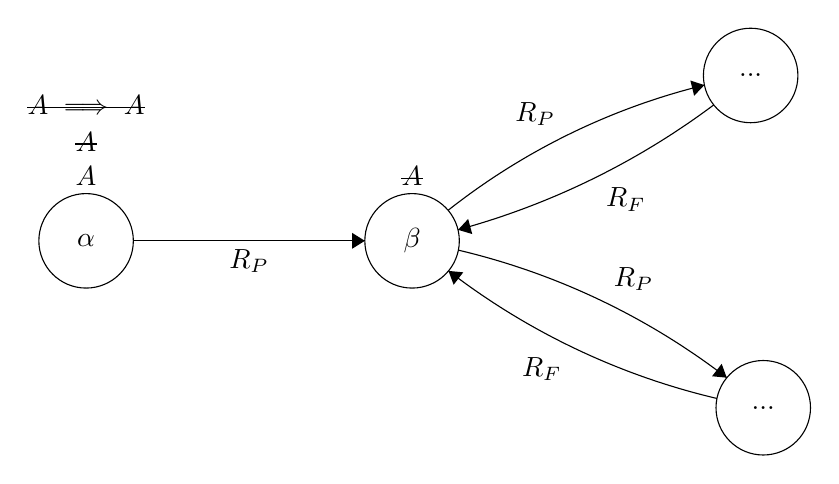
\begin{tikzpicture}[scale=0.2] 
\tikzstyle{every node}+=[inner sep=0pt] 
\draw [black] (17,-27.7) circle (3); 
\draw (17,-27.7) node {$\alpha$}; 
\draw [black] (37.7,-27.7) circle (3); 
\draw (37.7,-27.7) node {$\beta$}; 
\draw [black] (59.2,-17.2) circle (3); 
\draw (59.2,-17.2) node {$...$}; 
\draw [black] (60,-38.3) circle (3); 
\draw (60,-38.3) node {$...$}; 
\draw (17,-23.6) node {$A$}; 
\draw (37.7,-23.6) node {\sout{$\posf{A}$}}; 
\draw (17,-21.4) node {\sout{$\necp{\posf{A}}$}}; 
\draw (17,-19.1) node {\sout{$A\implies \necp{\posf{A}}$}}; 
\draw [black] (40.641,-28.292) arc (76.71074:52.44238:44.889);
\fill [black] (57.68,-36.39) -- (57.36,-35.51) -- (56.75,-36.3);
\draw (51.76,-30.92) node [above] {$R_P$}; 
\draw [black] (39.988,-25.761) arc (128.26646:103.79273:42.728);
\fill [black] (56.26,-17.81) -- (55.37,-17.52) -- (55.61,-18.49); 
\draw (45.52,-20.4) node [above] {$R_P$};
\draw [black] (20,-27.7) -- (34.7,-27.7);
\fill [black] (34.7,-27.7) -- (33.9,-27.2) -- (33.9,-28.2);
\draw (27.35,-28.2) node [below] {$R_P$}; 
\draw [black] (56.855,-19.07) arc (-53.2117:-74.72911:48.403);
\fill [black] (40.62,-27) -- (41.52,-27.27) -- (41.26,-26.31);
\draw (51.28,-24.31) node [below] {$R_F$}; 
\draw [black] (57.059,-37.71) arc (-103.2634:-127.58348:44.797); 
\fill [black] (40.01,-29.61) -- (40.34,-30.49) -- (40.95,-29.7); 
\draw (45.94,-35.08) node [below] {$R_F$}; 
\end{tikzpicture} 
\end{center}


\section{Frame Temporale}

Un frame temporale è un frame così composto:

$F=(S,\, R_{F})$

con $R_{F}=R_{p}^{-1}$ e $R_{F}$ transitiva.

In un frame temporale devono valere gli assiomi:

A1, A2, A3, $K_{P}$, $K_{F}$, $4_{P}$, $4_{F}$, $B_{FP}$, $B_{PF}$

dove gli assiomi che esprimono la transitività sono:

$4_{P}$: $\necf a\implies\necf{\necf a}$

$4_{F}$: $\necp a\implies\necp{\necp a}$

$B_{PF}:$ $a\implies\necp{\posf a}$

$B_{FP}:$ $a\implies\necf{\posp a}$\\


Una logica temporale è una logica normale multimodale nei connettivi
modali {[}F{]} e {[}P{]}

che contiene gli schemi $B_{FP}$ $B\mbox{\ensuremath{_{PF}}}$$4_{P}$
$4_{F}$.

Si dice logica lineare temporale ogni logica normale che contiene
la minima

logica normale temporale $Kt$

$Kt$ si assiomatizza con $A1,\ A2,\ A3,\ MP,\ K_{P},\ K_{F},\ B_{PF},\ B_{FP},\ 4_{P},\ 4_{F},\ RN_{P},\ RN_{F}$


\section{Correttezza, completezza e decidibilità nelle logiche multimodali}

Possiamo seguire lo stesso schema di dimostrazioni usato nella logica
unimodale per dimostrare la correttezza, completezza e decidibilità
delle logiche multimodali. Bisogna tuttavia ridefinire alcuni dettagli,
ossia il teorema di raggiungibilità e la $\Gamma$-Filtrazione


\subsection{Teorema di Raggiungibilità}

$(\alpha,\,\beta)\in R^{\Lambda}$

è equivalente a:

$\{a\,|\,\necf a\in\alpha\}\subseteq\beta$

oppure:

$\{\posf{b\,|\, b\in\beta\}\subseteq\alpha}$


\subsection{$\Gamma$-Filtrazione}

Bisogna, nel caso delle logiche multimodali, ridefinire il concetto
di relazione filtrata R'.

R' infatti dovrà ora soddisfare le tre seguenti proprietà:

F1) $(\alpha,\,\beta)\in R\implies([\alpha],\,[\beta])\in R'$

F2) $([\alpha],\,[\beta])\in R'\implies(\forall\necf b\in\Gamma\,\veraw{\mu}{\alpha}{\necf b}\implies\veraw{\mu}{\beta}b)$

F3) $([\alpha],\,[\beta])\in R'\implies(\forall\necp b\in\Gamma\,\veraw{\mu}{\beta}{\necp b}\implies\veraw{\mu}{\alpha}b)$


\section{Distinzione tra ($\mathbb{Q}$ ,<) e ($\mathbb{R}$ ,<)}

Nella logica unimodale non siamo in grado di distinguere i frame ($\mathbb{Q}$
,<) e ($\mathbb{R}$ ,<), entrambi sono espressi dalla logica K4DLX

Per convenzione poniamo:

$\boa\equiv\necp a\wedge a\wedge\necf a$

L'assioma che esprime la continuità della relazione è il seguente:

Cont: $\boxx{(\necp a\implies\posf{\necp{a)}}\implies(\necp a\implies\necf{a)}}$

Si dimostra che:

$\nonvera{(\mathbb{Q},<)}{Cont}$

$\vera{(\mathbb{R},<)}{Cont}$\\
\\
Ip) $V(A)=\{q\in\mathbb{Q}\,|\, q<\sqrt{2}\}$

Ts) $\nonvera{(\mathbb{Q},<)}{Cont}$

Preso $\alpha<\sqrt{2}$, varranno:

$\veraw{\mu}{\alpha}{\necp A}$

$\nonveraw{\mu}{\alpha}{\necf A}$

e quindi possiamo scrivere $\forall\alpha<\sqrt{2}$

$\nonveraw{\mu}{\alpha}{\necp A\implies\necf A}$

Tuttavia l'antecedente di Cont è vero, infatti $\forall\alpha<\sqrt{2}$:

$\veraw{\mu}{\alpha}{\posf{\necp A}}$ 

e quindi l'antecedente di Cont è vero

mentre $\forall\alpha>\sqrt{2}$ vale:

$\nonveraw{\mu}{\alpha}{\necp A}$

e quindi l'antecedente di Cont è ancora vero.

Poichè l'antecedente di Cont è sempre vero, mentre la conseguenza
no, allora:

$\nonvera{(\mathbb{Q},<)}{Cont}$

e la tesi è dimostrata.\\


  \definecolor{cc60000}{RGB}{198,0,0} \definecolor{c800000}{RGB}{128,0,0}
\begin{tikzpicture}[y=0.80pt,x=0.80pt,yscale=-1, 
inner sep=0pt, outer sep=0pt] \begin{scope}[shift={(0,-752.36216)}] 
 \path[shift={(0,752.36216)},draw=black,line join=miter,line 
cap=butt,line     width=0.800pt] (30.0000,55.0000) -- (578.6159,55.0000);
  \path[draw=cc60000,fill=c800000,line join=miter,line cap=butt,line    
width=1.176pt] (318.0000,789.0651) .. controls (317.7036,818.9733)
and     (318.0000,817.6504) .. (318.0000,817.6504);  
\path[shift={(0,752.36216)},fill=black] (344.70734,136.11012) node[above right]  
  (text3993) {};  
\path[fill=black] (305.92676,776.86609) 
node[above right] (text4078) {$\sqrt{2}$}; 

\path[shift={(0,752.36216)},fill=black] 
(489.36133,76.863548) node[above right]     (text4105) {};  
\path[draw=black,line join=miter,line cap=butt,line width=0.710pt]  
  (254.0000,817.9182) -- (254.0000,788.8061);   \path[fill=black]

(235.91389,777.67352) node[above right] (text4228) {$\alpha$};  

\path[cm={{0.09011,0.0,0.0,0.12041,(552.7687,781.39932)}},draw=black,fill=black]   
 (354.7100,211.5149) -- (302.2148,240.5337) -- (250.8362,271.4865) -- 
   (251.9528,211.5149) -- (250.8362,151.5433) -- (302.2148,182.4960) -- cycle;
\end{scope}
\end{tikzpicture} 

Ip) $\delta=\max\limits _{\eta\in\mathbb{R}}(\veraw{\mu}{\eta}{A\,\eta<\delta)}$

Ts) $\vera{(\mathbb{R},<)}{Cont}$

$\forall\alpha<\delta$ possiamo scrivere:

$\veraw{\mu}{\alpha}{\necp A}$

$\nonveraw{\mu}{\alpha}{\necf A}$

Tuttavia l'antecedente di Cont è falso, infatti:

$\veraw{\mu}{\delta}{\necp A}$

ma poichè non può esistere nessun mondo $\xi>\delta$ in cui sia vera
A, essendo $\delta$ massimo, avremo che:

$\nonveraw{\mu}{\delta}{\posf{\necp A}}$

e quindi non potrà che essere che:

$\veraw{\mu}{\delta}{\necp a\implies\posf{\necp a}}$

Poichè $\delta$ è raggiungibile da a avremo che:

$\veraw{\mu}{\alpha}{\boxx{(\necp a\implies\posf{\necp a})}}$

allora avremo che in $\alpha$ l'antecedente di Cont è falso solo
quando è falso il conseguente, e quindi il teorema è dimostrato.\\
\begin{tikzpicture}[y=0.80pt,x=0.80pt,yscale=-1, inner sep=0pt, outer sep=0pt] 
\begin{scope}[shift={(0,-752.36216)}]  
\path[shift={(0,752.36216)},draw=black,line join=miter,line cap=butt,line   
 width=0.800pt] (30.0000,55.0000) -- (578.6159,55.0000);  
\path[shift={(0,752.36216)},fill=black] (344.70734,136.11012) node[above right]     (text3993) {};

\path[fill=black] (360.87012,839.06793) node[above right] (text4078) {$\gamma$};  

\path[shift={(0,752.36216)},fill=black] (489.36133,76.863548) node[above right]    (text4105) {}; 
\path[draw=black,line join=miter,line cap=butt,line width=0.777pt] 
(276.0850,827.9182) -- (276.0850,799.3622);  

\path[fill=black] (210.22182,794.57617) node[above right] (text4228) {$\alpha$};

  \path[cm={{0.09011,0.0,0.0,0.12041,(552.7687,781.39932)}},draw=black,fill=black]  
  (354.7100,211.5149) -- (302.2148,240.5337) -- (250.8362,271.4865) --    
(251.9528,211.5149) -- (250.8362,151.5433) -- (302.2148,182.4960) -- cycle; 
 \path[shift={(0,752.36216)},draw=black,line join=miter,line cap=butt,line 
   width=0.800pt] (230.0000,54.5911) -- (230.0000,90.0000) -- (30.0000,90.0000);  

\path[fill=black] (263.79507,789.35651) node[above right] (text4725) {[p]a};  
\path[fill=black] (262.00568,840.79724) node[above right] (text4729) {$\delta$};  

\path[shift={(0,752.36216)},draw=black,line join=miter,line cap=butt,line    
width=0.800pt] (359.6890,47.0000) -- (359.6890,75.7800); 
\end{scope}
\end{tikzpicture}

Questo significa che esiste una differente potenza espressiva tra
la logica unimodale e la logica multimodale.


\section{Logica della concorrenza}

Una logica che si presta bene a descrivere la concorrenza, cioè un
insieme di n diversi processi che agiscono in parallelo, condividendo
la memoria, in modo che ogni processo può alterare i valori di variabili
usate anche dagli altri, è la logica nota sotto il nome di LTL (linear
temporal logic) o di logica delle concorrenza.\\
Si introducono l'operatore unario$\circ$ e l'operatore binario $U$\\
La semantica di questa logica è espressa tramite il frame detto \textbf{sequenza
di stati} che è costituito da una coppia (S,$\sigma$) dove S è al
solito un insieme di stati e $\sigma$ è una funzione suriettiva da
$\omega$ ad S e enumera gli stati di S disponendoli in sequenza (con
eventuali elementi ripetuti)

La funzione di valutazione V si da in modo consueto, tranne che per
i seguenti:

$\veraw Mj{\circ}a$, se e solo se $\veraw M{j+1}a$

$\veraw Mj{\boa}$, se e solo se $\veraw Mka$ per ogni $k\geq j$,

$\veraw Mj{aUb}$, se e solo se $\veraw Mkb$ per qualche $k\geq j$
e $\veraw Mia$ per ogni i con$j\leq i<k$.\\
\\
Questa logica si può assiomatizzare con i seguenti:\\
\\
$K_{\square}:\ \boxx{(\implica a{b)\implies(\boa\implies\boxx{b)}}}$

$K_{\circ}:\ \circ(\implica a{b)\implies(\circ a\implies\circ b)}$

$Fun:\ \circ\neg a\iff\neg\circ a$

$Mix:\ \boxx{a\implies a\wedge\circ\boa}$

$Ind:\ \boxx{(a\implies\circ a)\implies(a\implies\boa)}$

$U1:\ aUb\implies\diam b$

$U2:\ aUb\iff b\vee(a\wedge\circ(aUb))$\\


Si dimostra che LTL è determinata dai frame sequenza di stati.


\subsection{Correttezza di LTL}

Gli assiomi A1, A2, A3, $K_{\circ}$, $K_{\square}$ sono validi su
tutti i frame, e quindi portano formule vere a formule vere.

L'assioma Fun vale solo se la relazione di raggiungibilità a un passo
è una funzione: infatti se non ho stati raggiungibili da uno stato,
abbiamo che non vale $\circ a$, e quindi vale $\neg\circ a$, ma
$\circ\neg a$ non può valere perchè non ci sono stati raggiungibili.
Mentre se abbiamo più di uno stato raggiungibile $\circ a$ è falso
anche se solo in uno degli stati vale $\neg a$, e quindi $\circ\neg a$
non può essere vero, perchè $\neg a$ è vero solo in un successore.
Ma per definizione la raggiungibilità a un passo è una funzione.

Mix implica immediatamente lo schema T e quindi la riflessività.

4: $\boa\implies\boxx{\boa}$

Per provare la presenza di 4, notiamo che se vale 

Mix, vale anche: $\boa\implies\circ\boa$ (se vale l'and vale anche
uno solo delle due parti)

Per $RN_{\square}:\boxx{(\boa\implies\circ\boa)}$

Scrivendo Ind (con $\boa$ come $a$): $\boxx{(\boxx{a\implies\circ\boxx a)\implies(\boxx{a\implies\boxx{\boa)}}}}$ 

Per MP dalle due precedenti: $\boa\implies\boxx{\boa}$

Si può inoltre dimostrare che sono validi gli assiomi:

$L1:\,\boxx{(\boa\implies b)\vee\boxx{(\boxx b\implies a)}}$ di cui
L è una banale estensione, che indica la debole connessione del frame.

$Dum:\,(\boa\implies a)\implies(\diam{\boa\implies\boa)}$ che svolge
lo stesso ruolo di Z per la relazione $\leq$sul frame $\omega$


\subsection{CTL}

In questa logica si cerca di modellizzare l'esecuzione di più programmi
lanciati in parallelo, e quindi di fatto descrive un frame in cui
ogni nodo ha al massimo n figli.

CTL usa i seguenti operatori modali:

$[\forall F]a$: In tutte le esecuzioni c'è uno stato in cui vale
a, a è inevitabile

$[\exists F]a$: a un certo punto vale a

$[\forall G]a$: a vale in tutti gli stati dell'albero

$[\exists G]a$: esiste una sequenza di stati successivi all'attuale
tale che a è vero in ogni stato di tale sequenza

$[\forall X]a$: in tutte le esecuzioni, nello stato successivo vale
a

$[\exists X]a$: c'è uno stato successivo in cui vale a

$\forall(a\mathcal{U}b)$: in tutti i rami vale $a\mathcal{U}b$

$\exists(a\mathcal{U}b)$: in almeno un ramo vale $a\mathcal{U}b$

Tuttavia sono necessari solo tre operatori, mentre tutti gli altri
si possono ricavare, quelli indispensabili sono:

$[\forall X]a$

$\forall(a\mathcal{U}b)$

$\exists(a\mathcal{U}b)$

E infatti si domostra facilmente che:

$[\forall F]a\equiv\forall(\top\mathcal{U}a)$

$[\exists F]a\equiv\exists(\top\mathcal{U}a)$

$[\forall F]a\equiv\neg\exists(\top\mathcal{U\neg}a)$

$[\exists F]a\equiv\neg\forall(\top\mathcal{U\neg}a)$

$[\exists xX]a\equiv\neg[\forall X]\neg a$

Si può ora assiomatizzare ctl usando solo gli operatori normali nel
seguente modo:

A1, A2, A3, MP

$K_{\forall x}:\,[\forall X](a\implies b)\implies([\forall X]a\implies[\forall X]b)$

$D_{\forall x}:\,[\exists X]\top$

$\exists U:\,\exists(a\mathcal{U}b)\iff b\vee(a\wedge[\exists X]\exists(a\mathcal{U}b))$

$\forall U:\,\forall(a\mathcal{U}b)\iff b\vee(a\wedge[\forall X]\forall(a\mathcal{U}b))$

$RN_{\forall x}:\,\dfrac{a}{[\forall x]a}$

$\exists-Ind:\,\dfrac{b\vee(a\wedge[\exists x]c)\implies c}{\exists(a\mathcal{U}b)\implies c}$

$\forall-Ind:\,\dfrac{b\vee(a\wedge[\forall x]c)\implies c}{\forall(a\mathcal{U}b)\implies c}$


\section{Logica Dinamica}


\subsection{Definizione della logica dinamica}

La logica dinamica è una logica che si occupa di descrivere le proprietà
di un programma.

L'idea è di associare a ogni istruzione $\alpha$ del programma un
operatore modale $[\alpha]a$ con il significato ``dopo ogni esecuzione
di $\alpha$ a è vera''.

L'operatore duale $<\alpha>a$ significa invece ``esiste una esecuzione
di $\alpha$, dopo la quale a è vera''.

quindi vale come al solito:

$<\alpha>\equiv\neg[\alpha]\neg$

Le logiche dinamiche si definiscono sul particolare modello:

$\mu=(S,\,\{R_{\alpha}\,|\,\alpha\in Programmi\},\, V)$

Definiamo gli insiemi:

$\phi$: insieme delle formule atomiche

$\pi$: insieme dei programmi elementari

Le formule ben formate sono definite come al solito:
\begin{itemize}
\item $a\in\phi$
\item $\neg a,\,[\alpha]a,\,<\alpha>a$ con $\alpha$ programma
\item $a\wedge b,\, a\vee b,\, a\implies b,\, a\iff b$
\item null'altro è una formula ben formata.
\end{itemize}
I programmi sono definiti come:
\begin{itemize}
\item $\alpha\in\pi$
\item $\alpha;\beta$ ossia la concatenazione di due programmi
\item $\alpha\cup\beta$ ossia nondeterministicamente $\alpha$ oppure $\beta$
\item $\alpha^{*}$ossia la ripetizione di $\alpha$
\item $a?$ ossia il test di $\alpha$
\end{itemize}
Le relazioni che descrivono il comportamento dei programmi composti
sono espressi dalle seguenti equivalenze:

$R_{\alpha;\beta}\equiv R_{\alpha}\circ\, R_{\beta}$

$R_{\alpha\cup\beta}\equiv R_{\alpha}\cup\, R_{\beta}$

$R_{\alpha^{*}}\equiv\underset{n\geq0}{\bigcup}R_{\alpha}^{n}$

$R_{a?}\equiv\{(s,\, s)\,|\,\veraw{\mu}sa\}$


\subsection{Assiomatizzazzione della logica dinamica}

La logica dinamica modale può essere assiomatizzata aggiungendo agli
schemi della logica multimodale normale, ossia gli assiomi A1, A2,
A3, $K_{[\alpha]}$ i seguenti assiomi:

Comp: $[\alpha;\beta]a\iff[\alpha][\beta]a$

Union: $[\alpha\cup\beta]a\iff[\alpha]\wedge[\beta]a$ 

Mix: $[\alpha^{*}]a\iff a\wedge[\alpha][\alpha^{*}]a$

Ind: $[\alpha^{*}](a\implies[\alpha]a)\implies(a\implies[\alpha^{*}]a)$

Test: $[a?]b\iff(a\implies b)$


\subsection{Logica dinamica concorrente proposizionale}

Si può estendere la logica dinamica, normalmente utilizzata per programmi
sequenziali, ai programmi concorrenti, aggiungendo l'operatore $[\alpha\cap\beta]a$
che significa ``dopo aver eseguito parallelamente $\alpha$ e $\beta$
è vera a''.

Per farlo tuttavia, dobbiamo modificare le relazioni del modello,
per poter gestire i casi con la concorrenza, e quindi abbiamo che:

$R_{\alpha}\subseteq S\times\mathcal{P}(S)$

E' quindi necessario cambiare pure la semantica della logica:

$\veraw{\mu}S{[\alpha]a}\iff\forall T\subseteq S\,:\,(\alpha,\, T)\in R_{\alpha}\,\wedge\,\forall t\in T\,\veraw{\mu}ta$

$\veraw{\mu}S{<\alpha>a}\iff\exists T\subseteq S\,:\,(\alpha,\, T)\in R_{\alpha}\,\wedge\,\forall t\in T\,\veraw{\mu}ta$

Si nota quindi che:

$[\alpha]\not\equiv\neg<\alpha>\neg$

Allora è necessario ridefinire il prodotto tra relazioni:

$(s,\, T)\in R_{\alpha}\circ\, R_{\beta}\iff\exists U\subseteq\mathcal{P}(S)\,\wedge\,(s,\, U)\in R_{\alpha}\,\wedge\,\forall u\in U\exists T_{u}\,:\,(u,\, T_{u})\in R_{\beta}\,\wedge\, T=\underset{u\in U}{\bigcup T_{u}}$

Il prodotto di relazioni è quindi cambiato, passando dal seguente
grafo:

\begin{center} 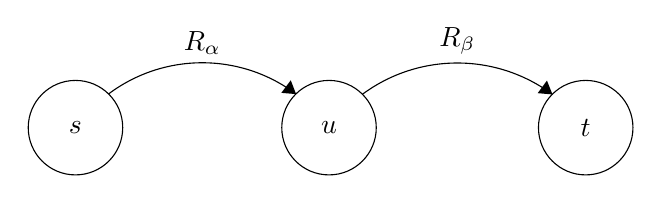
\begin{tikzpicture}[scale=0.2] \tikzstyle{every node}+=[inner sep=0pt] \draw [black] (21.4,-15.1) circle (3); \draw (21.4,-15.1) node {$s$}; \draw [black] (37.5,-15.1) circle (3); \draw (37.5,-15.1) node {$u$}; \draw [black] (53.8,-15.1) circle (3); \draw (53.8,-15.1) node {$t$}; \draw [black] (23.492,-12.966) arc (126.89872:53.10128:9.923); \fill [black] (35.41,-12.97) -- (35.07,-12.09) -- (34.47,-12.89); \draw (29.45,-10.48) node [above] {$R_\alpha$}; \draw [black] (39.613,-12.986) arc (126.52967:53.47033:10.141); \fill [black] (51.69,-12.99) -- (51.34,-12.11) -- (50.75,-12.91); \draw (45.65,-10.49) node [above] {$R_\beta$}; \end{tikzpicture} \end{center}

Al seguente grafo:

\definecolor{cffffff}{RGB}{255,255,255}
\begin{tikzpicture}[y=0.80pt,x=0.80pt,yscale=-1, inner sep=0pt, outer sep=0pt]   \path[cm={{0.58805,0.0,0.0,0.68269,(24.31388,102.98422)}},draw=black,fill=cffffff]     (156.7931,87.4161)arc(0.000:180.000:50.387171 and     44.750)arc(-180.000:0.000:50.387171 and 44.750) -- cycle;   \path[fill=black] (82.20771,167.96637) node[above right] (text3755) {s};   \path[cm={{0.74795,0.0,0.0,0.85608,(68.60394,12.42678)}},draw=black,fill=cffffff]     (265.1861,106.6421)arc(0.000:180.000:73.920640 and     42.098)arc(-180.000:0.000:73.920640 and 42.098) -- cycle;   \path[fill=black] (180.73416,65.26226) node[above right] (text3763) {U};   \path[draw=black,line join=miter,line cap=butt,line width=0.800pt]     (110.0523,145.4256) -- (164.8679,122.9266);   \path[cm={{0.71337,0.0,0.0,0.47229,(79.07095,130.99431)}},draw=black,fill=cffffff]     (265.1861,106.6421)arc(0.000:180.000:73.920640 and     42.098)arc(-180.000:0.000:73.920640 and 42.098) -- cycle;   \path[draw=black,line join=miter,line cap=butt,line width=0.800pt]     (113.3671,174.5960) -- (163.5672,177.9203);   \path[shift={(-12.0,0)},draw=black,fill=cffffff]     (236.0157,85.7587)arc(-0.038:180.038:13.922)arc(-180.038:0.038:13.922) --     cycle;   \path[cm={{0.92174,0.0,0.0,0.92174,(-3.13845,9.35718)}},draw=black,fill=cffffff]     (245.2972,119.5699)arc(-0.021:180.021:14.916721 and     12.596)arc(-180.021:0.021:14.916721 and 12.596) -- cycle;   \path[fill=black] (200,89.362183) node[above right] (text3817) {u1};   \path[fill=black] (200.91348,124.35682) node[above right] (text3817-5) {u2};   \path[fill=black] (124.37474,126.52254) node[above right] (text3842) {$R_\alpha$};   \path[fill=black] (127.6106,171.96516) node[above right] (text3846) {$R_\alpha$};   \path[cm={{0.8212,0.0,0.0,0.49268,(188.32152,21.20068)}},draw=black,fill=cffffff]     (265.1861,106.6421)arc(0.000:180.000:73.920640 and     42.098)arc(-180.000:0.000:73.920640 and 42.098) -- cycle;   \path[cm={{0.8212,0.0,0.0,0.42066,(180.68016,98.39161)}},draw=black,fill=cffffff]     (265.1861,106.6421)arc(0.000:180.000:73.920640 and     42.098)arc(-180.000:0.000:73.920640 and 42.098) -- cycle;   \path[draw=black,line join=miter,line cap=butt,line width=0.800pt]     (222.6493,122.0455) -- (286.4164,133.7944);   \path[draw=black,line join=miter,line cap=butt,line width=0.723pt]     (221.3768,77.3255) -- (285.5725,77.2936);   \path[shift={(99.17758,-11.35244)},draw=black,fill=cffffff]     (236.0157,85.7587)arc(-0.038:180.038:13.922)arc(-180.038:0.038:13.922) --     cycle;   \path[cm={{0.92174,0.0,0.0,0.92174,(102.03913,32.00475)}},draw=black,fill=cffffff]     (245.2972,119.5699)arc(-0.021:180.021:14.916721 and     12.596)arc(-180.021:0.021:14.916721 and 12.596) -- cycle;   \path[fill=black] (315.17758,78.00975) node[above right] (text3817-0) {t1};   \path[fill=black] (306.09106,147.00439) node[above right] (text3817-5-7) {t3};   \path[shift={(139.67676,-10.5883)},draw=black,fill=cffffff]     (236.0157,85.7587)arc(-0.038:180.038:13.922)arc(-180.038:0.038:13.922) --     cycle;   \path[cm={{0.92174,0.0,0.0,0.92174,(142.53831,32.76888)}},draw=black,fill=cffffff]     (245.2972,119.5699)arc(-0.021:180.021:14.916721 and     12.596)arc(-180.021:0.021:14.916721 and 12.596) -- cycle;   \path[fill=black] (353.67676,78.773872) node[above right] (text3817-6) {t2};   \path[fill=black] (346.59024,147.76852) node[above right] (text3817-5-6) {t4};   \path[fill=black] (326.2858,46.646969) node[above right] (text3942) {T1};   \path[fill=black] (324.32019,122.09327) node[above right] (text3942-3) {T2};   \path[fill=black] (248.34399,146.86179) node[above right] (text3990) {$R_\beta$};   \path[fill=black] (253.16176,74.356461) node[above right] (text3990-7) {$R_\beta$};   \path[fill=black,line join=miter,line cap=butt,line width=0.800pt] (0,0)     node[above right] (flowRoot4015) {};   \path[draw=black,line join=miter,line cap=butt,line width=0.800pt]     (401.1048,36.8263) .. controls (409.7612,32.3735) and (435.8124,31.6775) ..     (440.0757,44.4676) .. controls (444.4570,57.6116) and (438.5475,69.8092) ..     (438.5475,84.2027) .. controls (438.5475,89.4537) and (452.1943,92.7158) ..     (448.4812,96.4288) .. controls (445.2189,99.6911) and (435.7460,104.0714) ..     (438.5475,112.4757) .. controls (442.6528,124.7916) and (450.2611,160.1129) ..     (443.8964,172.8424) .. controls (440.9921,178.6510) and (417.3816,176.6631) ..     (411.0386,176.6631);   \path[fill=black] (462.52805,101.66471) node[above right] (text4174) {T};
\end{tikzpicture}\\


Bisogna cambiare anche la Relazione di iterazione nel seguente modo:

$R_{\alpha^{*}}\equiv\underset{n\geq0}{\bigcup}R_{\alpha}^{n}$ con
$R_{\alpha}^{0}=\{(s,\,\{s\})\,|\, s\in S\}$ e $R_{\alpha}^{n}=R_{\alpha}\circ\, R_{\alpha}^{n-1}$ 

Inoltre si introduce la relazione di combinazione, ossia quella che
traduce il parallelismo (l'operatore intersezione):

$(s,\, T)\in R_{\alpha}\otimes R_{\beta}\iff T=U\cup V\,\wedge\,(s,U)\in R_{\alpha}\,\wedge\,(s,V)\in R_{\beta}$

Tutto il resto è definito allo stesso modo di prima, a meno di stare
attenti agli insiemi di stati, anzichè agli stati.


\include{\string"contents/8-classica multimodale/class-multi\string"}

\begin{savequote}[50mm]
---Non so spiegarlo chiaramente, perchè non è chiaro neanche a me---
\qauthor{Alice} \end{savequote}


\chapter{Logiche Descrittive	}


\section{Introduzione - Logica AL}

Le DL sono una famiglia di logiche per la rappresentazione della conoscenza
che possono essere utilizzate per rappresentare conoscenza terminologica,
dando ad essa una semantica formale ben definita.

Un sistema di rappresentazione della conoscenza (KR) fornisce i mezzi
per definire, gestire, manipolare e ragionare su basi di conoscenza
(KB).

In una KB ci sono T-Box e A-Box

I TBox descrivono la terminologia della KB (concetti, ruoli atomici
e concetti composti), gli ABox sono asserzioni su individui della
KB

TBox es. $Madre\equiv Donna\sqcap Genitore$

ABox es. $Donna(Paola)$\\


La famiglia di logiche descrittive più utilizzata è la famiglia AL
(Attributive Language).

Nella logica AL (logica descrittiva tra le più semplici) ci sono:
\begin{description}
\item [{A,B,C}] concetti
\item [{R}] ruoli
\item [{		$\neg$}] negazione (solo di concetti atomici)
\item [{$\sqcap$}] di concetti
\item [{\textmd{I}}] concetti sono:\end{description}
\begin{itemize}
\item Concetti atomici A,B
\item $\top$, $\bot$
\item negazione di concetti atomici: $\neg A$
\item and di concetti: $C\sqcap D$
\item quantificazioni: $\forall R.C$, $\exists R.\top$
\end{itemize}
Un'interpretazione I di una base di conoscenza\'{ }e una coppia $I=<\Delta^{i},\cdot^{I}>$
composta da un dominio di interpretazione $\Delta$I, detto dominio
di I e da una funzione di interpretazione $\cdot^{I}$ che associa:

ad ogni \textbf{nome} di individuo un elemento: 

$a^{I}\in\Delta^{I}$

ad ogni \textbf{concetto} C un sottoinsieme di $\Delta^{I}$

$I:\ C\rightarrow C^{I}\subseteq\Delta^{I}$

e ad ogni \textbf{ruolo} un sottoinsieme di $\Delta$I \texttimes{}
$\Delta$I :

$R:\ R^{I}\subseteq\Delta^{I}\times\Delta^{I}$

I rouli sono quindi relazioni binarie, una volta interpretati

es. $(Peter,\ Chris)^{I}\in HaFiglio^{I}$

		

Inoltre:

$\bot^{I}=\emptyset$, $\top^{I}=\Delta^{I}$

$(C\sqcap D)^{I}=C^{I}\cap D^{I}$

$(\forall R.C)^{I}=\{a^{I}\in\Delta^{I}:\ (a^{I},b^{I})\in R^{I}\implies b^{I}\in C^{I}$\} 

es. $\forall Possiede.Cosa$ cioè se a possiede un oggetto del dominio
quello deve essere una cosa (slavery is bad)

$(\exists R.C)^{I}=\{a^{I}\in\Delta^{I}:\ \exists b\in\Delta^{I}:\ (a^{I},b^{I})\in R^{I}\wedge b^{I}\in C^{I}\}$\\


es. $\exists HaFiglio.Femmina$ cioè l'insieme dei genitori con una
figlia femmina\\



\subsection{Varianti di AL}

Indebolendo la logica AL si ottengono le logiche poco descrittive
della famiglia FL:
\begin{itemize}
\item F L- è ottenuta da AL eliminando la negazione atomica •
\item FL0 è ottenuta da FL- eliminando anche la quantificazione esistenziale
\end{itemize}
La logica AL può essere estesa aggiungendo alcuni costruttori: 
\begin{itemize}
\item costrutto $\mathcal{U}$ disgiunzione dei concetti $C\sqcup D$
\item costrutto $\mathcal{E}$ quantificazione esistenziale qualificata
$\exists R.C$
\item costrutto $\mathcal{C}$ complemento di concetti complessi $\neg C$
\item costrutto $\mathcal{N}$ cardinalità di un ruolo 
\end{itemize}
$(\leq nR)^{I}=\{a^{I}:\ \cardinal{\{b^{I}:\ (a^{I},b^{I})\in R^{I}\}}<n\}$

es. $(\leq2HaFiglio)^{I}$ è l'insieme delle persone un numero di
figli minore o uguale a 2.


\section{Confronti fra logiche }

In modo analogo a quanto si era fatto con le logiche derivate da K,
denotiamo con ALX la logica AL a cui si aggiunge il costrutto X


\subsection{Equivalenza $\alue$ed $\alc$}

Dimostriamo che $AL\mathcal{UE}\equiv AL\mathcal{C}$\\


IP) $\mathcal{UE}$

Ts)$\mathcal{C}$\\


Si vuole mostrate che a partire in$AL\mathcal{UE}$ posso fare tutto
ciò che faccio in $AL\mathcal{C}$, il che si riduce a mostrare che
in $\alue$posso fare negazioni di concetti qualsiasi.

Questo è immediato per i concetti atomici la cui negazione è per definizione
in $AL$

$\neg\top\equiv\bot$, $\neg\bot\equiv\top$

Per negare l'and di due concetti:

$\neg(D\sqcap E)\equiv\neg D\sqcup\neg E$ che sono concetti più semplici
di cui ricorsivamente posso costruire la negazione

$\neg\forall R.C\equiv\exists R.\neg C$

Con queste semplici trasformazioni posso rendere ricorsivamente più
semplice una qualsiasi formula di $\alc$ fino a portarla in una formula
di $\alue$\\
\\
IP) $\mathcal{C}$

Ts)$\mathcal{UE}$\\


Sfruttando De Morgan possiamo scrivere:

$D\sqcup E\equiv\neg(\neg D\sqcap\neg E)$

$\exists R.C\equiv\neg(\forall R.\neg C)$


\subsection{Confronto con logica del prim'ordine}

È possibile vedere le logiche AL, ALC, ALN, (deve essere con identità
nel caso di N)
\begin{itemize}
\item A è un concetto: $a(x)$
\item R è un ruolo: $R(x,y)$
\item $a\ $è un individuo: $a$ è una costante
\end{itemize}
Notiamo che ci sono due sole variabili libere e il dominio è fissato
(controllare) la logica del prim'ordine è decidibile.
\begin{description}
\item [{$\neg C$:}] $\neg C(x)$
\item [{$C\sqcap D\mathbf{:}$}] \foreignlanguage{english}{$C(x)\vee D(x)$}
\item [{$\forall R.C$:}] $\forall y:(R(x,y)\implies C(y)$)
\item [{$\exists R.C:$}] $\exists y:(R(x,y)\implies C(y))$
\item [{$\leq nR$$,$}] la logica deve essere con unità cioè avere un
predicato di uguaglianza E
\item [{$\exists x_{1},\ x_{2},...,\ x_{n+1}(R(x,x_{1})\wedge R(x,x_{2})\wedge\dots R(x,x_{n})$}] $\implies E(x_{1},x_{2})\vee E(x_{1},x_{2})\vee\dots..\underset{1\leq i\leq j\leq n+1}{\bigvee}E(x_{i},x_{j})$
\end{description}

\subsection{Confronto con logica multimodale}

\noindent L'espressività di ALC è la stessa di $K_{n}$ 

\noindent Infatti ogni ruolo $R_{i}$ si può mettere in corrispondenza
con $[R_{i}]c$


\section{Terminologia}
\begin{itemize}
\item Definizione: 
\end{itemize}
Una definizione associa a un concetto atomico un concetto complesso
(non atomico) es. $Parent\equiv Father\sqcup Mather$, il concetto
atomico viene detto anche simbolo nominale
\begin{itemize}
\item Simbolo di base (o nominale):
\end{itemize}
I ruoli e i concetti che appaiono solo nelle parti destre delle definizioni
\begin{itemize}
\item Interpretazione di base:
\end{itemize}
Un'interpretazione di una T-Box che interpreta solo i simboli di base
\begin{itemize}
\item Aciclico:
\end{itemize}
Nessun simbolo nominale usa sé stesso
\begin{itemize}
\item T-Box definitorio:
\end{itemize}
La sua interpretazione si estende in modo unico a una interpretazione
di tutto il t-box (estesa)

Un T-Box è definitorio se è possibile costruirne uno equivalente ma
aciclico\\


Non sono definitorie alcune T cicliche es.

$Human\equiv Animal\sqcap\forall hasParent.Human$\\


Ma alcune T cicliche sono definitorie es.

$A\equiv B\sqcap\exists R.(A\sqcap\neg A)$ che è equivalente a:

$A\equiv B\sqcap\exists R.(\bot)$ 


\section{Terminologia generalizzata}

A volte è possibile aggiungere nuovi operatori qua descritti.

\textbf{Inclusione}

Si possono usare T-Box del tipo:

$A\sqsubseteq B$ che vale se e solo se $A^{I}\subseteq B^{I}$

Una terminologia T generalizzata (cioè che contiene assiomi di inclusione)
può essere tradotta in una forma T normalizzata sostituendo le forme
del tipo:

$Woman\sqsubseteq Person$ con $Woman\mbox{\ensuremath{\equiv}}\underline{Woman}\sqcap Person$
dove $\underline{Woman}$ è un nuovo simbolo base (che denota qualità
specifiche)

In termini di espressività, le due forme sono equivalenti

Ogni modello di $T$ è anche modello di $\underline{T}$

Qualsiasi interpretazione base di un modello di $T$ è anche interpretazione
base di un modello di $\underline{T}$

Così facendo si ha che: $Woman^{I}\subseteq Person^{I}$ e quindi
$Woman^{I}\equiv Person\cap(\underline{Woman})^{I}$

\textbf{Set}

$Set{a_{1},a_{2},\dots,a_{n}}^{I}=\{a_{1}^{I},a_{2}^{I},\dots,a_{n}^{I}\}$

\textbf{Fills}

$Fills\ r\ c$ sono gli individui che sono in relazione tramite $r$
agli individui identificati da $c$

es. $FILLS\ :\ Child\ Chris$ sono tutti gli individui con figlio
``Chris''

$(Fills\ R:a)^{I}=\{b\in\Delta^{I}\;:\ (a^{I},b^{I})\in R^{I}\}$


\subsection{Note}

$\exists R.C$ si può sostituire con $\exists R.Set(a)$

Posso pensare i T-Box come composti solo di definizioni

Il T-Box può essere tolto del tutto specificando completamente le
definizioni nell'A-Box

Normalmente nelle Logiche Descrittive si fa l'UNA: l'unicity name
assunction cioè si assume che se si usano due nomi come a, b, allora
$a^{I}\neq b^{I}$


\section{Servizi di Reasoning}

I servizi di reasoning si propongono di risolvono quattro tipi di
problemi

\textbf{Soddifisfacibilità: }Un concetto C si dice soddisfacibile
rispetto al T-Box T se esiste un modello di T tale che $C^{I}$ non
è vuoto

\textbf{Sussunzione: }Un concetto C è sussunto da un concetto D, in
T se $C^{I}\subseteq D^{I}$ per ogni modello di T

\textbf{Equivalenze: }Due concetti C e D si dicono equivalenti rispetto
a T se $C^{I}=D^{I}$per ogni modello di T

\textbf{Disgiunzione: }Due concetti C e D sono disgiunti rispetto
a T se $C^{I}\cap D^{I}=\emptyset$ per ogni modello di T

Mostriamo che una KB che fornisce il servizio di sussunzione risolve
anche gli altri tre problemi, infatti:\\


$C$ è insoddisfacibile se e solo se $\bot\sqsubseteq C$ 

$C,D$sono equivalenti se $C\sqsubseteq D$ e $D\sqsubseteq C$

$C,D$sono disgiunti se $C\sqcap D\sqsubseteq\bot$


\section{Feauture Logic}

Le logiche descrittive più semplici appartengono alla famiglia della
features logics (FL in breve) e sono ottenute indebolendo la più\'{ }famosa
logica AL inibendo i costruttori di concetto più complessi.

La più semplice di queste è $FL_{0}$ che si ottiene da AL togliendo
$\bot$ e $\exists$

Un concetto in \textbf{forma normale }è del tipo:

$A_{1}\sqcap A_{2}\sqcap\dot{\dots A_{n}\forall R_{1}.C_{1}\sqcap\forall R_{2}.C_{2}\dots\sqcap\forall R_{m}.C_{m}}$

dove $C_{j}$ sono concetti in forma normale e $R_{j}$ sono ruoli
atomici\\


Posso scrivere qualsiasi concetto in questo modo con l'accortezza
di:

togliere i duplicati: $A_{i}\neq A_{j}$

``sciogliere'' i ruoli con intersezioni: 

$\forall R.(C\sqcap D)\equiv\forall R.C\sqcap\forall R.D$

	

Siano C e D due concetti $FL_{0}$ in forma normale: \\


$C\equiv A_{1}\sqcap\dots\sqcap A_{m}\sqcap\forall R1.C1\sqcap\forall Rn.Cn$

$D\equiv B1\sqcap\dots\sqcap Bk\sqcap\forall S1.D1\sqcap\forall Sl.Dl$	\\


allora $C\sqsubseteq D$ se e solo se \\


1. per ogni i, $1\leq i\leq k$ esiste un j, $1\leq j\leq m$ per
il quale $Bi=Aj$.

2. per ogni i, $1\leq i\leq l$ esiste un j, $1\leq j\leq n$ per
il quale $Si=Rj$ e$Cj\sqsubseteq Di$.


\subsection{Varianti}

Ad $AL_{0}$può essere aggiunto il concetto $\bot$, ottenendo $AL_{\bot}$e
la forma normale viene a essere la stessa di prima a cui si aggiunge
l'opportunità per un concetto di essere o$\bot$

Notiamo che $\bot\sqsubseteq C$, per ogni $C$

Ad $AL_{0}$ si può aggiungere la negazione di concetti atomici ottenendo
$AL_{\neg}$

Notiamo che $\bot\equiv A\wedge\neg A$, quindi $AL_{\neg}$contiene
strettamente$AL_{0}$	

In $ALC$ per verificare se $C\sqsubseteq D$ possiamo controllare
che $C\sqcap\neg D$ si insoddisfacibile

Per controllare $C\equiv D$ possiamo quindi testare $C\sqcap\neg D$
e $D\sqcap\neg C$.


\section{A-Box Reasoning}

	I servizi di reasoning di A-Box sono:

\textbf{Consistenza}: Un A-Box è consistente in un modello T-Box T
se c'è un'interpreatzione che sia modello sia di T che di A

\textbf{Instance Checking}: Un individuo è istanza di un concetto
C rispetto a un A-Box A se è membro dell'insieme C. $\vera A{C(a)}$
il che vale se e solo se $A\cup\{\neg C(a)\}$ è insoddisfacibile

\textbf{Instance Retrivial}: Trova tutti gli individui che sono istanze
di una data descrizione

\textbf{Problema di Realizzazione}: Trova il concetto più specifico
a cui un individuo appartiene


\subsection{Variante}

T-Box ed A-Box si possono arricchire con $C\implies D$ cioè: per
ogni individuo $a$ cui è noto $C(a)$ si ha anche $D(a)$.

Notiamo che NON vale $\neg D\implies\neg C$

		


\begin{savequote}[50mm]
---Bu-burro, certo, ci vuole un po' di burro! Buuuurro!--- \\
---Bu-bu-burro? Eccolo!--- \\
---Oh, grazie! Burro! Benissimo!---
\qauthor{Lewis Carroll} \end{savequote}


\chapter{Logica Modale Del Prim'Ordine}


\section{La Sintassi delle Logiche Modali del Prim'Ordine}

Una logica modale del prim'ordine è definita sul seguente alfabeto:
\begin{itemize}
\item Costanti $(k_{1},...,k_{n})$
\item Variabili $(x_{1},...,x_{n})$
\item Lettere predicative $A_{i}^{j}$
\item Connettivi logici: $\neg,\,\wedge,\,\vee,\,\implies,\,\iff$
\item Quantificatori universali ed esistenziali: $\forall x_{i},\,\exists x_{i}$
\item Connettivi modali $\square,\,\diamond$
\item Parentesi ), (
\end{itemize}
Si chiamano termini le costanti e le lettere predicative, gli indichiamo
come $t_{i}$

Si chiamano formule atomiche, le formule del tipo:

$A_{i}^{n}(t_{1},...,\, t_{n})$

Le formule ben formate sono definite come al solito:
\begin{itemize}
\item Le formule atomiche sono formule ben formate
\item $a,\,\neg a,\,(\forall x)a,\,(\exists x)a,\,\boa,\,\dia$ sono furmule
ben formate
\item $a,\, b,\,(a\wedge b),\,(a\vee b),\,(a\implies b),\,(a\iff b)$ sono
formule ben formate
\item Null'altro è una formula ben formata.
\end{itemize}

\section{Semantica della Logica Modale del Prim'Ordine}


\subsection{Frame e modello}

Definiamo un frame della logica modale del prim'ordine il seguente:

F = (S, R, D)

in cui:
\begin{itemize}
\item S è insieme dei possibili stati
\item R è la relazione di raggiungibilità tra gli stati
\item D è la funzione che associa a ogni stato il suo dominio.
\end{itemize}
Chiamiamo modello il seguente:

$\mu=(S,\, R,\, D,\, I)$

dove I è la funzione di interpretazione, che può essere vista come
l'unione di due funzioni separate:
\begin{itemize}
\item $I_{c}$ è la funzione di interpretazione delle costanti, ossia che
in ogni stato associa al valore di una costante un valore del dominio
in quello stato
\item $I_{P}$ è la funzione di interpretazione dei predicati, che associa
a un predicato una relazione n-aria tra gli elementi del dominio
\end{itemize}

\subsection{Tipi di dominio}

I domini nella logica modale del pr'imordine possono essere visti
in verie maniere differenti, a seconda che gli stati abbiano domini
uguali o diversi tra loro.

In generale, infatti ogni stato potrebbe avere domini a piacere differenti.

Si dicono domini costanti quei domini per cui vale:

$\forall\alpha,\beta\in S\, D_{\alpha}=D_{\beta}$

Si dicono domini variabili monotoni i domini per cui vale:

$\forall\alpha,\beta\in S\, D_{\alpha}\subseteq D_{\beta}$

Si dicono domini variabili antimonotoni i domini per cui vale:

$\forall\alpha,\beta\in S\, D_{\alpha}\supseteq D_{\beta}$

I domini monotoni sono i domini in cui ``nulla si crea'', mentre
i domini antimonotoni sono quelli in cui ``nulla si distrugge''.
Un dominio costante è sia monotono che antimonotono, per cui gli elementi
dell'insieme rimangono immutabili.

Se chiamiamo P l'insieme dei predicati, C l'insieme delle costanti,
e $R_{D}$ l'insieme di tutte le possibili relazioni sui domini D,
possiamo definire l'interpretazione I come:

$I_{c}:\, C\times S\longrightarrow D$

$I_{P}:\, P\times S\longrightarrow R_{D}$

In questo caso si parla di logica a designatori non rigidi.

Se invece consideriamo una logica a designatori non rigidi abbiamo
I definita come:

$I_{c}:\, C\longrightarrow D$

$I_{P}:\, P\longrightarrow R_{D}$


\subsection{Semantica}

Chiamiamo s la funzione di assegnamento, posto V l'insieme delle variabili
ossia la funzione, è la seguente:

$s:\, V\times S\longrightarrow D$

è possibile estendere s ad s{*}, e se chiamiamo T l'insieme di tutti
i possibili termini, abbiamo che:

$s*:\, T\times S\longrightarrow D$

che è così definita:

$s*(x_{i})=s(x_{i})$

$s*(k_{i})=I(k_{i})$

Indichiamo che una formula è vera in un modello $\mu$, rispetto all'assegnamento
s, in un mondo $\alpha$ nel seguente modo:

$\veraw{\mu,s}{\alpha}a$

La verità di una formula è definita per induzione sui connettivi minimi:
\begin{itemize}
\item $\veraw{\mu,s}{\alpha}{A_{i}^{n}(t_{1},...,t_{n})\iff(s*(t_{1}),...,s*(t_{n}))\in I_{P}(A_{i}^{n},\alpha)}$
\item $\veraw{\mu,s}{\alpha}{\neg b}\iff\nonveraw{\mu,s}{\alpha}b$
\item $\veraw{\mu,s}{\alpha}{b\implies c}\iff\veraw{\mu,s}{\alpha}{c\,\vee\,\nonveraw{\mu,s}{\alpha}b}$
\item $\veraw{\mu,s}{\alpha}{(\forall x)b}\iff(\forall s'\,:\, s'(x)\not=s(x)\,\wedge\, s'(x_{i})=s(x_{i}))\,\veraw{\mu,s}{\alpha}{(\forall x)b}$
\item $\veraw{\mu,s}{\alpha}{\boxx b}\iff\forall\beta\,:\,(\alpha,\,\beta)\in R\,\veraw{\mu,s}{\beta}b$
\end{itemize}
Una formula M è vera in un mondo se ogni assegnamento la soddisfa,
insoddisfacibile se nessuno la sofddisfa e sodisfacibile se è vera
per alcuni assegnamenti.

Una formula si dice vera in un modello se è vera in tutti i mondi
del modello

Una formula si dice valida in un frame se è vera in tutti i modelli
costruiti su quel frame.


\section{Assiomatizzazzione della Logica Modale del Prim'Ordine}


\subsection{Gli Assiomi della logica del prim'ordine}

Gli assiomi della logica del prim'ordine sono:
\begin{itemize}
\item A1: $a\implies(b\implies a)$
\item A2: $(a\implies(b\implies c))\implies((a\implies b)\implies(a\implies c))$
\item A3: $(\neg a\implies\neg b)\implies((\neg a\implies b)\implies a)$
\item A4: $(\forall x)a(x)\implies a[t/x]$, dove t è un termine libero
per x in A(x)
\item A5: $(\forall x)(a\implies b)\implies(a\implies(\forall x)b)$, purchè
non ci siano occorrenze libere di x in A
\end{itemize}
Inoltre valgono le due regole di inferenza:
\begin{itemize}
\item MP: $\dfrac{a,\, a\implies b}{b}$
\item Gen: $\dfrac{a}{(\forall x)a}$
\end{itemize}

\subsection{Formula di Barcan}

Si chiama formula di barcan la seguente formula:

$(\forall x)\boa\implies\boxx{(\forall x)a}$

o equivalentemente la sua duale:

$\diam{(\exists x)a\implies(\exists x)\dia}$

Si chiama formula di barcan inversa la formula:

$\boxx{(\forall x)a}\implies(\forall x)\boa$

o equivalentemente la sua duale:

$(\exists x)\dia\implies\diam{(\exists x)a}$

La formula di barcan vale se e solo se il modello è antimonotono,
la formula di barcan inversa vale se e solo se il modello è monotono.

Quindi in un modello a designatori costanti vale la formula di barcan
inversa.


\subsection{Minima logica modale del prim'ordine}

Se consideriamo la logica che usa tutti gli assiomi della logica modale
e quella del prim'ordine, ossia una logica che usa i seguenti assiomi:
\begin{itemize}
\item A1, A2, A3
\item A4, A5
\item K
\end{itemize}
E le seguenti regole di inferenza:
\begin{itemize}
\item MP
\item Gen
\item RN
\end{itemize}
Otteniamo la minima logica modale del prim'ordine.

Si può dimostrare che in questa logica vale la formula di Barcan inversa:

$\teorema{(\forall x)a\implies a}$ -- per A4, t = x

$\teorema{\boxx{((\forall x)a\implies a)}}$ -- per RN

$\teorema{\boxx{((\forall x)a\implies a)\implies(\boxx{(\forall x)a}\implies\boa)}}$
-- per K

$\teorema{\boxx{(\forall x)a}\implies\boa}$ -- per MP

$\teorema{(\forall x)(\boxx{(\forall x)a}\implies\boa)}$ -- per Gen

$\teorema{(\forall x)(\boxx{(\forall x)a}\implies\boa)}\implies(\boxx{(\forall x)a}\implies(\forall x)\boa)$
-- per A5 

$\teorema{\boxx{(\forall x)a}\implies(\forall x)\boa}$ -- per MP

che è la formula di barcan inversa.

Allo stesso modo si può dimostrare che aggiungendo lo schema:

B: $a\implies\boxx{\dia}$

Dalla minima logica modale del prim'ordine si ricava anche la formula
di Barcan. Questo è vero intuitivamente perchè se ho una relazione
simmetrica monotona, allora deve anche essere antimonotona, e questo
può essere vero solo se ci troviamo nel caso a domini costanti.

Si può usare, anzichè la logica normale, una logica classica, e si
possono ricavare logiche in cui le due formule di Barcan non valgano.



\chapter{Bisimulazione}


\section{Definizione di bisimulazione}

Siano $\mu=(S,\, R,\, V)$ e $\mu'=(S',\, R',\, V')$ due modelli
e siano $s\in S$, e $t\in S'$ due stati

Si dice che le coppie $(\mu,\, s)$ e $(\mu',\, s)$ sono in bisimulazione
tra loro, ossia:

$(\mu,\, s)\leftrightarroweq(\mu',\, s)$

Se esiste una relazione $E:S\times S$ tale che
\begin{enumerate}
\item $(s,\, t)\in E$
\item se $(x,\, y)\in E$ allora:\\
a)$\forall P\in\phi\, x\in V(P)\iff y\in V'(P)$\\
b1)$(x,\, z)\in R\implies\exists u\in S'\,:\,(y,\, u)\in R'\,\wedge\,(z,\, u)\in E$\\
b2)$(y,\, u)\in R'\implies\exists z\in S\,:\,(x,\, z)\in R\,\wedge\,(z,\, u)\in E$
\end{enumerate}
Due frame sono in bisimulazione se soddisfano le condizioni 1, b1
e b2.


\subsection{Teorema}

se $(\mu,\, s)\leftrightarroweq(\mu',\, s)$

allora: 

$\forall\varphi\in\phi\,\veraw{\mu}s{\varphi}\iff\veraw{\mu'}t{\varphi}$


\section{Esempi di bisimulazione}


\subsection{Alberi binari e Retta}

Consideriamo il frame rappresentante la lettera dei numeri naturali:

$N=(\mathbb{N},\, successivo)$

E il frame che rappresenta un albero binario a dimensione infinita:

$B=(w=\{0,\,1\}*,\,\rho)$

Supponiamo che V su B sia: 

$V(P)=\{w\in\{0,\,1\}*\,:\,|w|=2n\}$

Allora esiste una unica valutazione V' su N tale che $(B,\, V,\,0)\leftrightarroweq(N,\, V',\,\epsilon)$,
ed è:

$V'(P)=\mathbb{P}$ (l'insieme dei numeri pari)

Dimostriamolo per induzione:

$(n,\, w)\in E\iff|w|=n$

il caso base si dimostra banalmente:

$|\epsilon|=0$

$(\epsilon,\,0)\in E$

per definizione. Per il passo induttivo abbiamo:

$|w|=n$

$(w,\, n)\in E$

sia w per ipotesi tale che $|w|=n+1$

allora:

$w=ua$, $|u|=n$, $a\in\{0,\,1\}$

per la condizione 1 di bisimulazione:

$(u,\, w)\in\rho$ e $(u,\, n)\in E$

per la condizione b1 invece:

$\exists m\in\mathbb{N}\,:\, m=n+1\wedge(w,\, n+1)\in E$

e quindi si deduce facilmente che:

$|w|=|ua|=n+1$

e quindi la valutazione non può che essere la sola V', perché è quella
che si ricava imponendo la condizione di bisimulazione, e che rispetta
anche la condizione 2.

\begin{center} 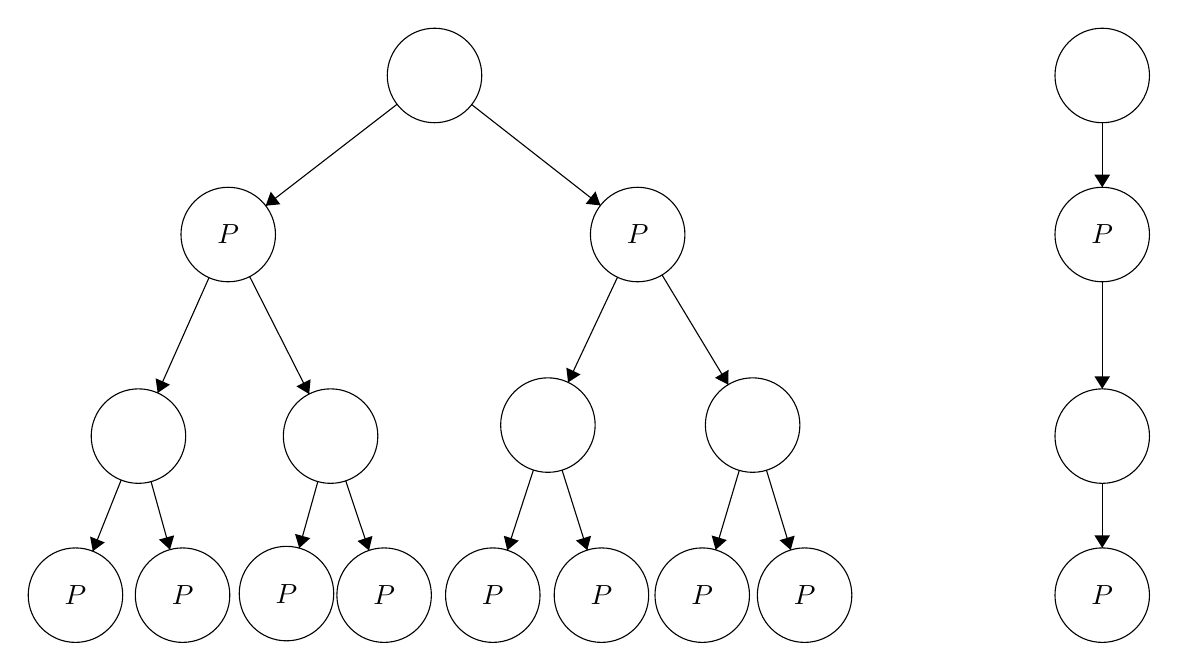
\begin{tikzpicture}[scale=0.2] \tikzstyle{every node}+=[inner sep=0pt] \draw [black] (26.2,-6.3) circle (3); \draw [black] (13.1,-16.4) circle (3); \draw (13.1,-16.4) node {$P$}; \draw [black] (39.1,-16.4) circle (3); \draw (39.1,-16.4) node {$P$}; \draw [black] (7.4,-29.2) circle (3); \draw [black] (19.6,-29.2) circle (3); \draw [black] (33.4,-28.5) circle (3); \draw [black] (46.4,-28.5) circle (3); \draw [black] (3.4,-39.3) circle (3); \draw (3.4,-39.3) node {$P$}; \draw [black] (10.2,-39.3) circle (3); \draw (10.2,-39.3) node {$P$}; \draw [black] (16.8,-39.2) circle (3); \draw (16.8,-39.2) node {$P$}; \draw [black] (23,-39.3) circle (3); \draw (23,-39.3) node {$P$}; \draw [black] (29.9,-39.3) circle (3); \draw (29.9,-39.3) node {$P$}; \draw [black] (36.8,-39.3) circle (3); \draw (36.8,-39.3) node {$P$}; \draw [black] (43.2,-39.3) circle (3); \draw (43.2,-39.3) node {$P$}; \draw [black] (49.7,-39.3) circle (3); \draw (49.7,-39.3) node {$P$}; \draw [black] (68.6,-6.3) circle (3); \draw [black] (68.6,-16.4) circle (3); \draw (68.6,-16.4) node {$P$}; \draw [black] (68.6,-29.2) circle (3); \draw [black] (68.6,-39.3) circle (3); \draw (68.6,-39.3) node {$P$}; \draw [black] (23.82,-8.13) -- (15.48,-14.57); \fill [black] (15.48,-14.57) -- (16.41,-14.48) -- (15.8,-13.68); \draw [black] (28.56,-8.15) -- (36.74,-14.55); \fill [black] (36.74,-14.55) -- (36.42,-13.66) -- (35.8,-14.45); \draw [black] (11.88,-19.14) -- (8.62,-26.46); \fill [black] (8.62,-26.46) -- (9.4,-25.93) -- (8.49,-25.53); \draw [black] (14.46,-19.07) -- (18.24,-26.53); \fill [black] (18.24,-26.53) -- (18.33,-25.59) -- (17.43,-26.04); \draw [black] (37.82,-19.11) -- (34.68,-25.79); \fill [black] (34.68,-25.79) -- (35.47,-25.28) -- (34.57,-24.85); \draw [black] (40.65,-18.97) -- (44.85,-25.93); \fill [black] (44.85,-25.93) -- (44.87,-24.99) -- (44.01,-25.5); \draw [black] (6.3,-31.99) -- (4.5,-36.51); \fill [black] (4.5,-36.51) -- (5.26,-35.95) -- (4.33,-35.58); \draw [black] (8.2,-32.09) -- (9.4,-36.41); \fill [black] (9.4,-36.41) -- (9.67,-35.5) -- (8.7,-35.77); \draw [black] (18.79,-32.09) -- (17.61,-36.31); \fill [black] (17.61,-36.31) -- (18.31,-35.68) -- (17.34,-35.41); \draw [black] (20.56,-32.04) -- (22.04,-36.46); \fill [black] (22.04,-36.46) -- (22.26,-35.54) -- (21.31,-35.86); \draw [black] (32.48,-31.35) -- (30.82,-36.45); \fill [black] (30.82,-36.45) -- (31.55,-35.84) -- (30.6,-35.53); \draw [black] (34.3,-31.36) -- (35.9,-36.44); \fill [black] (35.9,-36.44) -- (36.14,-35.53) -- (35.18,-35.83); \draw [black] (45.55,-31.38) -- (44.05,-36.42); \fill [black] (44.05,-36.42) -- (44.76,-35.8) -- (43.8,-35.51); \draw [black] (47.28,-31.37) -- (48.82,-36.43); \fill [black] (48.82,-36.43) -- (49.07,-35.52) -- (48.11,-35.81); \draw [black] (68.6,-9.3) -- (68.6,-13.4); \fill [black] (68.6,-13.4) -- (69.1,-12.6) -- (68.1,-12.6); \draw [black] (68.6,-19.4) -- (68.6,-26.2); \fill [black] (68.6,-26.2) -- (69.1,-25.4) -- (68.1,-25.4); \draw [black] (68.6,-32.2) -- (68.6,-36.3); \fill [black] (68.6,-36.3) -- (69.1,-35.5) -- (68.1,-35.5); \end{tikzpicture} \end{center}


\subsection{Alberi binari e frame finito}

Supponiamo di prendere su un frame binario B la seguente funzione
di valutazione:

$V(P)=\{0w\,|\, w\in\{0,1\}*\}$

$V(Q)=\{1w\,|\, w\in\{0,1\}*\}$

In questo frame Q è vera su tutto il sotto-albero destro, mentre P
sul scotolassero sinistro.

è evidente che non può esistere alcuna V' su N tale che $(B,\, V,\,0)\leftrightarroweq(N,\, V',\,\epsilon)$,
perché dovrebbero esistere due insiemi di stati non in relazione tra
loro per cui in uno valga P e nell'altro Q. Ma questo non è possibile,
poiché il frame N è una retta di elementi connessi a uno a uno. Tuttavia
esiste un frame molto più semplice e finito che bisimula l'albero,
di soli 3 stati, uno per lo stato $\epsilon$, uno per lo stato in
qui vale P, e uno per lo stato in cui vale Q. Si può vedere come l'automa
che riconosce se la stringa è ``etichettata'' P o Q.

\begin{center} \begin{tikzpicture}[scale=0.2] \tikzstyle{every node}+=[inner sep=0pt] \draw [black] (39.2,-9.7) circle (3); \draw [black] (25.5,-25.3) circle (3); \draw (25.5,-25.3) node {$P$}; \draw [black] (53,-25.3) circle (3); \draw (53,-25.3) node {$Q$}; \draw [black] (37.22,-11.95) -- (27.48,-23.05); \fill [black] (27.48,-23.05) -- (28.38,-22.77) -- (27.63,-22.11); \draw [black] (24.182,-27.982) arc (1.56859:-286.43141:2.25); \fill [black] (22.57,-25.89) -- (21.76,-25.41) -- (21.78,-26.41); \draw [black] (55.83,-26.26) arc (99:-189:2.25); \fill [black] (53.96,-28.13) -- (53.59,-29) -- (54.58,-28.84); \draw [black] (41.19,-11.95) -- (51.01,-23.05); \fill [black] (51.01,-23.05) -- (50.86,-22.12) -- (50.11,-22.79); \end{tikzpicture} \end{center} 


\subsection{Infiniti cammini vs Cammino infinito}

Consideriamo due frame, il primo tale che da un nodo $\alpha$ partono
infiniti percorsi, e l'altro che ha un solo percorso di lunghezza
infinita. 

\begin{center} 
\begin{tikzpicture}[scale=0.2] 
\tikzstyle{every node}+=[inner sep=0pt] 
\draw [black] (36,-8.8) circle (3); 
\draw (36,-8.8) node {$\alpha$}; 
\draw [black] (27.8,-21.8) circle (3); 
\draw [black] (22.6,-31.4) circle (3); 
\draw [black] (43.5,-21.1) circle (3); 
\draw [black] (50.4,-31.4) circle (3); 
\draw [black] (57.6,-41.3) circle (3); 
\draw (58.9,-15.2) node {$...$}; 
\draw [black] (12.1,-19.2) circle (3); 
\draw [black] (33.25,-10) -- (14.85,-18); 
\fill [black] (14.85,-18) -- (15.78,-18.14) -- (15.38,-17.23); 
\draw [black] (34.4,-11.34) -- (29.4,-19.26); 
\fill [black] (29.4,-19.26) -- (30.25,-18.85) -- (29.4,-18.32); 
\draw [black] (26.37,-24.44) -- (24.03,-28.76); 
\fill [black] (24.03,-28.76) -- (24.85,-28.3) -- (23.97,-27.82); 
\draw [black] (37.56,-11.36) -- (41.94,-18.54); 
\fill [black] (41.94,-18.54) -- (41.95,-17.6) -- (41.09,-18.12); 
\draw [black] (45.17,-23.59) -- (48.73,-28.91); 
\fill [black] (48.73,-28.91) -- (48.7,-27.96) -- (47.87,-28.52); 
\draw [black] (52.16,-33.83) -- (55.84,-38.87); 
\fill [black] (55.84,-38.87) -- (55.77,-37.93) -- (54.96,-38.52); 
\end{tikzpicture} 
\end{center} 

\begin{center} 
\begin{tikzpicture}[scale=0.2] 
\tikzstyle{every node}+=[inner sep=0pt] 
\draw [black] (36,-8.8) circle (3); 
\draw (36,-8.8) node {$\alpha'$}; 
\draw [black] (27.8,-21.8) circle (3); 
\draw [black] (22.6,-31.4) circle (3); 
\draw [black] (47.8,-16.7) circle (3); 
\draw [black] (57.6,-23.5) circle (3); 
\draw [black] (67.5,-30.7) circle (3); 
\draw (76,-36.8) node {$...$}; 
\draw [black] (14.4,-17.4) circle (3); 
\draw [black] (39.4,-23.5) circle (3); 
\draw [black] (33.21,-9.91) -- (17.19,-16.29); 
\fill [black] (17.19,-16.29) -- (18.12,-16.46) -- (17.75,-15.53); 
\draw [black] (34.4,-11.34) -- (29.4,-19.26); 
\fill [black] (29.4,-19.26) -- (30.25,-18.85) -- (29.4,-18.32); 
\draw [black] (26.37,-24.44) -- (24.03,-28.76); 
\fill [black] (24.03,-28.76) -- (24.85,-28.3) -- (23.97,-27.82); 
\draw [black] (38.49,-10.47) -- (45.31,-15.03); 
\fill [black] (45.31,-15.03) -- (44.92,-14.17) -- (44.36,-15); 
\draw [black] (50.26,-18.41) -- (55.14,-21.79); 
\fill [black] (55.14,-21.79) -- (54.76,-20.92) -- (54.19,-21.74); 
\draw [black] (60.03,-25.26) -- (65.07,-28.94); 
\fill [black] (65.07,-28.94) -- (64.72,-28.06) -- (64.13,-28.87); 
\draw [black] (69.94,-32.45) -- (73.56,-35.05); 
\fill [black] (73.56,-35.05) -- (73.2,-34.18) -- (72.62,-34.99); 
\draw [black] (36.68,-11.72) -- (38.72,-20.58); 
\fill [black] (38.72,-20.58) -- (39.03,-19.69) -- (38.06,-19.91); 
\end{tikzpicture} 
\end{center}

Si dimostra che non esiste una bisimulazione tra i due frame:

$(F,\,\alpha)\not\leftrightarroweq(F',\,\alpha')$

Dimostriamolo per assurdo, e supponiamo esista una bisimulazione tra
i due frame: 

$(F,\,\alpha)\leftrightarroweq(F',\,\alpha')$

supponiamo inoltre w accessibile da $\alpha'$ sul ramo infinito.

Poiché sono in condizione di bisimulazione vale la condizione b2:

$(\alpha',\, u)\in R'\implies\exists\beta\in F\,:\,(\alpha,\,\beta)\in R\,\wedge\,(\beta,\, w)\in E$

Ma poiché $\beta$ appartiene al primo frame, esso sta su un ramo
di lunghezza finita n.

Ma allora si ha che:

$\nonveraw F{\beta}{\diam{^{n}\top}}$

Tuttavia abbiamo anche che:

$\veraw{\forall n\in\mathbb{N},\, F'}{\beta}{\diam{^{n}\top}}$

ma non può essere perché i due frame sono in bisimulazione, assurdo!

quindi non può esistere una bisimulazione tra i due frame.


\subsection{Irriflessività e logica modale e temporale}

Non esiste alcuna formula modale temporale per esprimere l'irriflessività,
infatti siano:

$Z=(\mathbb{Z},<)$

$F=(W,\, R)$

con $R=\{(a,a)\}$ e $W=\{a\}$

Sia $V_{F}$ una generica valutazione su F, esiste sempre una $V_{Z}$
su Z tale che:

$(Z,\, V_{Z},\,0)\leftrightarroweq(F,\, V_{F},\, a)$

Infatti $\forall P\in\phi$ e $\forall n\in\mathbb{Z}$ sia:

$V_{Z}(P,\, N)=V_{F}(P,\, a)$ 

o meglio:

$V_{F}(P)=\{a\}\implies V_{Z}(P)=\mathbb{Z}$

E' facile provare che i due modelli sono in bisimulazione:

1) $E\subseteq\mathbb{Z}\times W,\,\forall n\in\mathbb{Z}\,(n,\, a)\in E$

b1) $n<m\implies(m,\, a)\in E\,\wedge\,(a,\, a)\in R$

b2) $(a,\, a)\in R\implies(n+1,\, a)\in E\,\wedge\, n<n+1$

Ma, poiché il frame Z è irriflessivo, se esistesse una formula che
esprime l'irriflessività, allora non sarebbe valida su F, ma ciò è
impossibile, perché è in bisimulazione con Z, e quindi tutte le formule
vere su F sono vere su Z e viceversa.



\chapter{Model Checking}


\section{Frame Temporale}

chiamiamo frame temporale un generico frame

$\tau=(T,\,<)$

dove < è una relazione irriflessiva e transitiva.

Posto V una funzione di valutazione, un modello su un frame temporale
è:

$\mu=(\tau,\, V)$

Le logiche basate sui frame temporali si chiamano logiche (modali)
temporali.

Il frame temporale può avere alcune proprietà, infatti si dice:
\begin{itemize}
\item Lineare a destra: $\forall x,y,z((x<y\,\wedge\, x<z)\implies(y<z\,\vee\, z<y\,\vee\, y=z))$ 
\item Lineare a sinistra: $\forall x,y,z((x>y\,\wedge\, x>z)\implies(y>z\,\vee\, z>y\,\vee\, y=z))$ 
\item Ramificato a destra: se non è lineare a destra
\item Ramificato a sinistra: se non è lineare a sinistra
\item Discreto: $\forall x,y(x<y\implies\exists z(x<z\,\wedge\,\neg\exists u(x<u\,\wedge\, u<z)))$
\item Denso: $\forall x,y(x<y\implies\exists z(x<z<y))$
\end{itemize}

\section{Logica LTL}


\subsection{Notazione modena}

La logica LTL ha una notazione più nuova rispetto a quella inizialmente
formulata con gli operatori $\square,\,\diamond,\,\circ$:
\begin{itemize}
\item $\mathcal{G}\equiv[F]$ chiamato ``globally''
\item $\mathcal{F}\equiv<F>$ chiamato ``eventaully''
\item $\mathcal{X}\equiv\circ$ chiamato next
\item $\mathcal{U}$ chiamato until
\item $\mathcal{R}$ chiamato release
\end{itemize}

\subsection{Operatori modali ed espressività della logica}

Dimostriamo Ora alcune proprietà degli operatori di LTL:
\begin{enumerate}
\item $\mathcal{X}$ può essere espresso da $\mathcal{U}$ 
\item $\mathcal{G}$ può essere espresso tramite il solo operatore  $\mathcal{U}$ 
\item $\mathcal{F}$ può essere espresso tramite il solo operatore $\mathcal{U}$ 
\item $\mathcal{X}$ non può essere espresso con $\mathcal{G}$ e $\mathcal{F}$ 
\end{enumerate}
Si dimostra abbastanza facilmente:

1) ricordando che next ha il significato seguente:

$\veraw{\mu}s{\next a}\iff\veraw{\mu}{s+1}a$

consideriamo la seguente formula:

$\veraw{\mu}n{\until{\bot}a}$

è vera se e solo se vale la seguente:

$\exists m>n(\veraw{\mu}ma\,\wedge\,\forall k(n<k<m\implies\veraw{\mu}k{\bot}))$

poichè $\veraw{\mu}k{\bot}$ è falsa in ogni mondo, deve essere falso
l'antecedente dell'implicazione, quindi non deve esistere nessun k
tale che $n<k<m$

Allora avremo che:

$m=n+1$

e quindi

$\veraw{\mu}n{\until{\bot}a}\iff\veraw{\mu}n{\next a}$

2 e 3) Possiamo esprimere l'eventually (e quindi il globally) facilmente
come:

$\eventually a\equiv\until{\top}a$

e quindi:

$\neg\globally{\neg a}\equiv\until{\top}a$

$\globally a\equiv\neg(\until{\top}{\neg a)}$

infatti:

$\veraw{\mu}s{\until{\top}a}\iff\exists t(s<t\,\wedge\,\veraw{\mu}ta\,\wedge\,\forall k(s<k<t\implies\veraw{\mu}k{\top})$

ma poichè $\forall k(s<k<t\implies\veraw{\mu}k{\top})$ è sempre vera,
perchè il conseguente è sempre vero, allora abbiamo:

$\exists t(s<t\,\wedge\,\veraw{\mu}ta)$

che è la definizione di eventually.

4) Supponiamo per assurdo che si possa esprimere l'operatore next
in funzione di globally e eventually.

allora prendiamo il frame:

$N=(\mathbb{N},\,<)$

e usiamo la seguente valutazione:

$V(P)=\{3n\,|\, n\in\mathbb{N}\}$

quindi il modello sarà:

$\mu=(N,\, V)$

allora, per ogni formula ben formata si ha che:

$\veraw{\mu}na\iff\veraw{\mu}{n+3}a$

e

$\veraw{\mu}1a\iff\veraw{\mu}2a$

Per dimostrarlo, uso la bisimulazione:
\begin{itemize}
\item $(\mu,\, n)\leftrightarroweq(\mu,\, n+3)$
\item $(\mu,\,1)\leftrightarroweq(\mu,\,2)$
\end{itemize}
Nel primo caso, costruisco E tale che:

$(n,\, m)\in E\iff m=n+3$

<\textcompwordmark{}<MANCA! non ci ho capito molto, pessimi appunti...>\textcompwordmark{}>


\section{Logiche per il model checking}


\subsection{Logiche per il model checking e semantica}

le principali logiche usate nel Model Checking sono 3:
\begin{itemize}
\item LTL, linear temporal logic (proposta da Pnueli nel 1977)
\item CTL, computational tree logic (proposta da clarkee emerson nel 1981)
\item CTL{*} (proposta da Emerson e Holpem nel 1986)
\end{itemize}
Le re logiche sono in relazione tra loro nel modo seguente:

\begin{center} 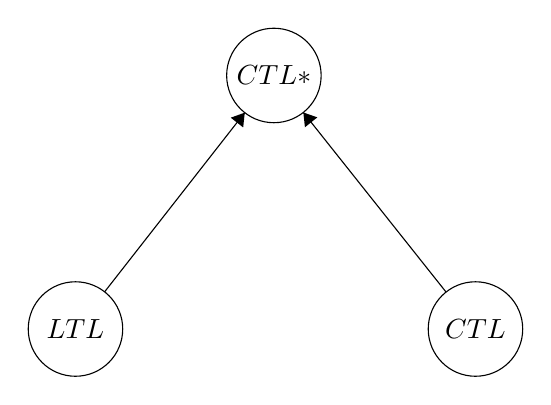
\begin{tikzpicture}[scale=0.2] \tikzstyle{every node}+=[inner sep=0pt] \draw [black] (35.8,-16.1) circle (3); \draw (35.8,-16.1) node {$CTL*$}; \draw [black] (23.2,-32.2) circle (3); \draw (23.2,-32.2) node {$LTL$}; \draw [black] (48.6,-32.2) circle (3); \draw (48.6,-32.2) node {$CTL$}; \draw [black] (25.05,-29.84) -- (33.95,-18.46); \fill [black] (33.95,-18.46) -- (33.06,-18.78) -- (33.85,-19.4); \draw [black] (46.73,-29.85) -- (37.67,-18.45); \fill [black] (37.67,-18.45) -- (37.77,-19.39) -- (38.56,-18.76); \end{tikzpicture} \end{center}

La semantica di queste logiche è basata sulle strutture di Kripke,
ossia 

$\mu=(S,\, I,\,\tau\subseteq S\times S,\, L:\, S\longrightarrow2^{\phi},\, F)$

dove:
\begin{itemize}
\item S è l'insieme degli stati
\item $I\subseteq S$ è l'insieme degli stati iniziali
\item $\tau$ è una relazione tra gli stati totale a sinistra, ossia: $\forall s\in S\,\exists s'\in S\,:\,(s,\, s')\in\tau$
che significa che esistono sempre percorsi di lunghezza infinita.
\item L è la funzione di labelling, che associa ad ogni stato un insieme
di lettere proposizionali, quelle vere nello stato
\item F è l'insieme di stati finali, ovvero l'insieme di stati per cui una
sequenza accettata passa infinitamente spesso
\end{itemize}

\subsection{Grammatica di LTL}

La sintassi di LTL è la più semplice:

una formula ben formata è generata dalla seguente grammatica:

$\varphi\rightarrow P|\neg\varphi|\varphi\wedge\varphi|\varphi\vee\varphi|\varphi\implies\varphi|\varphi\iff\varphi|\next{\varphi}|\eventually{\varphi}|\globally{\varphi}|\until{\varphi}{\varphi}|\release{\varphi}{\varphi}$


\subsection{Grammatica di CTL}

la grammatica di CTL è più complessa, e contiene anche i quantificatori
di cammino, che sono degli operatori che esprimono la verità di una
formula su almeno uno o tutti i cammini, e sono l'operatore E e A
rispettivamente.

i quantificatori di cammino sono vincolati a delle sottoformule specifiche
e non possono essere usati liberamente.

una formula ben formata è generata dalla seguente grammatica:

$\varphi\rightarrow P|\neg\varphi|\varphi\wedge\varphi|\varphi\vee\varphi|\varphi\implies\varphi|\varphi\iff\varphi$

$\varphi\rightarrow A\next{\varphi}|E\next{\varphi}|A\eventually{\varphi}|E\eventually{\varphi}|A\globally{\varphi}|E\globally{\varphi}|A(\until{\varphi}{\varphi})|E(\until{\varphi}{\varphi})|A(\release{\varphi}{\varphi})|E(\release{\varphi}{\varphi})$


\subsection{Grammatica di CTL{*}}

La logica CTL{*} è la logica più complessa e espressiva delle tre.
La sua grammatica è quindi molto più complessa, e si descrive separando
le formule di stato da quelle di cammino:

Sono formule di stato:

$\phi\rightarrow P|\neg\phi|\phi\wedge\phi|\phi\vee\phi|\phi\implies\phi|\phi\iff\phi|A\phi|E\phi$

Sono formule di cammino:

$\varphi\rightarrow\phi|\neg\varphi|\varphi\wedge\varphi|\varphi\vee\varphi|\varphi\implies\varphi|\varphi\iff\varphi|\next{\varphi}|\eventually{\varphi}|\globally{\varphi}|\until{\varphi}{\varphi}|\release{\varphi}{\varphi}$

Le formule di cammino sono formule ben formate (e quindi, anche quelle
di stato).


\subsection{Semantica di CTL{*}}

Per descrivere la semantica di CTL{*} fissiamo una notazione:

sia $\pi$ un cammino $\pi=s_{0},\, s_{1},\, s_{2},\,...$

mentre sia $\pi^{i}$ il suffisso $s_{i},\, s_{i+1},\,...$

$\pi\in s^{\omega}$, ossia appartiene all'insieme delle stringhe
infinite. Si ricordi che:

$s^{\infty}=s^{*}\cup\, s^{\omega}$

La semantica delle formule di stato è definita come:

$\vera{\mu,\pi^{i}}P\iff P\in L(s_{i})$

$\vera{\mu,\pi^{i}}{\neg\phi}\iff\nonvera{\mu,\,\pi^{i}}{\phi}$

$\vera{\mu,\pi^{i}}{\phi\wedge\psi}\iff\vera{\mu,\pi^{i}}{\phi}\,\wedge\,\vera{\mu,\pi^{i}}{\psi}$

$\vera{\mu,\pi^{i}}{\phi\vee\psi}\iff\vera{\mu,\pi^{i}}{\phi}\,\vee\,\vera{\mu,\pi^{i}}{\psi}$

$\vera{\mu,\pi^{i}}{\phi\implies\psi}\iff\nonvera{\mu,\,\pi^{i}}{\phi}\,\vee\,\vera{\mu,\pi^{i}}{\psi}$

$\vera{\mu,\pi^{i}}{(\phi\iff\psi)}\iff(\vera{\mu,\pi^{i}}{\phi}\,\vee\,\vera{\mu,\pi^{i}}{\psi})\vee(\nonvera{\mu,\,\pi^{i}}{\phi}\wedge\nonvera{\mu,\,\pi^{i}}{\psi})$

$\vera{\mu,\pi^{i}}{A\phi}\iff\forall\overline{\pi}\,((\overline{\pi}=s_{i},\,...)\implies(\vera{\mu,\,\overline{\pi}}{\phi))}$

$\vera{\mu,\pi^{i}}{A\phi}\iff\exists\overline{\pi}\,((\overline{\pi}=s_{i},\,...)\implies(\vera{\mu,\,\overline{\pi}}{\phi))}$

La semantica delle formule di cammino è la seguente:

$\vera{\mu,\pi^{i}}{\next{\varphi}}\iff\vera{\mu,\pi^{i+1}}{\varphi}$

$\vera{\mu,\pi^{i}}{\eventually{\varphi}}\iff\exists j\geq i\,:\,\vera{\mu,\pi^{j}}{\varphi}$

$\vera{\mu,\pi^{i}}{\globally{\varphi}}\iff\forall j\geq i\,:\,\vera{\mu,\pi^{j}}{\varphi}$

$\vera{\mu,\pi^{i}}{\until{\varphi}{\psi}}\iff\exists j\geq i\,:\,\vera{\mu,\pi^{j}}{\varphi\,\wedge\,\forall k\,:\, i<k<j}\,\vera{\mu,\,\pi^{k}}{\psi}$

$\vera{\mu,\pi^{i}}{\until{\varphi}{\psi}}\iff\exists j\geq i\,:\,\vera{\mu,\pi^{j}}{\varphi\,\wedge\,\forall k\,:\, i<k<j}\,\vera{\mu,\,\pi^{k}}{\psi}$
<\textcompwordmark{}<sbagliati gli ultimi due, controllare>\textcompwordmark{}>


\section{Model Checking}


\subsection{Definizione}

Il model checking si occupa di risolvere il seguente problema: 

Data una formula $\varphi$ e una struttura di Kripke $\mu$, dire
se $\vera{\mu}{\phi}$ per ogni cammino su $\mu$, ossia:

$\vera{\mu,\,\pi^{0}}{A\varphi}$

In caso contrario esibire un cammino $\pi$ tale che $\nonvera{\mu,\,\pi}{\phi}$\\
\\
Solitamente si verificano 3 tipi di proprietà:
\begin{itemize}
\item Safety: ``non succede mai nulla di grave'' ($\globally{\neg\varphi}$)
\item Liveness: ``prima o poi avviene un evento desiderato'' ($\eventually{\varphi}$)
\item Fairness: ``un evento desiderato avviene infinitamente spesso''
($\globally{\eventually{\varphi}}$)
\end{itemize}
Esistono sostanzialmente due tipologie di tecniche di model checking:
\begin{itemize}
\item Simboliche: basate su tableaux, deduzione formale e SMT solver
\item Operazionali: Basate sulla manipolazione di automi a stati finiti
\end{itemize}

\subsection{Model Checking operazionale}

Il model checking operazionale si basa sulla manipolazione di particolari
automi, detti automi di Büchi.

L'algoritmo alla base è il seguente:
\begin{enumerate}
\item Rappresento il modello $\mu$ con un automa di Büchi $A_{\mu}$
\item per verificare la proprietà $\varphi$, traduco la sua negazione in
un automa di Büchi $A_{\neg\varphi}$
\item Costruisco l'automa prodotto che riconosce il linguaggio intersezione
tra $L(A_{\mu})$ e $L(A_{\neg\varphi})$
\item Controllo se $L(A_{\mu}\times\, A_{\neg\varphi})=\emptyset$, in caso
affermativo la proprietà è verificata.
\end{enumerate}

\subsection{Automi di Büchi}

Gli automi di Büchi sono automi a stati finiti nondeterministici,
che riconoscono linguaggi infiniti, e dove gli stati ``finali''
sono stati di ripetizione, ovvero stati che vengono raggiunti infinite
volte durante il riconoscimento della stringa appartenente al linguaggio.

Gli automi di Büchi godono delle seguenti propietà:

Siano A, B automi di Büchi, allora esiste un automa che riconosce:
\begin{itemize}
\item $L(A)\cup L(B)$
\item $L(A)\cap L(B)$
\item $L(A)^{c}$
\item $L(A)L(B)$ se A è un automa a stati finiti classico
\end{itemize}

\subsection{Da formule di LTL ad automi di Büchi}

Esiste un algoritmo per tradurre una formula di LTL in un automa di
Büchi. Lo stesso algoritmo si può estendere, con le dovute accortezze
e prestando attenzione ai sottocasi, alle formule di CTL e CTL{*}.

Sia $\varphi$ la formula e siano $P_{1},\,...,\, P_{n}$ le lettere
predicative di $\varphi$

Si può trovare un automa di Büchi $A_{\varphi}=(S,\, I,\,\tau,\, L,\, F)$
con $L:\, S\longrightarrow2^{\{P_{1},\,...,\, P_{n}\}}$tale che,
se $\pi$ è un path che corrisponde ad una parola $\omega\in L(A_{\varphi})$,
allora $\vera{(S,\,\tau,\, L),\,\pi}{\varphi}$

l'algoritmo è il seguente:
\begin{enumerate}
\item Porto la formula $\varphi$ in forma negata normale
\item elimino i globally ($\mathcal{G}$)
\item Costruisco l'automa locale $A_{L}$
\item altro che non abbiamo fatto
\end{enumerate}

\subsubsection{Forma negata normale }

Portare una formula in forma negata normale, consiste nel rendere
una formula più ``semplice'', cioè in modo che contenga ``pochi''
connettivi e operatori modali diversi, avendo cura di portare le negazioni
davanti alle lettere proposizionali.

Per farlo utilizzo le seguenti regole:

I) Le relazioni tra gli operatori modali 
\begin{itemize}
\item $\neg\globally{a\equiv\eventually{\neg a}}$
\item $\neg\eventually a\equiv\globally{\neg a}$
\item $\neg(\until a{b)}\equiv(\release{\neg a}{\neg b})$
\item $\neg(\release ab)\equiv(\until{\neg a}{\neg b})$
\end{itemize}
II) Le formule di De Morgan
\begin{itemize}
\item $\neg(a\wedge b)\equiv(\neg a)\vee(\neg b)$
\item $\neg(a\vee b)\equiv(\neg a)\wedge(\neg b)$
\end{itemize}
La formula così trovata si dice in forma negata normale.

Si può a questo punto eliminare anche l'operatore globally, ricordando
la seguante relazione:
\begin{itemize}
\item $\globally a\equiv\release{\bot}a$
\end{itemize}

\subsubsection{Costruzione dell'automa locale}

L'automa locale è un automa che riconosce sequenze di esecuzione che
verificano la proprietà $\varphi$

l'algoritmo si articola in due passi:
\begin{enumerate}
\item Chiusura della formila $\varphi$: $cl(\varphi)$

\begin{itemize}
\item $\varphi\in cl(\varphi)$
\item $\psi\in cl(\varphi)\implies\neg\psi\in cl(\varphi)$
\item $\psi\wedge\theta\in cl(\varphi)\implies\psi,\theta\in cl(\varphi)$
\item $\psi\vee\theta\in cl(\varphi)\implies\psi,\theta\in cl(\varphi)$
\item $\next{\psi}\in cl(\varphi)\implies\neg\psi\in cl(\varphi)$
\item $\eventually{\psi}\in cl(\varphi)\implies\neg\psi\in cl(\varphi)$
\item $\until{\psi}{\theta}\in cl(\varphi)\implies\psi,\theta\in cl(\varphi)$
\item $\release{\psi}{\theta}\in cl(\varphi)\implies\psi,\theta\in cl(\varphi)$
\end{itemize}
\item Automa locale $A_{L}=(\Sigma,\, S_{L},\, I_{L},\,\tau_{L},\, F_{L})$

\begin{itemize}
\item $\Sigma=2^{cl(\varphi)}$ ovvero $\Sigma\subseteq\mathcal{P}(cl(\varphi))$
\item $S_{L}$ formato da tutti gli elementi di $\Sigma$ consistenti ovvero
$\psi\in S_{L}\iff\neg\psi\notin S_{L}$
\item $I_{L}=\{s\in S_{L}\,|\,\varphi\in s\}$
\item $F_{L}=S_{L}$ (ossia tutti gli stati sono finali)
\item $\tau_{L}$ tale che: siano $s,s'\in S_{L}$, $a\in\Sigma$ allora
$(s,\, a,\, s')\in\tau_{L}$ se e solo se:

\begin{enumerate}
\item $a=s$
\item $\next{\psi\in s\iff\psi\in s'}$
\item $\eventually{\psi\in s\iff\psi\in s'\,\vee\,\eventually{\psi\in s'}}$
(infatti vale $\eventually{\psi}\equiv\next{\psi}\vee\next{\eventually{\psi}}$)
\item $\until{\psi}{\theta}\in s\iff\theta\in s'\,\vee\,(\psi\in s\,\wedge\,\until{\psi}{\theta\in s')}$
(infatti vale $\until{\psi}{\theta}\equiv\next{\theta\vee(\psi\wedge\next{(\until{\psi}{\theta}}))}$)
\item $\release{\psi}{\theta}\in s\iff\psi\wedge\theta\in s\,\vee\,(\theta\in s\,\wedge\,\release{\psi}{\theta\in s')}$
\end{enumerate}
\end{itemize}
\end{enumerate}
Una volta costruito l'automa in queosto modo, si deve minimizzare.
L'automa minimo è l'automa locale di $\varphi$


\subsubsection*{Esempio}

<\textcompwordmark{}<MANCA>\textcompwordmark{}>

\end{document}
